%------------------------------------------------------------------------------
%------------------  --------------------------------------------
%----- Bewertung Europäischer Optionen mit Hilfe von Binomialbäumen -----------
% -----------------------------------------------------------------------------
% Autor: Lucas Burger
% E-Mail: Lucas.Burger@uni-konstanz.de
% -----------------------------------------------------------------------------

\documentclass[
    12pt, % Schriftgröße
    DIV10,
    ngerman, % für Umlaute, Silbentrennung etc.
    a4paper, % Papierformat
    oneside, % einseitiges Dokument
    titlepage, % es wird eine Titelseite verwendet
    parskip=half, % Abstand zwischen Absätzen (halbe Zeile)
    headings=normal, % Größe der Überschriften verkleinern
    listof=totoc, % Verzeichnisse im Inhaltsverzeichnis aufführen
    bibliography=totoc, % Literaturverzeichnis im Inhaltsverzeichnis aufführen
    index=totoc, % Index im Inhaltsverzeichnis aufführen
    captions=tableheading, % Beschriftung von Tabellen unterhalb ausgeben
    final % Status des Dokuments (final/draft)
]{scrreprt}


% Meta-Informationen -----------------------------------------------
%    Angaben zur Bachelorarbei, wie z.B. Art, Titel, 
%    Autor, Hochschule etc.
% ---------------------------------------------------------------------


\newcommand{\titel}{Bewertung von Europ\"aischen und Amerikanischen Optionen}
\newcommand{\untertitel}{im Binomial- und Black-Scholes-Modell}
\newcommand{\art}{Bachelorarbeit}
\newcommand{\fachgebiet}{Mathematik und Statistik}
\newcommand{\studiengang}{Mathematische Finanz\"okonomie}
\newcommand{\autor}{Lucas Burger}
\newcommand{\matrikelnr}{01/843636}
\newcommand{\betreuer}{Prof. Dr. Johannes Schropp}
\newcommand{\jahr}{2015}
\newcommand{\ort}{Konstanz}
\newcommand{\logo}{Logo_Uni_Konstanz.jpg}
\newcommand{\wasserzeichen}{Wasserzeichen.jpg}

% Anpassung des Seitenlayouts --------------------------------------------------
%   siehe Seitenstil.tex
% ------------------------------------------------------------------------------
\usepackage[
    automark, % Kapitelangaben in Kopfzeile automatisch erstellen
    headsepline, % Trennlinie unter Kopfzeile
    ilines % Trennlinie linksbündig ausrichten
]{scrpage2}

% Anpassung an Landessprache ---------------------------------------------------
\usepackage[ngerman]{babel}

% Umlaute ----------------------------------------------------------------------
%   Umlaute/Sonderzeichen wie äüöß direkt im Quelltext verwenden (CodePage).
%   Erlaubt automatische Trennung von Worten mit Umlauten.
% ------------------------------------------------------------------------------
\usepackage[utf8]{inputenx}
\usepackage[latin1]{inputenc}

\usepackage{listings}
\lstset{
     literate= {Ö}{{\"O}}1 {Ä}{{\"A}}1 {Ü}{{\"U}}1 {ß}{{\ss}}2 {ü}{{\"u}}1
     {ä}{{\"a}}1 {ö}{{\"o}}1
     }


% Schrift ----------------------------------------------------------------------
\usepackage{lmodern} % bessere Fonts
\usepackage{relsize} % Schriftgröße relativ festlegen

% Grafiken ---------------------------------------------------------------------
% Einbinden von JPG-Grafiken ermöglichen
\usepackage[dvips,final]{graphicx}
\usepackage{transparent}
\usepackage{eso-pic}
\usepackage{float}
% hier liegen die Bilder des Dokuments
\graphicspath{{Bilder/}}

% Befehle aus AMSTeX für mathematische Symbole z.B. \boldsymbol \mathbb --------
\usepackage{amsmath,amsfonts,amsthm,amstext,amssymb}
\usepackage{mathtools}
\usepackage{extarrows}
\usepackage{pgfplots}
\usepackage{tikz}
\usetikzlibrary{matrix}
\usepackage{nicefrac}
\usepackage[]{mcode}

% Define styles for bags and leafs
\tikzstyle{bag} = [text width=2em, text centered]
\tikzstyle{end} = []

% für Index-Ausgabe mit \printindex --------------------------------------------
\usepackage{makeidx}

% Einfache Definition der Zeilenabstände und Seitenränder etc. -----------------
\usepackage{setspace}
\usepackage{geometry}

% Literaturverzeichnis ---------------------------------------------------------
\bibliographystyle{alphadin}

% Symbolverzeichnis ------------------------------------------------------------
%   Symbolverzeichnisse bequem erstellen. Beruht auf MakeIndex:
%     makeindex.exe %Name%.nlo -s nomencl.ist -o %Name%.nls
%   erzeugt dann das Verzeichnis. Dieser Befehl kann z.B. im TeXnicCenter
%   als Postprozessor eingetragen werden, damit er nicht ständig manuell
%   ausgeführt werden muss.
%   Die Definitionen sind ausgegliedert in die Datei "Glossar.tex".
% ------------------------------------------------------------------------------
\usepackage[intoc]{nomencl}
\let\abbrev\nomenclature
\renewcommand{\nomname}{Abkürzungsverzeichnis}
\setlength{\nomlabelwidth}{.25\hsize}
\renewcommand{\nomlabel}[1]{#1 \dotfill}
\setlength{\nomitemsep}{-\parsep}

% zum Umfließen von Bildern ----------------------------------------------------
%\usepackage{floatflt}


% zum Einbinden von Programmcode -----------------------------------------------
\usepackage{listings}
\usepackage{xcolor,soul} 
\definecolor{hellgelb}{rgb}{1,1,0.85}
\definecolor{colKeys}{RGB}{0,0,255}
\definecolor{colIdentifier}{rgb}{0,0,0}
\definecolor{colComments}{RGB}{34,139,34}
\definecolor{colString}{RGB}{160,32,240}
\lstset{
    float=hbp,
    basicstyle=\ttfamily\color{black}\small\smaller,
    identifierstyle=\color{colIdentifier},
    keywordstyle=\color{colKeys},
    stringstyle=\color{colString},
    commentstyle=\color{colComments},
    columns=flexible,
    tabsize=2,
    frame=single,
    extendedchars=true,
    showspaces=false,
    showstringspaces=false,
    numbers=left,
    numberstyle=\tiny,
    breaklines=true,
    backgroundcolor=\color{white},
    breakautoindent=true
}

% URL verlinken, lange URLs umbrechen etc. -------------------------------------
\usepackage{url}

% wichtig für korrekte Zitierweise ---------------------------------------------
\usepackage[square]{natbib}

% PDF-Optionen -----------------------------------------------------------------
\usepackage[
    bookmarks,
    bookmarksopen=true,
    colorlinks=true,
% diese Farbdefinitionen zeichnen Links im PDF farblich aus
    linkcolor=red, % einfache interne Verknüpfungen
    anchorcolor=black,% Ankertext
    citecolor=blue, % Verweise auf Literaturverzeichniseinträge im Text
    filecolor=magenta, % Verknüpfungen, die lokale Dateien öffnen
    menucolor=red, % Acrobat-Menüpunkte
    urlcolor=cyan, 
% diese Farbdefinitionen sollten für den Druck verwendet werden (alles schwarz)
    %linkcolor=black, % einfache interne Verknüpfungen
    %anchorcolor=black, % Ankertext
    %citecolor=black, % Verweise auf Literaturverzeichniseinträge im Text
    %filecolor=black, % Verknüpfungen, die lokale Dateien öffnen
    %menucolor=black, % Acrobat-Menüpunkte
    %urlcolor=black, 
    backref,
    plainpages=false, % zur korrekten Erstellung der Bookmarks
    pdfpagelabels, % zur korrekten Erstellung der Bookmarks
    hypertexnames=false, % zur korrekten Erstellung der Bookmarks
    linktocpage % Seitenzahlen anstatt Text im Inhaltsverzeichnis verlinken
]{hyperref}
% Befehle, die Umlaute ausgeben, führen zu Fehlern, wenn sie hyperref als Optionen übergeben werden
\hypersetup{
    pdftitle={\titel \untertitel},
    pdfauthor={\autor},
    pdfcreator={\autor},
    pdfsubject={\titel \untertitel},
    pdfkeywords={\titel \untertitel},
}

% fortlaufendes Durchnummerieren der Fußnoten ----------------------------------
\usepackage{chngcntr}

% für lange Tabellen -----------------------------------------------------------
\usepackage{longtable}
\usepackage{array}
\usepackage{ragged2e}
\usepackage{lscape}

% Spaltendefinition rechtsbündig mit definierter Breite ------------------------
\newcolumntype{w}[1]{>{\raggedleft\hspace{0pt}}p{#1}}

% Formatierung von Listen ändern -----------------------------------------------
\usepackage{paralist}

% bei der Definition eigener Befehle benötigt
\usepackage{ifthen}

% definiert u.a. die Befehle \t'odo und \listoft'odos
\usepackage{todonotes}

% sorgt dafür, dass Leerzeichen hinter parameterlosen Makros nicht als Makroendezeichen interpretiert werden
\usepackage{xspace}

\usepackage{blindtext}


\makeindex


% Seitenstil

% Zeilenabstand 1,5 Zeilen -----------------------------------------------------
\onehalfspacing

% Seitenränder -----------------------------------------------------------------
\setlength{\topskip}{\ht\strutbox} % behebt Warnung von geometry
\geometry{paper=a4paper,left=40mm,right=20mm,top=20mm}

% Kopf- und Fußzeilen ----------------------------------------------------------
\pagestyle{scrheadings}
% Kopf- und Fußzeile auch auf Kapitelanfangsseiten
\renewcommand*{\chapterpagestyle}{scrheadings} 
% Schriftform der Kopfzeile
\renewcommand{\headfont}{\normalfont}

% Kopfzeile
\ihead{\normal{\textsc{\titel}}\\ \small{\untertitel} \\[1mm] \textit{\headmark}}
\chead{}
\ohead{\pagemark}
\setlength{\headheight}{21mm} % Höhe der Kopfzeile
% Kopfzeile über den Text hinaus verbreitern
%\setheadwidth[0pt]{textwithmarginpar} 
\setheadsepline[text]{0.4pt} % Trennlinie unter Kopfzeile

% Fußzeile
\ifoot{\copyright\ \autor}
\cfoot{}
\ofoot{\pagemark}
\addtolength{\footskip}{-1cm} % Fußzeile 1 cm höher setzen

% sonstige typographische Einstellungen ----------------------------------------

% erzeugt ein wenig mehr Platz hinter einem Punkt
\frenchspacing 

% Schusterjungen und Hurenkinder vermeiden
\clubpenalty = 10000
\widowpenalty = 10000 
\displaywidowpenalty = 10000

% Quellcode-Ausgabe formatieren
\lstset{numbers=left, numberstyle=\tiny, numbersep=5pt, breaklines=true}
\lstset{emph={square}, emphstyle=\color{red}, emph={[2]root,base}, emphstyle={[2]\color{blue}}}

% Fußnoten fortlaufend durchnummerieren
\counterwithout{footnote}{chapter}



% Befehle

% Eigene Befehle und typographische Auszeichnungen für diese

% einfaches Wechseln der Schrift, z.B.: \changefont{cmss}{sbc}{n}
\newcommand{\changefont}[3]{\fontfamily{#1} \fontseries{#2} \fontshape{#3} \selectfont}

% Abkürzungen mit korrektem Leerraum 
\newcommand{\ua}{\mbox{u.\,a.\ }}
\newcommand{\zB}{\mbox{z.\,B.\ }}
\newcommand{\dahe}{\mbox{d.\,h.\ }}
\newcommand{\Vgl}{Vgl.\ }
\newcommand{\bzw}{bzw.\ }
\newcommand{\evtl}{evtl.\ }

\newcommand{\abbildung}[1]{Abbildung~\ref{fig:#1}}

\newcommand{\bs}{$\backslash$}

% erzeugt ein Listenelement mit fetter Überschrift 
\newcommand{\itemd}[2]{\item{\textbf{#1}}\\{#2}}

% einige Befehle zum Zitieren --------------------------------------------------
\newcommand{\Zitat}[2][\empty]{\ifthenelse{\equal{#1}{\empty}}{\citep{#2}}{\citep[#1]{#2}}}

% zum Ausgeben von Autoren
\newcommand{\AutorName}[1]{\textsc{#1}}
\newcommand{\Autor}[1]{\AutorName{\citeauthor{#1}}}

% verschiedene Befehle um Wörter semantisch auszuzeichnen ----------------------
\newcommand{\NeuerBegriff}[1]{\textbf{#1}}
\newcommand{\Fachbegriff}[1]{\textit{#1}}

\newcommand{\Eingabe}[1]{\texttt{#1}}
\newcommand{\Code}[1]{\texttt{#1}}
\newcommand{\Datei}[1]{\texttt{#1}}

\newcommand{\Datentyp}[1]{\textsf{#1}}
\newcommand{\XMLElement}[1]{\textsf{#1}}
\newcommand{\Webservice}[1]{\textsf{#1}}


\begin{document}
\pagenumbering{roman}
% Deckblatt

\thispagestyle{plain}
\begin{titlepage}

\begin{center}

\huge{\textbf{\titel}}\\[1.5ex]
\LARGE{\textbf{\untertitel}}\\[8ex]
\Large{\textbf{\art} zur Erlangung des \\ Grades Bachelor of Science}\\[1.5ex]
\Large{im Fachbereich \fachgebiet \\ der Universit\"at Konstanz}\\[10ex]


\normalsize
\hspace{20mm}
\begin{tabular}{rl} \\

vorgelegt von:        & \quad \autor                 \\
                      & \quad Mosbruggerstr. 17      \\
                      & \quad 78462 Konstanz         \\[1.2ex]  
Studienfach:          & \quad \studiengang           \\[1.2ex]
Bearbeitungszeitraum: & \quad 11.11.15 bis 11.01.16  \\[1.2ex]
Gutachter:            & \quad \betreuer              \\[1.2ex]
\end{tabular}

\copyright\ \jahr \\
\end{center}

\AddToShipoutPicture*{
    \put(0,-65){
        \parbox[b][\paperheight]{\paperwidth}{
            \vfill
            \centering
            {\transparent{0.2}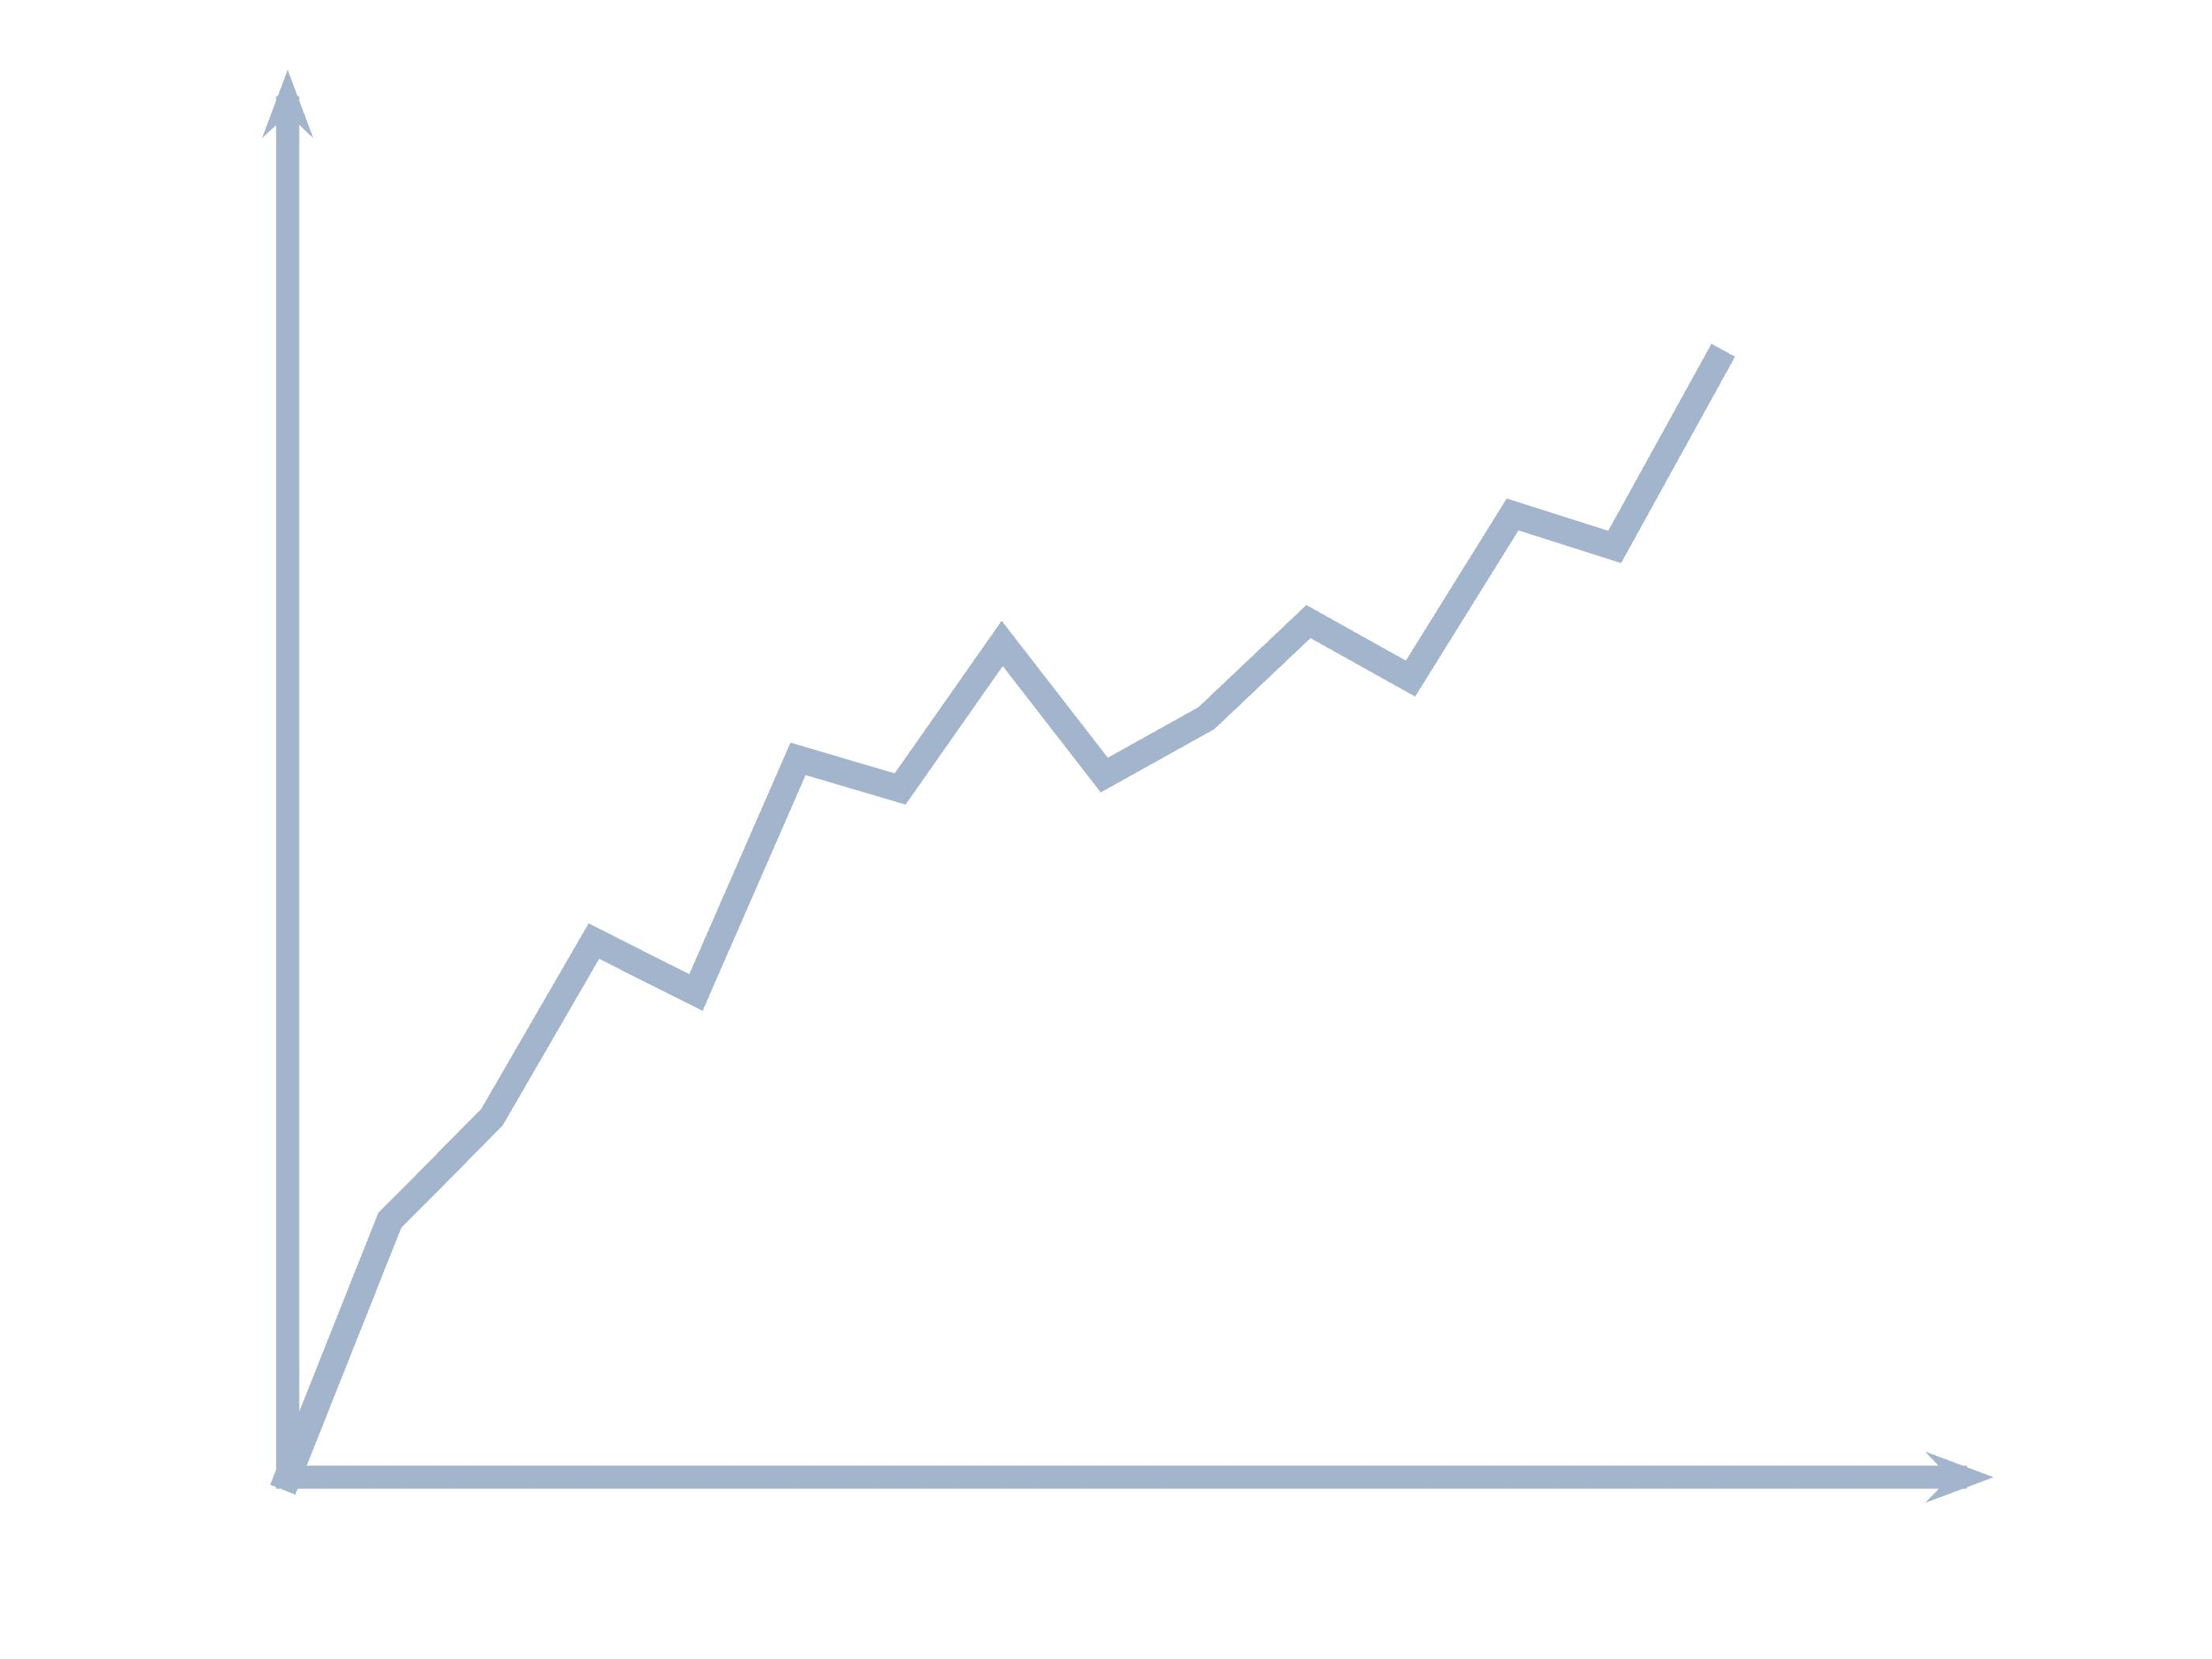
\includegraphics[width=1.47\textwidth]{BBW.jpg}}%
            \vfill
        }
    }
}

\smallbreak
%\noindent Dieses Werk ist \textbf{urheberrechtlich gesch\"utzt}. Eine Verwendung oder Vervielf\"altigung ohne die Zustimmung des Autors ist strafbar.

\end{titlepage}

\tableofcontents


% Zusammenfassung

\pagenumbering{arabic}
\chapter{Einleitung}


Am modernen Finanzmarkt gewinnen Derivate immer mehr an Bedeutung und Handelsvolumen. Derivate sind Finanzinstrumente, deren Wert über den Wert und die Preisentwicklung eines anderen handelbaren Gutes bestimmt werden (lat. \textit{derivare} = \glqq ableiten\grqq). Gezielt gewählte Derivate bilden damit eine gute Möglichkeit, sich gegen Schocks oder ungünstige Kursentwicklungen des zugrundeliegenden Gutes abzusichern und gewinnen so ihre Beliebtheit.
Im Rahmen dieser Arbeit wollen wir uns Optionen anschauen. Optionen können auf verschiedene Güter (sogenannte Basiswerte) und zu vielen verschiedenen Konditionen geschrieben sein. Wir werden \glqq Europäische und Amerikanische Call- und Put-Optionen\grqq\,, deren Basiswert eine Aktie ist, anschauen und Modelle und Methoden herleiten, um den Preis -- den Betrag, der bei Vertragsschluss ausgetauscht wird -- dieser Derivate zu bestimmen. Natürlich bestimmt sich der tatsächliche Preis dieser Optionen nicht nach mathematischen Formeln und Gleichungen, sondern über Angebot und Nachfrage am Markt. Dennoch bilden die in dieser Arbeit vorgestellten Modelle (das Binomial- und das Black-Scholes-Modell) stets eine Orientierung für alle Markteilnehmer.

\vspace{0.8cm}
{\large\bf{Zusammenfassung}}

Zunächst wird im 2. Kapitel auf den wirtschaftlichen Hintergrund und die mathematischen Grundlagen eingegangen, welche für die Arbeit von zentraler Bedeutung sind. Anschließend werden wir in Kapitel 3 das zeitdiskrete Binomialmodell herleiten und auf dessen Konvergenz eingehen, um anschließend unsere Überlegungen teils auf das 4. Kapitel zu übertragen. In diesem werden wir auf das kontinuierliche Black-Scholes-Modell übergehen werden und dort zunächst, sofern möglich, einen analytischen Ansatz zur Optionsbewertung wählen. Da es allerdings für die Amerikanschen Optionen keinen analytischen Ansatz gibt, werden wir diese mithilfe numerischer Methoden (angelehnt an \cite{GuentherJuengel}) approximieren, wodurch wir auch Algorithmen für die Europäischen Optionen erhalten werden. Zuletzt werden wir uns in Kapitel 5 die hergeleiteten Algorithmen und deren Korrektheit an kurzen Beispielen anschauen, deren Implementierung im Anhang zu finden sind.

% Ökonomische und mathematische Grundlagen zur Bewertung von Optionen

\chapter{Grundlagen}


Um in das Thema der Optionsbewertung einsteigen zu können, bedarf es einiger Grundlagen, die im Folgenden geschaffen werden. Dabei geht es zum Einen um stochastische Prozesse und Itô's Lemma, zum Anderen um einige Begriffsklärungen, die für das Verständnis des ökonomischen Hintergrundes wichtig sind (z.B. Aktie, Option, Arbitrage...). Für tiefergehende Literatur sei auf \cite{Hull} (Ökonomisch) und \cite{Kupper1}/\cite{Kupper2} bzw. \cite{Bauer} (Mathematisch) verwiesen.

\newtheoremstyle{normal}% normale Schrift
{10pt}% hSpace abovei
{10pt}% hSpace belowi
{\normalfont}% hBody fonti
{}% hIndent amounti1
{\normalfont}% hTheorem head fonti
{}% Punctuation after theorem headi
{0.8em}% hSpace after theorem headi2
{\bfseries{\thmname{#1}\thmnumber{ #2}.\thmnote{ \hspace{0.2em}(#3)}}}% hTheorem head spec (can be left empty, meaning `normal')
 


\theoremstyle{normal}
\newtheorem{Definition}{Definition}[chapter]
\newtheorem{satz}[Definition]{Satz}
\newtheorem{bsp}[Definition]{Beispiel}
\newtheorem{Lemma}[Definition]{Lemma}
\newtheorem{Theorem}[Definition]{Theorem} 
\newtheorem*{Bemerkung}{Bemerkung}



%%%%%%%%%%%%%%%%%%%%%%%%%%%%%%%%%%%%%%%%%%%%%%%%%%%%%%%%%%%%%%%%%%%%%%%%%%%%%%
\section{Mathematische Grundlagen}            %%%%%%%%%%%%%%%%%%%%%%%%%%%%%%%%
\label{cha:MathematischeGrundlagen}           %%%%%%%%%%%%%%%%%%%%%%%%%%%%%%%%
%%%%%%%%%%%%%%%%%%%%%%%%%%%%%%%%%%%%%%%%%%%%%%%%%%%%%%%%%%%%%%%%%%%%%%%%%%%%%%

Sei $ \left(\Omega,\mathcal{F},\mathbb{P}\right) $ ein Wahrscheinlichkeitsraum über einem Ereignisraum $\Omega$, sowie einer $\sigma\text{-Algebra  }\mathcal{F}$ und einem Wahrscheinlichkeitsmaß $\mathbb{P}$.
%%%%%%%%%%%%%%%%% Stochastischer Prozess %%%%%%%%%%%%%%%%%%%%%%%%%%
\begin{Definition}
Ein (stetiger) stochastischer Prozess $\left(X_t\right)_{t\geq0}$ auf einem Wahrscheinlichkeitsraum $ \left(\Omega,\mathcal{F},\mathbb{P}\right) $ ist eine Folge von Zufallsvariablen  $X: \Omega \times \left[0,\infty \right) \mapsto \mathbb{R} $. Für ein festes $\omega \in \Omega$ ergibt sich ein stetiger Pfad $t \mapsto X\left(\omega,t\right)$.
\end{Definition}

%%%%%%%%% Brownsche Bewegung %%%%%%%%%%%%%%%%%%%%%
\begin{Definition}[Brown'sche Bewegung]
Ein stochastischer Prozess $\left(W_t\right)_{t\geq0}$ mit den Eigenschaften
\begin{enumerate}
\item $W_0 = 0 \,\,\mathbb{P}\textit{-fast sicher, d.h. } \mathbb{P}\left(\omega \in \Omega : W\left(0,\omega\right) \neq 0 \right) = 0 $.
\item $\textit{Die Inkremente } W_t - W_s \textit{ für } t>s \textit{ sind } \mathcal{N}(0,t-s) \textit{-verteilt}$.
\item $\textit{Für alle } 0\leq t_1 < t_2 < ... < t_n \textit{ sind } W_{t_2} - W_{t_1}, \, ... \, ,W_{t_n}-W_{t_{n-1}} \\ \textit{unabhängig}$.
\end{enumerate}
wird Brown'sche Bewegung oder Wiener Prozess genannt.
\end{Definition}

%%%%%%%%%%% Itô-Prozess %%%%%%%%%%%%%%%%%%%%%%%%%%%%
\begin{Definition} \label{def:ito-Prozess}
Sei $\left(X_t\right)_{t\geq0}$ ein stochastischer Prozess. Eine stochastische Differentialgleichung nach Itô ist von der Form
\begin{equation}
dX_t = a(X_t,t)dt + b(X_t,t)dW_t \label{def:ito-DGL}
\end{equation}
mit hinreichend regulären Funktionen $a(x,t)$ und $b(x,t)$ und ist äquivalent zu folgender Integralgleichung:
\begin{equation}
X_t = X_0 + \int_0^t \! a(X_s,s) ds + \int_0^t \! b(X_s,s)dW_s
\end{equation}
Hierbei ist das erste ein gewöhnliches Lebesgue-Integral und das zweite ein sogenanntes Itô-Integral über eine Brown'sche Bewegung $\left(W_t\right)_{t\geq0}$.
\end{Definition}

Ein (stochastischer) Prozess $X_t$  wird Itô-Prozess genannt, wenn er von obiger Form ist. In diesem werden $a(X_t,t)dt$ als  \glqq Drift-Term\grqq \, und $b(X_t,t)dW_t$ als \glqq Diffusions-Term\grqq \,bezeichnet.


%%%%%%%%%%%%%%% Itô's Lemma %%%%%%%%%%%%%%%%%%
\begin{Lemma}[Itô]\label{GL:itosLemma}
Sei $f \in C^{2,1}(\mathbb{R}, \mathbb{R}^+), \, T \in \mathbb{R}^+ \textit{ und } X = \left(X_t\right)_{t\geq0}$ ein Itô-Prozess. Dann ist $f(X_t,t)$ ein Itô-Prozess und es gilt für jedes $t \in \left[0,T\right]$:
\begin{eqnarray*}
f(X_t,t) & = & f(0,0) + \int_0^t \! \left( \frac{\partial f}{\partial t} \left(X_s,s\right) + a\frac{\partial f}{\partial x}\left(X_s,s\right) + b^2 \frac{1}{2} \frac{\partial ^2 f}{\partial x^2}\left(X_s,s\right) \right) ds \\
 & & + \int_0^t \! b\frac{\partial f}{\partial x}\left(X_s,s\right) \, dW 
\end{eqnarray*}
beziehungsweise als Differentialgleichung (unter Fortlassung der Argumente):
\begin{equation}
df = \left( \frac{\partial f}{\partial t}  + a\frac{\partial f}{\partial x} + b^2 \frac{1}{2} \frac{\partial ^2 f}{\partial x^2} \right)dt + b\frac{\partial f}{\partial x}dW_s
\end{equation}

\begin{proof}
Für den Beweis dieses Lemmas wird auf \cite{Kupper2} verwiesen.
\end{proof}

\end{Lemma}

\begin{Bemerkung}
In weiteren Verlauf werden partielle Ableitungen von Funktionen mit einem Subskirpt geschrieben, also $ \frac{\partial f}{\partial t} = f_t $ oder $\frac{\partial ^2 f}{\partial x^2} = f_{xx}$.
\end{Bemerkung}



%%%%%%%%%%%%%%%%%%%%%%%%%%%%%%%%%%%%%%%%%%%%%%%%%%%%%%%%%%%%%%%%%%%%
\section{Ökonomische Grundlagen}        %%%%%%%%%%%%%%%%%%%%%%%%%%%%
%%%%%%%%%%%%%%%%%%%%%%%%%%%%%%%%%%%%%%%%%%%%%%%%%%%%%%%%%%%%%%%%%%%%
In diesem Abschnitt werden einige wichtige Begriffe erläutert und grundlegende Annahmen getroffen.

\begin{Definition}[Aktie]
Eine Aktie ist ein verbriefter Anteilsschein an einem Unternehmen. Dieser kann an der Börse zu aktuellen Kursen ge- und verkauft werden. Diese Unternehmen - sogenannte Aktiengesellschaften (AG) - nutzen den Verkauf von Aktien zur Beschaffung von Eigenkapital.
\end{Definition}

\begin{Definition}[Dividende]
Eine Dividende ist ein Gewinnanteil eines Unternehmens, der an die Aktionäre (die Besitzer der Aktien) ausgeschüttet wird.
\end{Definition}


\begin{Definition}[Option]
Eine Option ist ein zwischen zwei Parteien abgeschlossener Vertrag, der dem Käufer das Recht, nicht die Pflicht, einräumt, eine Aktie (S) zu einem im Vorraus festgelegten Preis (K, genannt \glqq Strike Price\grqq) zu kaufen (Call-Option) oder zu verkaufen (Put-Option). Man sagt dann, \glqq er übt seine Option aus\grqq. Bei einer \textit{Europäischen Option} darf er dies nur zu \textit{einem bestimmten} Zeitpunkt in der Zukunft tun, bei einer \textit{Amerikanischen Option} darf er auch \textit{zu jedem früheren} Zeitpunkt ausüben. Das Ende dieser Laufzeit wird mit $T$ beschrieben und Fälligkeit genannt.
\end{Definition}

Optionen bringen je nach Typ und Kursentwicklung des zugrundeliegenden Wertpapieres einen Gewinn ein. Besitzt man eine Call-Option zum Strike Price $K$ und die zugrundeliegende Aktie habe zum Zeitpunkt $T$ den Wert $S_T$, so kann man durch Ausüben der Option einen Gewinn realisieren, wenn $S_T>K$. Falls $S_T \leq K$, kann man keinen Gewinn erzielen und die Option wird nicht ausgeübt.
Allgemein kann der Wert $V(S_T,T)$ einer Call-Option mit Strike Price $K$ zum Fälligkeitsdatum $T$ also geschrieben werden als (siehe Anhang \ref{Anhang:PlotPayoff}):

\begin{equation*}
V^C\left(S,T\right) = 
\begin{cases}
S_T - K   & \text{ falls }     S_T > K           \textit{   (Option wird ausgeübt)} \\
0         & \text{ falls }     S_T \leq K      \textit{   (Option verfällt)}  
\end{cases}
\end{equation*}
oder kompakter
\begin{equation}
V^C\left(S,T\right) = \left(S_T-K\right)^+ \coloneqq max\left\{S_T-K,0\right\} \label{GL:payoffCall}
\end{equation}
Analog ergibt sich für den Wert einer Put-Option:
\begin{equation}
V^P\left(S,T\right) = \left(K-S_T\right)^+ \coloneqq max\left\{K-S_T,0\right\} \label{GL:payoffPut}
\end{equation}

Für die Auszahlungsfunktion\footnote{Da die Option nur das Kaufrecht darstellt, hat sie selbst keine Auszahlung. Gemeint ist der Erlös durch Ausüben der Option und sofortiges (ver-)kaufen der erworbenen/verkauften Aktie.} werden wir $\Lambda (S) = \left(S-K\right)^+$ für die Call-Option und $\Lambda (S) = \left(K-S\right)^+$ für die Put-Option schreiben.


\begin{Definition}[Arbitrage]
Arbitrage ist die Möglichkeit ohne Kapitaleinsatz einen sofortigen Gewinn zu realisieren. Arbitrage kann durch eine ungleiche Bepreisung eines Gutes in verschiedenen Märkten entstehen. Damit kann ein Arbitrageur dieses Gut zu einem günstigeren Preis kaufen und zum gleichen Zeitpunkt (woanders) zu einem teureren verkaufen und erzielt damit einen sofortigen, risikolosen Gewinn.
\end{Definition}


Um eine korrekte Bepreisung der Optionen zu garantieren, diese aber auch gleichzeitig einfach zu halten, werden verschiedene Annahmen gemacht:
\begin{enumerate}
\item Der Finanzmarkt ist friktionslos, d.h. es werden weder Transaktionskosten, noch Steuern für Käufe oder Verkäufe erhoben.
\item Leerverkäufe sind erlaubt, was bedeutet, dass man etwas verkaufen kann, obwohl man es noch gar nicht besitzt.
\item Es kann stetig gehandelt werden und Anlagen sind beliebig teilbar. Es können also Bruchteile von z.B. einer Aktie verkauft werden. Ebenso werden Anlagen stetig  verzinst und Dividenden stetig ausbezahlt.
\end{enumerate}






\chapter{Binomialmodell}
\label{cha:binomialmodell}

In diesem Kapitel werden wir den Verlauf der zugrundeliegenden Aktie modellieren. Dabei werden wir uns das Prinzip des Binomialbaums zunächst für eine einzelne Periode $\Delta t$ anschauen. Danach werden wir dieses Konzept auf mehrere Perioden übertragen, um eine bessere Darstellung unseres Aktienkurses $S_t$ (das ist der Wert der Aktie zum Zeitpunkt t) zu erhalten. Wir werden anschließend eine Formel herleiten und damit den Wert der Option bestimmen. Als letztes werden wir uns anschauen, ob und gegen welchen Wert der Optionspreis für immer kleinere Schrittweiten $\Delta t$ konvergiert.

%%%%%%%%%%%%%%%%%%%%%%%%%%%%%%%%%%%%%%%%%%%%%%%%%%%%%%%%%%%%%%%%%%%
\section{Ein-Perioden-Modell}        %%%%%%%%%%%%%%%%%%%%%%%%%%%%%%
\label{cha:Ein-Perioden-Modell}      %%%%%%%%%%%%%%%%%%%%%%%%%%%%%%
%%%%%%%%%%%%%%%%%%%%%%%%%%%%%%%%%%%%%%%%%%%%%%%%%%%%%%%%%%%%%%%%%%%
Im Binomialmodell wird angenommen, dass die Kursentwicklung einer Aktie sich gemäß einer binomialverteilten Zufallsvariable verhält. In jedem Zeitschritt kann die Aktie mit einer Wahrscheinlichkeit $q$ um den Faktor $u > 1$ steigen, oder mit der Wahrscheinlichkeit $1-q$ um den Faktor $d < 1$ fallen.
Für eine einzelne Periode $\Delta t$ ergibt sich folgende Kursentwicklung:

\begin{figure}[htbp!]
    \begin{tikzpicture}[sloped]
        \node (z) at (-3,0) [bag] {};
        % Aktie
  	    \node (a) at (0,0) [bag] {$S_0$};
 	    \node (b) at (3,-1) [bag] {$S^u(\Delta t)$};
  	    \node (c) at (3,1) [bag] {$S^d(\Delta t)$};
  	    % Zeichnen der Pfeile
	    \draw [->] (a) to node [below] {$1-q$} (b);
  	    \draw [->] (a) to node [above] {$q$} (c);
	    % Anleihe
	    % Anlegen der Knoten
  	    \node (d) at (5.5,0) [bag] {$B(0)$};
 	    \node (e) at (8,0) [bag] {$B(\Delta t)$};
  	    % Zeichnen des Pfeils	
	    \draw [->] (d) to node [below] {} (e);  
    \end{tikzpicture}
    \caption{Entwicklung der Aktie und der Anleihe im Intervall $\left[0,\Delta t\right]$}
\end{figure}

Zudem nehmen wir an, dass unser Finanzmarkt neben der Aktie nur aus einem risikolosen Anleihe $B(t)$ (engl. Bond), welcher mit Zinssatz $r$ stetig verzinst wird, und einer zu bewertenden Call-Option besteht. Wir wollen uns nun ein Portfolio aus $c_1$ Anteilen der Anleihe und $c_2$ Anteilen der Aktie konstruieren, sodass zu jedem Zeitpunkt $ t \in \left\{0,\Delta t\right\} $ und jedem Zustand gilt:
\begin{equation*}
c_1 \cdot B(t) + c_2 \cdot S_t \, = \,C(t) \, = \left(S_t - K \right) ^+ 
\end{equation*}
Nachdem sowohl die Aktie, als demnach auch die Option zum Zeitpunkt $\Delta t$ zwei Zustände annehmen kann, erhalten wir folgendes Gleichungssystem:
\begin{eqnarray*}
c_1 \cdot B^u(\Delta t) + c_2 \cdot S^u(\Delta t) & = & C_u(\Delta t) \\
c_1 \cdot B^d(\Delta t) + c_2 \cdot S^d(\Delta t) & = & C_d(\Delta t)
\end{eqnarray*}
Ohne Beschränkung der Allgemeinheit kann $B(0) = 1$ gesetzt werden. Da die Anleihe risikolos ist, gilt $B^u(\Delta t) = B^d(\Delta t) = e^{r\Delta t}$ und wir erhalten durch Einsetzen von $S^u(\Delta t)$ und $S^d(\Delta t)$:
\begin{eqnarray}
c_1 \cdot e^{r\Delta t} + c_2 \cdot uS & = & C_u(\Delta t) \nonumber \label{Bin:gleichungssystem} \\
c_1 \cdot e^{r\Delta t} + c_2 \cdot dS & = & C_d(\Delta t)  
\end{eqnarray}
Und die Lösung dieses Gleichungssystems lautet (siehe Anhang \ref{Anhang:LGS}):
\[
		c_1 = \frac{uC_d - dC_u}{(u - d)e^{r\Delta t}} \quad , \quad c_2 = \frac{C_u - C_d}{(u-d)S}  
\]
Da $c_1$ und $c_2$ nun so gewählt sind, dass das Portolio genau die Call-Option repliziert, ergibt sich ihr Preis als der Wert des Portfolios zum Zeitpunkt $t=0$ und mit $S_0 = S$ folgt:
\begin{eqnarray}    
C_0  = c_1 \cdot 1 + c_2 \cdot S    & = & \frac{uC_d - dC_u}{(u - d)e^{r\Delta t}} \cdot 1 + \frac{C_u - C_d}{(u-d)S} \cdot S \nonumber \\
                                    & = & \frac{uC_d - dC_u}{(u - d)e^{r\Delta t}} \cdot 1 + \frac{C_ue^{r\Delta t} - C_de^{r\Delta t}}{(u-d)e^{r\Delta t}} \nonumber \\ 
                                    & = & e^{-r\Delta t} \left( \frac{e^{r\Delta t} - d}{u-d} \cdot C_u + \frac{u - e^{r\Delta t}}{u-d}\cdot C_d\right) \nonumber \\
                                    & = & e^{-r\Delta t}\left(pC_u + (1-p)C_d\right) \nonumber \\ 
		  	 	 				  & = & e^{-r\Delta t} \mathbb{E}_p\left[C_{\Delta t}\right] \label{BIN:1PeriodenCall}
\end{eqnarray}
Mit $ 0 \leq p = \frac{e^{r\Delta t} - d}{u-d} \leq 1 $ als die sogenannte \glqq risikoneutrale Wahrscheinlichkeit\grqq\, und $\mathbb{E}_p\left[ \,\cdot\, \right]$ als der Erwartungswert unter $p$. Durch Multiplikation mit dem Diskontfaktor $e^{-r\Delta t}$ erhalten wir den Barwert - respektive den Preis - unserer Option.

Dass der Preis der Option genau dem des Portfolios entspricht, folgt aus der Annahme der Arbitragefreiheit. Da beide das gleiche Gut liefern, könnte man bei einem Preisunterschied durch den Einkauf des günstigeren und gleichzeitigem Verkauf des teureren einen risikolosen Gewinn erzielen.

Das bedeutet, dass wir zu einer Aktie $S$ mit gegebenen Parametern $u, \, d \text{ und } q$ den Wert einer Call-Option bestimmen können. Da unser Modell mit nur einer Periode allerdings sehr einschränkend ist, wollen wir unsere Überlegungen im Folgenden auf $n \geq 2$ Perioden übertragen.

%%%%%%%%%%%%%%%%%%%%%%%%%%%%%%%%%%%%%%%%%%%%%%%%%%%%%%%%%%%%%%%%%
\section{n-Perioden-Modell}                 %%%%%%%%%%%%%%%%%%%%%
%%%%%%%%%%%%%%%%%%%%%%%%%%%%%%%%%%%%%%%%%%%%%%%%%%%%%%%%%%%%%%%%%

Mit der Erweiterung auf mehrere Perioden erhalten wir durch die breitere Streuung und den detaillierteren Verlauf des Kurses eine bessere Modellierung unseres Options- bzw. Aktienkurses. Wir betrachten einen Zeithorizont $T$, der in n Zeitschritte der Länge $\Delta t = \frac{T}{n}$ unterteilt wird. Mit $S_k^n \coloneqq u^kd^{n-k}S$ erhalten einen n-Perioden Binomialbaum für die Entwicklung des Aktienkurses:
\begin{figure}[htbp!] \label{BIN:BinomialbaumAktie}
\begin{tikzpicture}[sloped]
		\node (z) at (-2,0) [bag] {};
		% Anlegen der Knoten
		% 1
  			\node (a) at (0,0) [bag] {$S_0$};
		% 2
 		 	\node (b) at (2.5,-0.5) [bag] {$S_0^1$};
  			\node (c) at (2.5,0.5) [bag] {$S_1^1$};
		% 3
  			\node (d) at (5,-1) [bag] {$S_0^2$};
  			\node (e) at (5,0) [bag] {$S_1^2$};
  			\node (f) at (5,1) [bag] {$S_2^2$};
		% 4
			\tikzstyle{bag} = [text width=0.5em, text centered]
  			\node (g) at (6.5,-1) [bag] {};
  			\node (h) at (6.5,0) [bag] {};
  			\node (i) at (6.5,1) [bag] {};
  			\tikzstyle{bag} = [text width=0.5em, text centered]
		% 5
  			\node (j) at (9,-1.5) [bag] {$S^n_0$}; % Cuuuuuuuuu
  			\node (k) at (9,-0.5) [bag] {$S^n_1$};
 			\node (l) at (9, 0.5) [bag] {$S_{n-1}^n$};
  			\node (m) at (9,1.5)[bag] {$S_n^n$};
  		% Zeichnen der Pfeile
		% 1
			\draw [->] (a) to node [below] {$1-q$} (b);
  			\draw [->] (a) to node [above] {$q$} (c);
  		%2
  			\draw [->] (c) to node [above] {} (f);
  			\draw [->] (c) to node [above] {} (e);
  			\draw [->] (b) to node [above] {} (e);
  			\draw [->] (b) to node [below] {} (d);
  		%3
  			\draw [line width=1.1pt, style=loosely dotted] (d) to node [above] {} (g);
  			\draw [line width=1.1pt, style=loosely dotted] (e) to node [above] {} (h);
  			\draw [line width=1.1pt, style=loosely dotted] (f) to node [above] {} (i);
  			\draw [line width=1.1pt, style=loosely dotted] (7.75,-0.5) to (7.75,0.5);
 		 %4
  			\draw [->] (g) to node [above] {} (j);
  			\draw [->] (g) to node [above] {} (k);	
  			\draw [->] (i) to node [above] {} (l);
  			\draw [->] (i) to node [above] {} (m); 
  		%5
  			\draw [line width=1.1pt, style=dotted] (l) to node [above] {} (k);
  
		\end{tikzpicture}
		\caption{n-Perioden Binomialbaum der Option}
\end{figure}

%%%%%%%%%%%%%%%%%%%%%%%%%%%%%%%%%%%%%%%%%%%%%%%%%%%%%%%%%%%
\subsection{Europäische Optionen}             %%%%%%%%%%%%%
%%%%%%%%%%%%%%%%%%%%%%%%%%%%%%%%%%%%%%%%%%%%%%%%%%%%%%%%%%%
Unsere Überlegungen des Ein-Perioden-Modells können wir direkt auf $n$ Perioden übertragen und uns ohne weitere Vorbereitung den Binomialbaum der Option zeichnen.
\begin{figure}[htbp!]
\begin{tikzpicture}[sloped]
		\node (z) at (-2,0) [bag] {};
		% Anlegen der Knoten
		% 1
  			\node (a) at (0,0) [bag] {$C_0$};
		% 2
 		 	\node (b) at (2.2,-0.5) [bag] {$C_d$};
  			\node (c) at (2.2,0.5) [bag] {$C_u$};
		% 3
  			\node (d) at (4.1,-1) [bag] {$C_{dd}$};
  			\node (e) at (4.1,0) [bag] {$C_{ud}$};
  			\node (f) at (4.1,1) [bag] {$C_{uu}$};
		% 4
			\tikzstyle{bag} = [text width=0.5em, text centered]
  			\node (g) at (5.5,-1) [bag] {};
  			\node (h) at (5.5,0) [bag] {};
  			\node (i) at (5.5,1) [bag] {};
  			\tikzstyle{bag} = [text width=10em, text centered]
		% 5
  			\node (j) at (8.5,-1.5) [bag] {$C_{d...d}=\left(S_0^n-K\right)^{+}$}; % Cuuuuuuuuu
  			\node (k) at (8.5,-0.5) [bag] {$C_{d..du}=\left(S^n_1-K\right)^{+}$};
 			\node (l) at (8.5, 0.5) [bag] {$C_{u..ud}=\left(S_{n-1}^n-K\right)^{+}$};
  			\node (m) at (8.5,1.5)[bag] {$C_{u...u}=\left(S_n^n-K\right)^{+}$};
  		% Zeichnen der Pfeile
		% 1
			\draw [->] (a) to node [below] {$1-p$} (b);
  			\draw [->] (a) to node [above] {$p$} (c);
  		%2
  			\draw [->] (c) to node [above] {} (f);
  			\draw [->] (c) to node [above] {} (e);
  			\draw [->] (b) to node [above] {} (e);
  			\draw [->] (b) to node [below] {} (d);
  		%3
  			\draw [line width=1.1pt, style=loosely dotted] (d) to node [above] {} (g);
  			\draw [line width=1.1pt, style=loosely dotted] (e) to node [above] {} (h);
  			\draw [line width=1.1pt, style=loosely dotted] (f) to node [above] {} (i);
 		 %4
  			\draw [->] (g) to node [above] {} (j);
  			\draw [->] (g) to node [above] {} (k);	
  			\draw [->] (i) to node [above] {} (l);
  			\draw [->] (i) to node [above] {} (m); 
  		%5
  			\draw [line width=1.1pt, style=dotted] (l) to node [above] {} (k);
  
		\end{tikzpicture}
		\caption{n-Perioden Binomialbaum der Option}
\end{figure}

Der Wert $ C_0^E $ einer Call-Option ergibt sich wie in (\ref{BIN:1PeriodenCall}) als diskontierter Erwartungswert:
\begin{eqnarray}
C_0^E & = & e^{-rn\Delta t} \mathbb{E}_p \left[\left(S_T - K\right)^+\right] \nonumber \\
    & = & e^{-rn\Delta t} \left[ \sum_{k=0}^n \binom{n}{k} p^k \left( 1-p \right)^{n-k} \left(S^n_k - K \right) ^{+} \right]		
\end{eqnarray}
Jedoch wollen wir diese Formel auf eine schönere Gestalt bringen und definieren hierfür eine Zahl $m \coloneqq min\left\{0 \leq k \leq n \, \colon u^kd^{n-k}S - K \geq 0 \right\}$, die uns die minimale Anzahl an \glqq up-Bewegung\grqq \, der Aktie gibt, sodass die Option einen positiven Wert hat. Damit können wir die ersten $m-1$ Summanden vernachlässigen, da für diese gilt, dass $\left(S_k^n-K\right)^+ = 0$ und erhalten
\begin{eqnarray*}
C_0^E & = & e^{-rn\Delta t} \left[ \sum_{k=m}^n \binom{n}{k} p^k \left( 1-p \right)^{n-k} \left(S^n_k - K \right) \right] \\
    & = & e^{-rn\Delta t}\left[\sum_{k=0}^n \binom{n}{k} (pu)^k \left( (1-p)d \right)^{n-k}S - \sum_{k=0}^n \binom{n}{k} p^k \left( 1-p \right)^{n-k}K\right] \\
    & = & S \sum_{k=m}^n \binom{n}{k} \left(pue^{-r\Delta t} \right)^k \left( (1-p)de^{-r\Delta t}  \right)^{n-k} - Ke^{-rn\Delta t} \sum_{k=m}^n \binom{n}{k} p^k \left( 1-p \right)^{n-k}
\end{eqnarray*}
Wir definieren $p' \coloneqq pue^{-r\Delta t}$ (damit $(1-p)de^{-r\Delta t} = (1-p')$) und mit der Verteilungsfunktion von $ \mathbb{P}\left(X_p \geq m\right) = \sum_{k=m}^n \binom{n}{k} p^k \left( 1-p \right)^{n-k}$ von $ X_p \sim \mathcal{B}(n,p)$ erhalten wir eine Formel zur Bestimmung des Optionspreises:
\begin{eqnarray}
C_0^E & = 	&  S\sum_{k=m}^n \binom{n}{k} \left(p'\right)^k \left( 1-p'  \right)^{n-k} - Ke^{-rn\Delta t} \sum_{k=m}^n \binom{n}{k} p^k \left( 1-p \right)^{n-k} \nonumber  \\ 
    & = 	& S \cdot \mathbb{P}\left(X_{p'} \geq m\right) - Ke^{-rT} \cdot \mathbb{P}\left(X_p \geq m\right) \label{BIN:calloption}
\end{eqnarray}

Nachdem wir nun eine Formel für die Europäischen Call-Optionen haben, können wir mit den gleichen Überlegungen eine Formel für Put-Optionen herleiten. Dafür sei $m' \coloneqq max\left\{0 \leq k \leq n \, \colon K - u^kd^{n-k}S > 0 \right\}$.
\begin{eqnarray*}
P_0^E & = & e^{-rn\Delta t} \left[ \sum_{k=0}^n \binom{n}{k} p^k \left( 1-p \right)^{n-k} \left(K - S^n_k \right)^+ \right] \\
    & = & Ke^{-rn\Delta t} \sum_{k=0}^{m'} \binom{n}{k} p^k \left( 1-p \right)^{n-k} - S \sum_{k=0}^{m'} \binom{n}{k} \left(p'\right)^k \left(1-p'\right)^{n-k} \\
    & = & Ke^{-rT} \cdot \mathbb{P}\left(X_{p} \leq m'\right)  - S \cdot \mathbb{P}\left(X_{p'} \leq m'\right)
\end{eqnarray*}



%%%%%%%%%%%%%%%%%%%%%%%%%%%%%%%%%%%%%%%%%%%%%%%%%%%%%%%%%%%%%%%%%
\subsection{Amerikanische Optionen}              %%%%%%%%%%%%%%%%
\label{cha:BINAmerikanische}                     %%%%%%%%%%%%%%%%
%%%%%%%%%%%%%%%%%%%%%%%%%%%%%%%%%%%%%%%%%%%%%%%%%%%%%%%%%%%%%%%%%
Nachdem wir die Europäischen Optionen mithilfe der Binomialbäume bewertet haben, wollen wir nun unser Augenmerk auf die Amerikanischen Gegenstücke wenden. Der bedeutende Unterschied der Optionstypen ist die Möglichkeit der Amerikanischen Option, schon vor dem Endzeitpunkt $T$ ausgeübt zu werden. Diese Tatsache spiegelt sich selbstverständlich im Preis wieder, da die Option dadurch nicht mehr als diskonierter Erwartungswert $\mathbb{E}_p\left[ P_T \right]$ berechnet werden kann, da auch die Entwicklung des Aktienkurses für $0<t<T$ für die Preisbestimmung von Bedeutung ist.
Wir müssen also einen anderen Ansatz wählen.
\\
Der Käufer einer Amerikanischen Option muss zu jedem Zeitpunkt $k\Delta t,\; k<n,$ die Entscheidung treffen, ob er seine Option ausübt oder nicht. Eine rationale Entscheidungsgrundlage bildet dabei der Vergleich der erwarteten, zukünftigen und der heutigen Auszahlung. Falls die Auszahlung \textit{heute} größer ist, als die um einen Zeitschritt diskontierte, erwartete Auszahlung \textit{morgen}, so übt er seine Option aus. Falls das nicht der Fall ist, behält er seine Option, da  er in der Zukunft eine höhere Auszahlung erwartet.

Zum Zeitpunkt T hat der Käufer der amerikanischen Option keine Wahlmöglichkeit mehr. Er wird seine Option nur ausüben, falls $\Lambda(S_T) > 0$. Sei $P^l_k$ der Optionspreis zum Zeitpunkt $l\Delta t$, nachdem die Aktie $k$ Aufwärtsbewegungen unternommen hat. Der Optionswert $P^l_k$ ist demnach das Maximum aus Erwartungswert und Auszahlung
\begin{equation}
P^{k}_l = max\left\{\mathbb{E}_p\left[P_{l+1}\right],\,\left(K-u^kd^{l-k}S\right)^+\right\} \label{BIN:AmMax}
\end{equation}
Für $l = n-1$ erhalten wir also den Optionswert für alle Knoten des Zeitpunkts $(n-1)\Delta t$. Auf diese Art und Weise können wir weiter durch den Binomialbaum iterieren und erhalten zuletzt den heutigen Optionspreis $P_0$.
Zur Bewertung einer Amerikanischen Put-Option halten wir folgenden Algorithmus fest:
\begin{center}
\begin{enumerate}
\item Initalisiere Binomialbaum für die Aktie.
\item Berechne die Optionswerte zur Fälligkeit $T$.
\item Iteriere durch den Baum. \\
   \hspace{1cm} Für $l = (n-1):-1:0$ \\
   \hspace{2cm} Für $k = 0:l$ \\
   \hspace{3cm} Berechne: $P^{l}_k = max\left\{\mathbb{E}_p\left[P^{l+1}\right],\,\left(K-u^kd^{l-k}S\right)^+\right\}$\\
   und erhalte Optionspreis $P_0$.
\end{enumerate}
\end{center}

Für eine Amerikanische Call-Option könnten wir den gleichen Algorithmus verwenden, jedoch gilt für eine Call-Option, auf die keine Dividende gezahlt wird:
\begin{eqnarray*}
\mathbb{E}_p\left[C^{l+1}\right] &=& p\left(u^{k+1}d^{l-k}S-K\right)^+ + \left(1-p\right)\left(u^kd^{l+1-k}S-K\right)^+ \\
                                 &=& \left(pu^{k+1}d^{l-k}S-pK\right)^+ + \left(\left(1-p\right)u^kd^{l+1-k}S-\left(1-p\right)K\right)^+ \\
                                 &\geq & \left(pu^{k+1}d^{l-k}S-pK + \left(1-p\right)u^kd^{l+1-k}S-\left(1-p\right)K\right)^+ \\
                                 &=& \left(\underbrace{\left(pu+\left(1-p\right)d\right)}_{=e^{r\Delta t}>1} u^kd^{l-k}S-K\right)^+ \geq \left(u^kd^{l-k}S-K\right)^+
\end{eqnarray*}
Also kann geschlossen werden, dass es nie lohnt, eine Amerikanischen Call-Option auf eine Aktie, die keine Dividende ausschüttet, auszuüben. Damit gilt:
\begin{equation}
C^A_0 = C^E_0 = S \cdot \mathbb{P}\left(X_{p'} \geq m\right) - Ke^{-rT} \cdot \mathbb{P}\left(X_p \geq m\right)
\end{equation}
Im Folgenden wollen wir unseren Binomialbaum ein wenig modifizieren, um auch für kleinere Schrittanzahlen eine bessere Approximation zu erhalten.



%%%%%%%%%%%%%%%%%%%%%%%%%%%%%%%%%%%%%%%%%%%%%%%%%%%%%%%%%%%%%%%%%
\subsection{Anpassen der Parameter}              %%%%%%%%%%%%%%%%
%%%%%%%%%%%%%%%%%%%%%%%%%%%%%%%%%%%%%%%%%%%%%%%%%%%%%%%%%%%%%%%%%

An dieser Stelle muss ein wenig vorweg gegriffen werden, da wir das Black-Scholes-Modell erst in Kapitel \ref{cha:black-Scholes-Modell} behandeln werden. In diesem wird der Aktienkurs mithilfe einer Brown'schen Bewegung modelliert (vgl. (\ref{BS:aktienkurs})):
\begin{eqnarray}
                & S^{BS}_t =                              & S_0\,exp\left[ \left( r - \tfrac{1}{2}\sigma^2\right)t + \sigma W_t\right] \\
\Leftrightarrow & ln\left(\tfrac{S^{BS}_t}{S_0}\right) = & \left( r - \tfrac{1}{2}\sigma^2\right)t + \sigma W_t \label{BS:aktienkursrendite}
\end{eqnarray}
Für die Rendite (\ref{BS:aktienkursrendite}) der zugrundeliegenden Aktie und deren Kursentwicklung zum Endzeitpunkt $T = n\Delta t$ gilt
\begin{eqnarray}
\mathbb{E}\left[ ln\left(\tfrac{S^{BS}_{n\Delta t}}{S_0}\right) \right] & = & \left( r - \tfrac{1}{2}\sigma^2\right)n\Delta t \label{BS:erwartungswertRendite}\\
Var\left[ ln\left(\tfrac{S^{BS}_{n\Delta t}}{S_0}\right) \right]        & = & \sigma^2n\Delta t \label{BS:varianzRendite}
\end{eqnarray}

Um unsere Parameter $u, \, d$ und $p$ an das Black-Scholes-Modell anzupassen, stellen wir Bedinungen an die ersten zwei Momente unseres Aktienkurses $S_T$ im Binomialmodell. Dafür sei $R_i$ eine Bernoulli-verteilte Zufallsvariable mit $R_i = 1$, wenn der Aktienkurs im Schritt $(i-1)\Delta t$ nach $i\Delta t$ steigt und $R_i = 0$, wenn dieser fällt. Also $\mathbb{P}\left(R_i=1 \right) = q$ und $\mathbb{P}\left(R_i=0 \right) = 1-q$. Damit gibt uns die Summe $\sum_{k=1}^{n}R_i$ die Anzahl der Aufwärtsbewegungen und $ n - \sum_{k=1}^{n}R_i$ die Anzahl der Abwärtsbewegungen und es folgt
\begin{eqnarray}
                & S_{n\Delta t} =                     & u^{\left(\sum R_i\right)}d^{\left(n-\sum_{k=1}^{n}R_i\right)}S_0 \nonumber \label{BIN:aktienkurs} \\
\Leftrightarrow & ln\left(\frac{S_{n\Delta t}}{S_0}\right) = & n \, ln(d) + ln\left(\frac{u}{d}\right)\sum_{k=1}^{n}R_i \label{BIN:aktienkursrendite}
\end{eqnarray}
mit
%\begin{equation}
%ln\left(\tfrac{S_T}{S_0}\right) = n \, ln(d) + ln\left(\frac{u}{d}\right)\sum_{k=1}^{n}R_i 
%\end{equation}
%mit Erwartungswert $n \, ln(d) + ln\left(\frac{u}{d}\right)n\,p$ und Varianz $ = ln \left(\tfrac{u}{d}\right)^2n\,p(1-p)$
\begin{eqnarray}
\mathbb{E}\left[ ln\left(\tfrac{S_{n\Delta t}}{S_0}\right) \right] & = & n \, ln(d) + ln\left(\frac{u}{d}\right)n\,p \label{BIN:erwartungswertRendite}\\
Var\left[ ln\left(\tfrac{S_{n\Delta t}}{S_0}\right) \right]        & = & ln \left(\tfrac{u}{d}\right)^2n\,p(1-p) \label{BIN:varianzRendite}
\end{eqnarray}

Durch Gleichsetzen von (\ref{BS:erwartungswertRendite}) und (\ref{BS:varianzRendite}) mit (\ref{BIN:erwartungswertRendite}) und (\ref{BIN:varianzRendite}) erhalten wir ein Gleichungssystem
\begin{eqnarray}
ln(d) + ln\left(\frac{u}{d}\right)p & = & \left( r - \tfrac{1}{2}\sigma^2\right)\Delta t \label{BIN:GS1} \\
ln \left(\frac{u}{d}\right)^2p(1-p)     & = &  \sigma^2\Delta t \label{BIN:GS2}
\end{eqnarray}
welches mit der Zusatzbedingung $u\cdot d = 1$ \footnote{Eine andere Möglichkeit wäre $p = \frac{1}{2}$ zu setzen.} und Vernachlässigung von Termen der Ordnung $\left(\Delta t\right)^2$ gelöst werden kann (siehe Anhang \ref{Anhang:GSParameter}).
\begin{eqnarray}
u & = & e^{\sigma \sqrt{\Delta t}} \nonumber \\
d & = & e^{-\sigma \sqrt{\Delta t}} \label{BIN:parameter} \\
p & = & \tfrac{1}{2} + \tfrac{1}{2}\left(r-\tfrac{1}{2} \sigma^2\right)\tfrac{\sqrt{\Delta t}}{\sigma} \nonumber
\end{eqnarray}

Bezüglich der neuen Wahl des Parameters $p$ (vgl. Abschnitt \ref{cha:Ein-Perioden-Modell}) zeigt eine Taylorentwicklung von $p = \frac{e^{r\Delta t} - d}{u-d}$, dass die Konvergenz für beide Wahlen des Parameters sichergestellt ist und der Fehler von gleicher Ordnung ist (siehe Anhang \ref{Anhang:pundp'}).


%%%%%%%%%%%%%%%%%%%%%%%%%%%%%%%%%%%%%%%%%%%%%%%%%%%%%%%%%%%%%%%%%
\section{Konvergenz des Binomialmodells}           %%%%%%%%%%%%%%
%%%%%%%%%%%%%%%%%%%%%%%%%%%%%%%%%%%%%%%%%%%%%%%%%%%%%%%%%%%%%%%%%

In diesem Abschnitt werden wir uns die Konvergenz unseres zeitdiskreten Binomialmodells anschauen. Mit wachsender Schrittanzahl $n$ und damit $\Delta t \rightarrow 0$ sollten wir eine immer feinere Darstellung unseres Aktienkurses und somit eine Konvergenz gegen das zeitkontinuierliche Black-Scholes-Modell erhalten, denn nur dann liefert uns das Binomialmodell im Grenzwert den wahren Wert unserer Option. Da es keinen analytischen Lösungsansatz zur Bewertung von Amerikanischen Optionen im Black-Scholes-Modell gibt, werden wir uns \textit{nur} die Konvergenz der Europäischen Optionen anschauen.

Hierfür benötigen wir folgende Version des Zentralen Grenzwertsatzes.
\begin{satz}[Zentraler Grenzwertsatz] \label{ZGS}
Sei $Y_n \sim \mathcal{B}(n,p)$, $n \in \mathbb{N}$, eine Folge binomialverteilter Zufallsvariablen auf einem Wahrscheinlichkeitsraum. Dann gilt %$\mathcal{B}(n,p)$
\[
	\lim\limits_{n \rightarrow \infty}{\mathbb{P} \left( \frac{Y_n - np}{\sqrt{np(1-p)}} \leq x \right)} = \Phi(x) = \frac{1}{\sqrt{2\pi}} \int_{-\infty}^x \! e^{-\tfrac{s^2}{2}}  \, \mathrm{d}s
\]
\end{satz}
\begin{proof}
Auf den Beweis des Satzes wird an dieser Stelle verzichtet, nachzulesen ist dieser in \cite{Kupper1} Theorem 4.25 (S. 46) .
\end{proof}

\begin{satz}[Call-Option] \label{BIN:konvergenzCallOption}
Sei $ T \in \mathbb{R}$, $ n \in \mathbb{N}$, $\Delta t = \tfrac{T}{n}$, $u, \, d \text{ und } p$ wie in (\ref{BIN:parameter}). Dann gilt für den Wert der Call-Option (\ref{BIN:calloption}) im Grenzwert $ n \rightarrow \infty$ bzw. $ \Delta t \rightarrow 0$ : 
\[
S \cdot \mathbb{P}\left( X_{p'} \geq m \right) - Ke^{-rT} \cdot \mathbb{P} \left( X_p \geq m \right) \longrightarrow S \Phi\left(d_1\right) - Ke^{-rT}\Phi\left(d_2\right)\footnote{Wert einer Call-Option im Black-Scholes-Modell, siehe Kapitel \ref{cha:LoesungWaermeleitungsgleichung}.}
\]
Mit $ d_{\nicefrac{1}{2}} = \frac{ln(S/K) + (r \pm \sigma ^2/2)T}{\sigma \sqrt{T}}$\footnote{Da wir keine Dividende haben, ist $D_0 = 0$.} und $\Phi\left(\cdot\right)$ die Verteilungsfunktion der Standardnormalverteilung. 
\end{satz}

\begin{proof}\footnote{Der Beweis ist angelehnt an \cite{GuentherJuengel}.}
Zuerst zeigen wir $ \mathbb{P} \left( X_p \geq m \right) \to \Phi\left(d_2\right) $. Folgende Grenzwerte sind direkt ersichtlich.
\begin{equation*}
\lim\limits_{\Delta t \to 0} p = \frac{1}{2} \quad , \quad 
\lim\limits_{\Delta t \to 0} \tfrac{2p - 1}{\sqrt{\Delta t}} = \frac{r}{\sigma} - \frac{\sigma}{2} 
\end{equation*}
Und damit
\[
\begin{array}{rcl}
\lim\limits_{\Delta t \to 0} np(1-p)\left(ln\left(\frac{u}{d}\right)^2\right)     & = & \lim\limits_{\Delta t \to 0} np(1-p)\left(2\sigma\sqrt{\Delta t}\right)^2 \\
                                                                                  & = & \lim\limits_{\Delta t \to 0} T\sigma^2 \\
\lim\limits_{\Delta t \to 0} n\left(p\, ln\left(\frac{u}{d}\right) + ln(d)\right) & = & \lim\limits_{\Delta t \to 0} n\left(2p\sigma\sqrt{\Delta t} - \sigma\sqrt{\Delta t}\right) \\
                                                                                  & = & \lim\limits_{\Delta t \to 0} \frac{T}{\Delta t} \left(2p - 1\right)\sigma\sqrt{\Delta t} \\
                                                                                  & = & T\sigma\left(\frac{r}{\sigma} - \frac{\sigma}{2}\right) \\
                                                                                  & = & T\left(r-\frac{1}{2}\sigma^2\right)
\end{array}
\]
Außerdem haben wir nach der Definition von $m$ in (\ref{BIN:calloption}):
\begin{alignat*}{4}
                      & u^md^{n-m}S-K                              & \; \geq \; & 0 \\
\Leftrightarrow \quad & m\, ln\left(\frac{u}{d}\right) + n\, ln(d) & \; \geq \; & -ln\left(\nicefrac{S}{K}\right) \\
\Leftrightarrow \quad & m                                          & \; = \;    & \frac{-ln\left(\nicefrac{S}{K}\right) - n\, ln(d)}{ln\left(\frac{u}{d}\right)} + \alpha
\end{alignat*}
für ein $\alpha \in \left[0,1\right)$\footnote{Ein $\alpha \geq 1$ stünde im Widerspruch zur Minimalheit von m.}. Damit können wir die Konvergenz zeigen.
\begin{eqnarray*}
\mathbb{P} \left( X_p \geq m \right) & = & \mathbb{P} \left( \frac{X_p - np}{\sqrt{np(1-p)}} \geq \frac{m - np}{\sqrt{np(1-p)}} \right) \\
                                     & = & \mathbb{P} \left( \frac{X_p - np}{\sqrt{np(1-p)}} \geq \frac{-ln\left(\frac{S}{K}\right) - n\left(ln(d) + p\,ln\left(\frac{u}{d}\right)\right) + \overbrace{\alpha\,ln\left(\frac{u}{d}\right)}^{\to\,  0}}{ln\left(\frac{u}{d}\right)\sqrt{np(1-p)}}\right) \\
                                     & \underset{(\ref{ZGS})}{\xlongrightarrow{n \to \infty}} &\Phi \left( x \geq \frac{-ln\left(\frac{S}{K}\right) - \left(r-\frac{1}{2}\sigma^2\right)T}{\sigma\sqrt{T}} \right) \\
                                     & = & 1 - \Phi \left( x \leq \frac{-ln\left(\frac{S}{K}\right) - \left(r-\frac{1}{2}\sigma^2\right)T}{\sigma\sqrt{T}} \right) \\
                                     & = & 1 - \Phi\left(-d_2\right) = \Phi\left(d_2\right)
\end{eqnarray*}
Der Beweis von $ \mathbb{P} \left( X_{p'} \geq m \right) \to \Phi\left(d_1\right) $ verläuft mit 
\begin{equation*}
\lim\limits_{\Delta t \to 0} p' = \frac{1}{2} \quad , \quad 
\lim\limits_{\Delta t \to 0} \tfrac{2p' - 1}{\sqrt{\Delta t}} = \frac{r}{\sigma} + \frac{\sigma}{2}
\end{equation*}
analog\footnote{Der zweite Grenzwert mithilfe einer Taylorentwicklung (Anhang \ref{Anhang:Taylorp'})}.

 

\end{proof}

\begin{satz}[Put-Option] \label{BIN:konvergenzPutOption}
In der Situation von Satz \ref{BIN:konvergenzCallOption} gilt für den Wert der Put-Option (\ref{BIN:putoption}):
\[
Ke^{-rT} \cdot \mathbb{P}\left(X_{p} \leq m'\right)  - S \cdot \mathbb{P}\left(X_{p'} \leq m'\right) \longrightarrow Ke^{-rT} \Phi\left(-d_2\right)  - S \cdot \Phi\left(-d_1\right)
\]
\end{satz}

\begin{proof}
Da $\left\{0 \leq k \leq n \, \colon K - u^kd^{n-k}S > 0 \right\} \dot\cup \left\{0 \leq k \leq n \, \colon u^kd^{n-k}S - K \geq 0 \right\}$ eine Partitionierung von $\left\{0,...,n\right\}$ sind, gilt $m = m' + 1$. Damit erhalten wir durch $\mathbb{P} \left( X_p \leq m'\right) = 1 - \mathbb{P}\left(X_p \geq m\right)$
\begin{equation*}
P_0 = Ke^{-rT} \cdot \left( 1 - \mathbb{P}\left(X_{p} \geq m\right)\right)  - S \cdot \left( 1 - \mathbb{P}\left(X_{p'} \geq m\right)\right) \label{BIN:putoption}
\end{equation*}
Und aufgrund der Symmetrie von $\Phi(\cdot)$ und der Argumentation aus Satz \ref{BIN:konvergenzCallOption} erhalten wir
\begin{eqnarray*}
\mathbb{P}\left(X_{p} \leq m'\right) = 1 - \mathbb{P}\left(X_{p} \geq m\right) & \to & 1 - \Phi\left(d_2\right) = \Phi\left(-d_2\right) \\
\mathbb{P}\left(X_{p'} \leq m'\right) = 1 - \mathbb{P}\left(X_{p'} \geq m\right)& \to & 1 - \Phi\left(d_1\right) = \Phi\left(-d_1\right)
\end{eqnarray*}
\end{proof}



Es kann gezeigt werden, dass für den Fehler des Binomialmodells gilt $e_N\leq\frac{F}{N}$ für ein $F>0$, also lineare Konvergenz. Für eine Analyse des Konvergenzverhaltens, unter anderem der Konvergenzordnung, sei auf \cite{LeisenReimer} oder \cite{Walsh} verwiesen. Eine graphische Darstellung der Konvergenz des Binomialmodells ist für den Fall einer europäischen Call-Option in Beispiel \ref{BSP:BINModell} zu finden. Das Matlab Programm zu diesem Kapitel befindet sich in Anhang \ref{Anhang:ProgrammeKapitel3}.

Im Folgenden wollen wir die Idee des selbstfinanzierenden und die Auszahlung der Option replizierenden Portfolios vom zeitdiskreten Binomialmodell auf ein zeitkontinuierliches, das Black-Scholes-Modell, übertragen. Die dafür notwendigen mathematischen Grundlagen sind im Kapitel \ref{cha:MathematischeGrundlagen} zusammengefasst.

%%%% Definieren der Satz/Theorem/Definition-Styles

\newtheoremstyle{normal}% normale Schrift
{10pt}% hSpace abovei
{10pt}% hSpace belowi
{\normalfont}% hBody fonti
{}% hIndent amounti1
{\normalfont}% hTheorem head fonti
{}% Punctuation after theorem headi
{0.8em}% hSpace after theorem headi2
{\bfseries{\thmname{#1}\thmnumber{ #2}.\thmnote{ \hspace{0.2em}(#3)}}}% hTheorem head spec (can be left empty, meaning `normal')
 




%%%%%%%%%%%%%%%%%%%%%%%%%%%%%%%%%%%%%%%%%%%%%%%%%%%%%%%%%%%%
\chapter{Black-Scholes-Modell}               %%%%%%%%%%%%%%%
\label{cha:black-Scholes-Modell}             %%%%%%%%%%%%%%%
%%%%%%%%%%%%%%%%%%%%%%%%%%%%%%%%%%%%%%%%%%%%%%%%%%%%%%%%%%%%

Das Black-Scholes-Modell (auch Black-Scholes-Merton-Modell\footnote{Merton veröffentlichte einen eigenen Artikel, war allerdings an der Ausarbeitung beteiligt.}) beruht auf den \; Überlegungen der Namensgeber aus dem Jahr 1973. Sie nehmen in ihrem Modell an, dass der Aktienkurs durch zwei Faktoren beeinflusst wird - ein deterministischer Trend und zufälligen Schwankungen um diesen Trend -, sodass der Aktienkurs mithilfe einer stochastischen Differentialgleichung 
\begin{equation}
dS_t = \underbrace{\mu\,S\,dt}_{det. Trend}  + \underbrace{\sigma\,S\,dW_t}_{'Zufall'} \label{BS:differentialgleichungAktie}  
\end{equation}
beschrieben werden kann, welche die Rendite $\mu$ und die Volatilität $\sigma$ der Aktie $S$, sowie eine Brown'sche Bewegung $\left(W_t\right)_{t \geq 0}$ beinhaltet. Natürlich muss das Finanzprodukt $S$ keine Aktie sein, aber wir werden uns im Rahmen dieser Arbeit auf diese beschränken.

Wenn wir unseren Aktienkurs also als stochastischen Prozess auffassen, erhalten wir mit dem Lemma von Itô \ref{GL:itosLemma} eine Lösung von (\ref{BS:differentialgleichungAktie}) (siehe Anhang \ref{Anhang:HerleitungBSAktienkurs}) 
\begin{equation}
S_t = S_0\,exp\left[ \left( \mu - \tfrac{1}{2}\sigma^2\right)t + \sigma W_t\right] \label{BS:aktienkurs}
\end{equation}

Den deterministischen Trend $\mu$ setzen wir auf den risikolosen Zinssatz $r$. In unseren Überlegungen in diesem Kapitel wollen wir außerdem Dividenden berücksichtigen. Wir nehmen an das Dividenden kontinuierlich gezahlt werden und vom aktuellen Kurs der Aktie abhängen. Das bedeutet, in einem Zeitschritt $\Delta t$ wird eine Dividende in Höhe von $D_0\Delta t S$ ausgeschüttet. 
Mit diesem Hintergrund muss die Differentialgleichung (\ref{BS:differentialgleichungAktie}) angepasst werden und wir erhalten
\begin{equation}
dS_t = \left(r-D_0\right)S\,dt  + \sigma\,S\,dW_t\label{BS:differentialgleichungAktieDividende}  
\end{equation}
und folglich 
\begin{equation}
S_t = S_0\,exp\left[ \left(r - D_0 - \tfrac{1}{2}\sigma^2\right)t + \sigma W_t\right] \label{BS:aktienkursDividende}
\end{equation}


%%%%%%%%%%%%%%%%%%%%%%%%%%%%%%%%%%%%%%%%%%%%%%%%%%%%%%%%%%%%%%%%%%%%%%
\section{Die Black-Scholes-Differentialgleichung}        %%%%%%%%%%%%%
%%%%%%%%%%%%%%%%%%%%%%%%%%%%%%%%%%%%%%%%%%%%%%%%%%%%%%%%%%%%%%%%%%%%%%
Um Optionen im Black-Scholes-Modell zu bewertet, werden wir uns (ähnlich wie in Abschnitt \ref{cha:Ein-Perioden-Modell}) ein Portfolio konstruieren
\begin{equation}
Y(t) = c_1 \cdot B(t) + c_2 \cdot S_t - V(S,t) \label{BS:portfolio}
\end{equation}
bestehend aus $c_1$ Anteilen einer Anleihe $B(t)$, $c_2$ Anteilen der Aktie $S_t$ und einer verkauften Option $V(S,t)$, deren Wert vom Aktienkurs $S$ und Zeitpunkt $t$ abhängt.
\begin{Bemerkung}
Aus Gründen der Übersichtlichkeit werden im weiteren Verlauf die Argumente weggelassen, d.h. $S=S_t$, $B=B(t)$ und $V=V(S,t)$.
\end{Bemerkung}

Es wird angenommen, dass dieses Portfolio (i) selbstfinanzierend und (ii) risikolos ist:
\begin{eqnarray}
(i)  \; dY & = & c_1 dB + c_2 dS - dV + c_2 D_0 S dt \label{BS:annahmeSelbstfinanzierend}\\
(ii) \; dY & = & rYdt \label{BS:annahmeRisikolos}
\end{eqnarray}
D.h. es fließt weder Geld aus, noch in das Portfolio und alle Umschichtungen in den verschiedenen Positionen werden selbst getragen und da das Portfolio risikolos ist, entspricht dessen Rendite der einer Anleihe.

Da der Aktienkurs (\ref{BS:aktienkursDividende}) ein Itô-Prozess ist, genügt $V(S,t)$ nach Lemma \ref{GL:itosLemma} der Differentialgleichung
\begin{equation}
dV = \left( V_t + \left(r - D_0\right)SV_S + \tfrac{1}{2} \sigma^2 S^2 V_{SS}\right)dt + \sigma S V_S dW \label{BS:herleitung1}
\end{equation}
Einsetzen von (\ref{BS:differentialgleichungAktieDividende}), (\ref{BS:herleitung1}) und $dB = rB \,dt$ in (\ref{BS:annahmeSelbstfinanzierend}) liefert
\begin{eqnarray}
dY &=& \left( c_1rB - V_t - \tfrac{1}{2}\sigma^2S^2V_{SS} + c_2D_0S + \left(c_2 - V_S\right)\left(r - D_0\right)S\right)dt \nonumber \\
& & + \left(c_2 \sigma S - \sigma S V_S \right)dW \label{BS:herleitung2}
\end{eqnarray}
Hier ist der zweite Term durch die Brown'sche Bewegung $W_t$ noch zufällig. Da wir aber ein risikoloses Portfolio annehmen, muss $c_2 = V_S$ gewählt werden und wir erhalten 
\begin{equation}
dY = \left( c_1rB - V_t - \tfrac{1}{2}\sigma^2S^2V_{SS} + D_0SV_S\right)dt \label{BS:herleitung3}
\end{equation}
Einsetzen von (\ref{BS:portfolio}) und (\ref{BS:herleitung3}) in (\ref{BS:annahmeRisikolos}) ergibt
\begin{equation}
V_t + \tfrac{1}{2}\sigma^2S^2V_{SS} + \left(r-D_0\right)SV_S - rV = 0 \label{BS:differentialgleichungOption}
\end{equation}
Diese wird Black-Scholes-Differentialgleichung genannt.

%%%%%%%%%%%%%%%%%%%%%%%%%%%%%%%%%%%%%%%%%%%%%%%%%%%%%%%%%%%%%%%%%%%%%%
\section{Europäische Optionen}                                %%%%%%%%
%%%%%%%%%%%%%%%%%%%%%%%%%%%%%%%%%%%%%%%%%%%%%%%%%%%%%%%%%%%%%%%%%%%%%%

Um eine (stochastische) Differentialgleichung eindeutig zu lösen, benötigen wir zu-sätzlich End- und Randbedingungen, die wir an die Lösung $V(S,t)$ stellen. Diese sind anhand der Auszahlungsfunktionen (siehe \ref{Anhang:PlotPayoff}) leicht zu bestimmen. Zum Zeitpunkt $T$ entspricht der Wert genau der Auszahlung. Bei einer Call-Option erhalten wir für $S \to \infty$ einen Wert von $S$, wohingegen für $S = 0$ die Option ihren Wert verliert. Bei einer Put-Option erhalten wir für $S \to \infty$ einen Wert von $0$ und für $S = 0$ ist der Wert (da wir die Option erst in $T$ ausüben können) gleich dem Barwert des Strike Price $Ke^{-r(T-t)}$. Wir wollen (\ref{BS:differentialgleichungOption}) also unter den End- und Randbedingungen 
\begin{equation} \label{BS:End-undRandbedingungen}
V(S,T) = \Lambda(S) \text{ und }
\begin{cases}
\text{Call:} & V^C(0,t) = 0,\; \lim\limits_{S \rightarrow \infty } {\left( V^C(S,t)-S\right)} = 0 \\
\text{Put:} & V^P(0,t) = Ke^{-r\left(T-t\right)},\; \lim\limits_{S \rightarrow \infty }{V^P(S,t)} = 0  
\end{cases}
\end{equation}
lösen.

Die Lösungen dieses Problems sind für die Call-Option:
\begin{equation}
V^C(S,t) = Se^{-D_0(T-t)}\Phi\left(d_1\right) - Ke^{-r(T-t)}\Phi\left(d_2\right) \label{BS:WertCall}
\end{equation}
und für die Put-Option:
\begin{equation}
V^P(S,t) = Ke^{-r(T-t)} \Phi\left(-d_2\right)  - Se^{-D_0(T-t)} \Phi\left(-d_1\right) \label{BS:WertPut}
\end{equation}
mit 
\begin{equation*}
d_{\nicefrac{1}{2}} = \frac{ln\left(\nicefrac{S}{K}\right) +\left(\left(r-D_0\right)\pm\frac{1}{2}\sigma^2\right)\left(T-t\right)}{\sigma\sqrt{(T-t)}}
\end{equation*}




Eine Möglichkeit, (\ref{BS:WertCall}) und (\ref{BS:WertPut}) als Lösungen von (\ref{BS:differentialgleichungOption})-(\ref{BS:End-undRandbedingungen}) zu verifizieren, wäre, diese in die Differentialgleichung einzusetzen und die Nebenbedingungen zu kontrollieren. Wir wollen die Lösung allerdings zu Teilen selbst herleiten, da wir die folgenden Transformationen wieder in Kapitel \ref{cha:AmerikanischeOptionen} benötigen werden.

%%%%%%%%%%%%%%%%%%%%%%%%%%%%%%%%%%%%%%%%%%%%%%%%%%%%%%%%%%%%%%%%%%%%%%
\subsection{Transformation auf die Wärmeleitungsgleichung}    %%%%%%%%
\label{cha:Transformation}                                    %%%%%%%%
%%%%%%%%%%%%%%%%%%%%%%%%%%%%%%%%%%%%%%%%%%%%%%%%%%%%%%%%%%%%%%%%%%%%%%
Unser Ziel ist es, die Black-Scholes-Differentialgleichung (\ref{BS:differentialgleichungOption}) auf die eindimensionale Wärmeleitungsgleichung $u_{\tau} - u_{xx} = 0$ zu transformieren und substituieren mit $x = ln\left(\frac{S}{K}\right)$ und $\tau = \frac{\sigma^2}{2}\left(T-t\right)$ \footnote{Man beachte das der Endzeitpunkt $t=T$ zu $\tau = 0$ transformiert wurde.} zur Übersichtlichkeit in zwei Schritten:
\begin{eqnarray}
V(S,t) & = & \nu (x,\tau)K \label{BS:ersteTransformation} \\
\nu (x,\tau) & = & e^{\alpha x + \beta \tau}u(x,\tau) \label{BS:zweiteTransformation}
\end{eqnarray}
Mit (\ref{BS:ersteTransformation}) gilt für die Ableitungen von $V$: 
\[\begin{array}{rcl}
V_t & = & -\frac{\sigma^2}{2}K\nu _{\tau} \\
V_S & = & \frac{K}{S}\nu _x \\
V_{SS} & = & \frac{K}{S^2}\left(-\nu _x + \nu _{xx}\right)
\end{array}\]
und aus (\ref{BS:differentialgleichungOption}) erhalten wir:
\begin{eqnarray*}
& -\frac{\sigma^2}{2}K\nu _{\tau} + \frac{1}{2}\sigma^2S^2\frac{K}{S^2}\left(-\nu _x + \nu _{xx}\right) + \left(r-D_0\right)S\frac{K}{S}\nu _x - rKV & = 0 \\
\Leftrightarrow & \nu _{\tau} - \left(-\nu _{x} + \nu _{xx}\right) - \frac{2}{\sigma^2}\left(r-D_0\right)\nu _{x} - \frac{2r}{\sigma^2}\nu & = 0     
\end{eqnarray*}
und mit den festen Parametern $k=\frac{2r}{\sigma^2}$ und $k_0 = \frac{2\left(r-D_0\right)}{\sigma^2}$
\begin{equation*}
\nu _{\tau} - \nu _{xx} + \left(1-k_0\right)\nu _{x} - k\nu  = 0 
\end{equation*}
Wir substituieren weiter mit (\ref{BS:zweiteTransformation}) und erhalten nach Division durch $e^{\alpha x + \beta \tau}$:
\begin{equation*}
\beta u + u_{\tau} - \alpha^2u - 2\alpha u_{x} - u_{xx} + \left(1-k_0\right)\left(\alpha u + u_x\right) + ku = 0
\end{equation*}
Um jetzt die gewünschte Form $u_{\tau} - u_{xx} = 0$ zu erhalten, müssen $u$ und $u_x$ verschwinden und es entsteht ein Gleichungssystem für $\alpha$ und $\beta$:
\begin{eqnarray*}
\beta - \alpha^2 + \alpha\left(1-k_0\right) + k & = & 0 \\
-2\alpha + \left(1-k_0\right) & = & 0
\end{eqnarray*}
mit der Lösung $\alpha = -\frac{1}{2}\left(k_0-1\right)$ und $\beta = -\frac{1}{4}\left(k_0-1\right)^2 - k$ erhalten wir die gewünschte Form $u_{\tau} - u_{xx} = 0$ mit
\begin{equation}
u\left(x,\tau\right) = exp\left(\frac{1}{2}\left(k_0-1\right)x + \frac{1}{4}\left(k_0-1\right)^2\tau + k\tau\right)\frac{V(S,t)}{K}
\end{equation}
Nach dieser Transformation muss die Anfangsbedingungen noch angepasst werden und wir erhalten
\begin{equation}
u(x,0) = e^{\left(k_0-1\right)\tfrac{x}{2}}\frac{\Lambda\left(Ke^x\right)}{K}
\end{equation}
beziehungsweise konkret für eine Call-Option
\begin{eqnarray} 
u(x,0) & = & e^{\left(k_0-1\right)\nicefrac{x}{2}}\left(e^x - 1\right)^+ \nonumber \\
       & = & \left(e^{\left(k_0 + 1\right)\tfrac{x}{2}} - e^{\left(k_0-1\right)\tfrac{x}{2}}\right)^+ \label{BS:AnfangswertCall}
\end{eqnarray}
oder die Put-Option
\begin{eqnarray} 
u(x,0) & = & e^{\left(k_0-1\right)\tfrac{x}{2}}\left(1-e^x\right)^+ \nonumber \\
       & = & \left(e^{\left(k_0-1\right)\nicefrac{x}{2}} - e^{\left(k_0 + 1\right)\nicefrac{x}{2}}\right)^+
\end{eqnarray}

%%%%%%%%%%%%%%%%%%%%%%%%%%%%%%%%%%%%%%%%%%%%%%%%%%%%%%%%%%%%%%%%%%%%%%
\subsection{Lösung des Anfangswertproblems}                  %%%%%%%%%
\label{cha:LoesungWaermeleitungsgleichung}                   %%%%%%%%%
%%%%%%%%%%%%%%%%%%%%%%%%%%%%%%%%%%%%%%%%%%%%%%%%%%%%%%%%%%%%%%%%%%%%%%

Wir wollen die Wärmeleitungsgleichung im Folgenden für den Anfangswert (\ref{BS:AnfangswertCall}) einer Call-Option lösen. Zu gegebenen Parametern $r,\,\sigma,\,T,\,D_0 \text{ und } K$ suchen wir also eine Lösung zu
\begin{equation}
u_{\tau} - u_{xx} = 0
\end{equation}
mit der Anfangsbedingung
\begin{equation}
u(x,0) \coloneqq u_0(x) = \left(e^{\left(k_0 + 1\right)\nicefrac{x}{2}} - e^{\left(k_0-1\right)\nicefrac{x}{2}}\right)^+
\end{equation}
Die allgemeine Lösung dieser Differentialgleichung lautet (\cite{WilmottDewynneHowison} S. 89-93):
\begin{equation*}
u(x,\tau) = \frac{1}{2\sqrt{\pi\tau}}\int _{-\infty}^{\infty} u_0(s)e^{-\nicefrac{\left(x-s\right)^2}{4\tau}}\, ds 
\end{equation*}
Und mit der Variablentransformation $y = \nicefrac{\left(s-x\right)}{\sqrt{2\tau}}$ erhalten wir
\begin{eqnarray*}
u(x,\tau) & = & \frac{1}{\sqrt{2\pi}}\int _{-\infty}^{\infty} u_0\left(x+y\sqrt{2\tau}\right)e^{\nicefrac{-y^2}{2}}dy \\
 & = & \frac{1}{\sqrt{2\pi}}\int _{-\nicefrac{x}{\sqrt{2\tau}}}^{\infty} exp\left(\frac{1}{2}\left(k_0+1\right)\left(x+y\sqrt{2\tau}\right)\right)e^{\nicefrac{-y^2}{2}}dy \\
 &   & - \frac{1}{\sqrt{2\pi}}\int _{-\nicefrac{x}{\sqrt{2\tau}}}^{\infty} exp\left(\frac{1}{2}\left(k_0-1\right)\left(x+y\sqrt{2\tau}\right)\right)e^{\nicefrac{-y^2}{2}}dy \\
 & = & e^{\tfrac{1}{2}\left(k_0 + 1\right)x + \tfrac{1}{4}\left(k_0 + 1\right)^2\tau}\Phi(d_1) - e^{\tfrac{1}{2}\left(k_0 - 1\right)x + \tfrac{1}{4}\left(k_0 - 1\right)^2\tau}\Phi(d_2)
\end{eqnarray*}
(Siehe Anhang \ref{Anhang:UmformungenWLG} für die Umformungen der letzten Gleichheit.) Rücktransfor-mation liefert
\begin{eqnarray*}
V^C(S,t) & = & Kexp\left(-\frac{1}{2}\left(k_0-1\right)x - \frac{1}{4}\left(k_0-1\right)^2\tau - k\tau\right)u(x,\tau) \\
& = & Ke^{x +\left(k_0-k\right)\tau}\Phi\left(d_1\right) - Ke^{-k\tau}\Phi\left(d_2\right) \\
& = & Se^{-D_0(T-t)}\Phi\left(d_1\right) - Ke^{-r(T-t)}\Phi\left(d_2\right)
\end{eqnarray*}

Mithilfe der sogenannten Put-Call-Parität können wir den Wert der Put-Option verifizieren.
\begin{satz}[Put-Call-Parität]\label{BS:PutCallParitaet}
Für die Werte einer europäischen Call- und einer Put-Option mit denselben Parametern gilt:
\begin{equation*}
V^C(S,t) - V^P(S,t) = Se^{-D_0(T-t)} - Ke^{-r(T-t)}
\end{equation*}
\end{satz}
\begin{proof}
Wir betrachten die Gleichung zum Zeitpunkt $t=T$ und stellen fest, dass
\begin{equation*}
\left(S_T-K\right)^+ - \left(K-S_t\right)^+ = S_T - K = S_T\underbrace{e^{-D_0(T-T)}}_{=1} - K\underbrace{e^{-r(T-T)}}_{=1}
\end{equation*}
Damit muss die Gleichheit auch insbesondere für $t=0$ und alle $0<t<T$ gelten.
\end{proof}
Für den Wert der Put-Option $V^P(S,t)$ gilt also:
\begin{eqnarray*}
V^P(S,t) & = & Ke^{-r(T-t)} - Se^{-D_0(T-t)} + V^C(S,t) \\
         & = & Ke^{-r(T-t)} - Se^{-D_0(T-t)} + Se^{-D_0(T-t)}\Phi\left(d_1\right) - Ke^{-r(T-t)}\Phi\left(d_2\right) \\
         & = & Ke^{-r(T-t)}\left(1-\Phi\left(d_2\right)\right) - Se^{-D_0(T-t)}\left(1-\Phi\left(d_1\right)\right) \\
         & = & Ke^{-r(T-t)}\Phi\left(-d_2\right) - Se^{-D_0(T-t)}\Phi\left(-d_1\right)
\end{eqnarray*}
und wir erhalten (\ref{BS:WertPut}). \\
Die Randbedingungen (\ref{BS:End-undRandbedingungen}) kamen bei der Herleitung der Lösung noch nicht zum Tragen, aber dass diese erfüllt sind, lässt sich leicht kontrollieren. Für $S\to\infty$ geht $d_{\nicefrac{1}{2}} \to \infty$ und damit:
\begin{eqnarray*}
V^C(S,t) - S & = & Se^{-D_0(T-t)}\underbrace{\Phi\left(d_1\right)}_{\to 1} - Ke^{-r(T-t)}\underbrace{\Phi\left(d_2\right)}_{\to 1} - S  \to  0 \\
V^P(S,t) & = & Ke^{-r(T-t)}\underbrace{\Phi\left(-d_2\right)}_{\to 0} - Se^{-D_0(T-t)}\underbrace{\Phi\left(-d_1\right)}_{\to 0} \to 0
\end{eqnarray*}
und für $S \to 0$ gilt $d_{\nicefrac{1}{2}} \to -\infty$ und
\begin{eqnarray*}
V^C(S,t) & = & Se^{-D_0(T-t)}\underbrace{\Phi\left(d_1\right)}_{\to 0} - Ke^{-r(T-t)}\underbrace{\Phi\left(d_2\right)}_{\to 0}  \to  0 \\
V^P(S,t) & = & Ke^{-r(T-t)}\underbrace{\Phi\left(-d_2\right)}_{\to 1} - \underbrace{Se^{-D_0(T-t)}\Phi\left(-d_1\right)}_{\to 0} \to Ke^{-r(T-t)}
\end{eqnarray*}
Damit haben wir beide Lösungen (\ref{BS:WertCall}) und (\ref{BS:WertPut}) gezeigt.
Eine numerische Herangehensweise an das Bewertungsproblem Europäischer Optionen wird durch das folgende Kapitel deutlich, in dem wir unter anderem die Wärmeleitungsgleichung approximativ lösen werden.





%%%%%%%%%%%%%%%%%%%%%%%%%%%%%%%%%%%%%%%%%%%%%%%%%%%%%%%%%%%%%%%%%%%%%%
\section{Amerikanische Optionen}                            %%%%%%%%%%
\label{cha:AmerikanischeOptionen}                           %%%%%%%%%%
%%%%%%%%%%%%%%%%%%%%%%%%%%%%%%%%%%%%%%%%%%%%%%%%%%%%%%%%%%%%%%%%%%%%%%



Das vorzeitige Ausübungsrecht des Käufer einer Amerikanischen Optionen stellt diesen vor die Entscheidung, ob er von diesem Recht Gebrauch machen möchte. Zu jedem Zeitpunkt $t$ muss er entscheiden, ob er seine Option ausübt oder nicht. Für ein festes $t$ hängt diese Entscheidung ausschließlich vom einzig verbleibenden, variablen Faktor - dem Aktienkurs $S$ - ab. Es muss also einen Wert $S_f$ geben, bis zu (im Falle eines Put) bzw. ab (für einen Call) welchem sich die Ausübung der Option lohnt. $S_f$ verändert sich aber auch mit der Zeit, sodass wir einen sogenannten \glqq freien Randwert\grqq\,$S_f(t)$ erhalten.
\begin{satz} \label{BS:Sf}
Für den freien Randwert $S_f(t)$ gilt:
\[
\begin{cases}
S_f(t) \text{ ist monoton steigend } & \text{(Put)}\\
S_f(t) \text{ ist monoton fallend } & \text{(Call)}
\end{cases}
\]
sowie
\[
\begin{cases}
S_f(t) \leq min\left\{K,\frac{rK}{D_0}\right\} & \text{(Put)}\\
S_f(t) \geq max\left\{K,\frac{rK}{D_0}\right\} & \text{(Call)}
\end{cases}
\]
\end{satz}
\begin{proof}
Für den Beweis wird auf \cite{Jiang} (Theorem 6.12 \& 6.13) verwiesen.
\end{proof}

 
Bei einer Formulierung des Bewertungsproblems als \glqq Freies Randwertproblem\grqq\, muss zusätzlich zum Optionspreis der freie Randwert $S_f(t)$ bestimmt werden. Um die direkte Bestimmung zu umgehen, wählen wir einen anderen Ansatz.

 
%%%%%%%%%%%%%%%%%%%%%%%%%%%%%%%%%%%%%%%%%%%%%%%%%%%%%%%%%%%%%%%%%%%%%%
\subsection{Das lineare Komplementaritätsproblem}           %%%%%%%%%%
%%%%%%%%%%%%%%%%%%%%%%%%%%%%%%%%%%%%%%%%%%%%%%%%%%%%%%%%%%%%%%%%%%%%%%

Falls der {\textit{Käufer}} seine Entscheidung auszuüben nicht zum bestmöglichen Zeitpunkt trifft, besteht für den {\textit{Verkäufer}} der Option die Möglichkeit, durch sein Portfolio (\ref{BS:portfolio}) eine Rendite zu erhalten, die den risikolosen Zinssatz $r$ übersteigt. Folglich müssen wir (\ref{BS:annahmeRisikolos}) ändern zu
\begin{equation*}
dY \geq rY\,dt 
\end{equation*}
und wir erhalten anstatt der Differential{\textit{gleichung}} (\ref{BS:differentialgleichungOption})
\begin{equation}
V_t + \tfrac{1}{2}\sigma^2S^2V_{SS} + \left(r-D_0\right)SV_S - rV \leq 0 \label{BS:DUGl}
\end{equation}
eine Differential{\textit{ungleichung}}, die wir aber nicht analytisch lösen können.
Natürlich stellt sich die Frage, für welche Werte von $S$ das Kleiner-Zeichen und für welche die Gleichheit gilt? Bis zu dem Zeitpunkt, an dem der Verkäufer seine Option nicht ausübt, kann diese als eine Option im europäischen Sinne bewertet werden, d.h. mithilfe der Differential{\textit{gleichung}}. Falls er sie aber ausübt, da dies die bessere Entscheidung ist, so entspricht ihr Wert genau der Auszahlung, die diese liefert, also $V(S,t) = \Lambda(S)$. Wir bekommen eine Darstellung des Bewertungsproblems als Komplementaritätsproblem:
\begin{eqnarray}
\left(V- \Lambda(S) \right) \cdot \left( V_t + \frac{1}{2}\sigma^2S^2V_{SS} + \left(r-D_0\right)SV_S - rV \right) & =  0 \label{BS:LKP1} \\
- \left( V_t + \frac{1}{2}\sigma^2S^2V_{SS} + \left(r-D_0\right)SV_S - rV \right) & \geq  0 \label{BS:LKP2} \\
V- \Lambda(S) & \geq 0 \label{BS:LKP3}
\end{eqnarray}
Die dritte Gleichung muss gelten, da ein Kauf und sofortiges Ausüben einer Option mit $V(S,t) < \Lambda(S)$ einen sofortigen Gewinn bringen würden, was im Widerspruch zur Arbitragefreiheit stünde. Zum Lösen von (\ref{BS:LKP1})-(\ref{BS:LKP3}) müssen außerdem noch
\begin{equation} 
V(S,T) = \Lambda(S) \text{ und }
\begin{cases}
\text{Call:} & V(0,t) = 0,\; \lim\limits_{S \rightarrow \infty } {\left( V(S,t)-S\right)} = 0 \\
\text{Put:} & V(0,t) = K,\; \lim\limits_{S \rightarrow \infty }{V(S,t)} = 0  
\end{cases}
\end{equation}
als End- und Randbedinung gesetzt werden.
\\
\\
Wie bereits in Kapitel \ref{cha:Transformation} schreiben wir nun die Differentialungleichung mit\\ $x = ln\left(\nicefrac{S}{K}\right)$, $\tau = \frac{\sigma^2}{2}\left(T-t\right)$, $k = \frac{2r}{\sigma^2}$ und $k_0 = \frac{2\left(r-D_0\right)}{\sigma^2}$ um zu
\begin{equation*}
u_{\tau} - u_{xx} \geq 0
\end{equation*}
Wir müssen auch (\ref{BS:LKP3}) anpassen. Mit $S = Ke^x$ und
\begin{equation}
f(x,\tau) \coloneqq exp\left(\frac{1}{2}\left(k_0-1\right)x + \frac{1}{4}\left(k_0-1\right)^2\tau + k\tau\right)\frac{\Lambda\left(Ke^x\right)}{K} 
\end{equation}
gilt
\begin{equation}
V- \Lambda(S) \geq 0 \quad \Leftrightarrow \quad u - f \geq 0
\end{equation}
und wir erhalten das transformierte Problem
\begin{equation}
\left(u_{\tau} - u_{xx}\right)\left(u-f\right) = 0, \quad u_{\tau} - u_{xx} \geq 0, \quad  u - f \geq 0 \label{BS:transformiertesProblem}
\end{equation}
Mit den ebenfalls transformierten End- und Randbedingungen:
\begin{gather*}
u(x,0) = f(x,0), \quad x \in \mathbb{R} \\
\text{Put: } \lim\limits_{x \rightarrow -\infty} {\left(u(x,\tau)-f(x,\tau)\right)} = 0, \lim\limits_{x \rightarrow \infty}{u(x,\tau)} = 0 \\
\text{Call: } \lim\limits_{x \rightarrow -\infty} {u(x,\tau)} = 0, \lim\limits_{x \rightarrow \infty} {\left(u(x,\tau)-f(x,\tau)\right)} = 0
\end{gather*}


%%%%%%%%%%%%%%%%%%%%%%%%%%%%%%%%%%%%%%%%%%%%%%%%%%%%%%%%%%%%%%%%%%%%%%
\subsection{Diskretisierung und Lösung}                     %%%%%%%%%%
%%%%%%%%%%%%%%%%%%%%%%%%%%%%%%%%%%%%%%%%%%%%%%%%%%%%%%%%%%%%%%%%%%%%%%

Wir werden das Problem (\ref{BS:transformiertesProblem}) für $x\in\left[-a,a\right]$ und $\tau \in \left[0,\frac{\sigma^2}{2}T\right]$ lösen.
Dazu wählen wir für $M,\, N \in \mathbb{N}$ ein Gitter 
\begin{equation}
x_i = -a + ih\quad \text{und}\quad  \tau _j = js
\end{equation}
mit $h=\frac{2a}{N}$ und $s = \frac{\sigma^2T}{2M}$.
Für die Ableitung $u_{\tau}$ gilt mit einer Taylorentwicklung
\begin{equation}
u_{\tau}(x,\tau) = \frac{1}{s}\left(u(x,\tau+s)-u(x,\tau)\right) + \mathcal{O}(s)
\end{equation}
Und bezüglich der Ortsableitung von $x \mapsto u(x,\tau)$ gilt:
\begin{eqnarray*}
u(x+h,\tau) & = & u(x,\tau) + u_x(x,\tau)h+\frac{1}{2}u_{xx}(x,\tau)h^2+\frac{1}{6}u_{xxx}(x,\tau)h^3 + \mathcal{O}\left(h^4\right) \\
u(x-h,\tau) & = & u(x,\tau) - u_x(x,\tau)h+\frac{1}{2}u_{xx}(x,\tau)h^2-\frac{1}{6}u_{xxx}(x,\tau)h^3 + \mathcal{O}\left(h^4\right)
\end{eqnarray*}
Was durch Addition beider Gleichungen und Division durch $h^2$ 
\begin{equation*}
\frac{1}{h^2}\left(u(x+h,\tau) - 2u(x,\tau) + u(x-h,\tau)\right) = u_{xx} + \mathcal{O}\left(h^2\right)
\end{equation*}
als Approximation der zweiten Ableitung nach $x$ liefert. Wenn wir beide Gleichungen kombinieren und die Ortsableitung an den Stellen $\tau$ und $\tau+s$ betrachten, erhalten wir
\begin{eqnarray}
\frac{1}{s}\left(u(x,\tau+s)-u(x,\tau)\right) & = & \frac{1}{h^2}(u(x+h,\tau) - 2u(x,\tau) \nonumber \\
                                              &  & + \,u(x-h,\tau)) + \mathcal{O}(s+h^2) \label{BS:aprox1} \\
\frac{1}{s}\left(u(x,\tau+s)-u(x,\tau)\right) & = & \frac{1}{h^2}(u(x+h,\tau+s) - 2u(x,\tau+s) \nonumber \\
                                              &  & + \,u(x-h,\tau+s)) + \mathcal{O}(s+h^2) \label{BS:aprox2}
\end{eqnarray}
Mit $u_i^j \coloneqq u\left(x_i,\tau _j\right)$, $\alpha = \nicefrac{s}{h^2}$ und Multiplikation von (\ref{BS:aprox1}) mit $\theta$ und (\ref{BS:aprox2}) mit $\left(1-\theta\right)$ für $0\leq\theta\leq 1$\footnote{Dieses Verfahren wird $\theta$-Verfahren genannt.} und anschließender Addition folgt
\begin{eqnarray*}
\left(u_i^{j+1} - u_i^j \right) & = & \alpha(1-\theta)\left(u_{i+1}^j - 2u_i^j + u_{i-1}^j\right)\\
 & &+ \alpha\theta\left(u_{i+1}^{j+1}-2u_i^{j+1}+u_{i-1}^{j+1}\right) + \mathcal{O}\left(s+h^2\right)
\end{eqnarray*}
Nach Einführung von Näherungen $w_i^j$ für $u_i^j$ und sammeln der $j+1$-Terme auf der linken Seite erhalten wir mit
\begin{multline}
-\alpha\theta w_{i-1}^{j+1} + \left(2\alpha\theta + 1 \right)w_i^{j+1} - \alpha\theta w_{i+1}^{j+1} \nonumber \\
= \alpha \left(1- \theta \right)w_{i-1}^j - \left(2 \alpha \left(1-\theta\right) - 1 \right) w_i^j + \alpha \left(1-\theta\right) w_{i+1}^j 
\end{multline}
ein Gleichungssystem $Aw^{j+1} = Bw^j + d^j$ für den unbekannten Vektor $w^{j+1}$ mit
\begin{eqnarray*}
w^j & = & \left(w_1^j,w_2^j, ... , w_{N-2}^j,w_{N-1}^j\right)^T \\
A &=& \text{diag}\left(-\alpha\theta,\, 2\alpha\theta + 1,\,-\alpha\theta\right) \\
  & \coloneqq & \begin{pmatrix}
 2\alpha\theta +1  & -\alpha\theta          &  0    & \cdots & 0      \\
 -\alpha\theta  & 2\alpha\theta +1 & -\alpha\theta      &   \ddots    & \vdots \\
 0         & -\alpha\theta   & 2\alpha\theta +1 & \ddots &    0    \\
 \vdots    & \ddots     & \ddots & \ddots & -\alpha\theta      \\
 0         & \cdots     & 0      & -\alpha\theta & 2\alpha\theta + 1 \\
 \end{pmatrix} \\
B &=& \text{diag}\left(\alpha\left(1-\theta\right),\,-2\alpha\left(1-\theta\right)+1,\,\alpha\left(1-\theta\right)\right)
\end{eqnarray*}
und
\begin{equation*}
d^j = \begin{pmatrix}
         \alpha\left(1-\theta\right)u(-a,\tau _j) + \alpha\theta u(-a,\tau _{j+1}) \\
         0 \\
         \vdots \\
         0 \\
         \alpha\left(1-\theta\right)u(a,\tau _j) + \alpha\theta u(a,\tau _{j+1}) \\
      \end{pmatrix}
\end{equation*}

Und anstelle von (\ref{BS:transformiertesProblem}) erhalten wir mit $b^j = Bw^j + d^j$ und der transformierten Nebenbedinung $u-f\geq 0 \Leftrightarrow w^{j+1} - f^{j+1} \geq 0$ für jeden Zeitschritt
\begin{eqnarray}
\text{Suche } w^{j+1} \in \mathbb{R}^{N-1} \text{ mit}  & & \nonumber \\
 \left(Aw^{j+1} - b^j\right)^T\left(w^{j+1} - f^{j+1}\right)& = 0 \text{, } Aw^{j+1} - b^j \geq 0 \text{, }&  w^{j+1} - f^{j+1} \geq 0 \label{BS:transformiertesProblemLGS}
\end{eqnarray}
Wobei $w^0 = f^0$ und alle Ungleichungen komponentenweise zu verstehen sind. Zum Lösen dieses Problems wählen wir einen Ansatz ähnlich zu dem in \cite{BrennanSchwartz}.

Da $A$ positiv definit und symmetrisch ist, wählen wir eine Cholesky-Zerlegung zum Lösen des Gleichungssystems $Aw =b$. Wir erhalten eine Darstellung von $A$ als $A = GG^T$ mit einer unteren Dreiecksmatrix $G$. Anschließend kann das Gleichungssystem 
\begin{equation}
G\tilde w = b \label{BS:ersteIteration}
\end{equation}
durch Vorwärtsiteration und danach
\begin{equation}
G^T w = \tilde w \label{BS:zweiteIteration}
\end{equation}
durch Rückwärtsiteration mit folgender Modifikation gelöst werden, weil wir an dieser Stelle die Nebenbedingung $w\geq f$ beachten werden:
\begin{eqnarray}
& &\text{Für }i = 1:N-1\nonumber \\
& &\quad\text{1. Berechne }\hat w_i \text{ aus (\ref{BS:zweiteIteration})} \label{BS:dritteIteration}\\
& &\quad\text{2. Setze }w_i = max\left\{\hat w_i, f_i\right\} \label{BS:vierteIteration}
\end{eqnarray}

Ebenso kann $A = A^T = G^TG$ eine Wahl sein, um im ersten Schritt rückwärts und danach vorwärts zu iterieren. Die Wahl der Zerlegung muss dabei an den zu bewertenden Optionstyp angepasst werden. Im Fall einer Put-Option ist $A=GG^T$ zu wählen, für die Call-Option $A=G^TG$. Das hat folgenden Grund: Durch die Variablentransformation in Abschnitt \ref{cha:Transformation} entspricht $w_1$ dem kleinsten und $w_{N-1}$ dem größten Wert der Aktie. Das bedeutet für unseren Algorithmus, dass im Fall der Put-Option die Nebenbedingung $w\geq f \; \left(\Leftrightarrow V(S,t) \geq \Lambda(S)\right)$, welche wir im zweiten Schritt beachten müssen, für kleine Werte von $S$ -  also insbesondere für $w_1$ -  beachtet werden muss, deshalb ist eine Vorwärtsiteration im zweiten Schritt zu wählen. Bei der Bewertung der Call-Option muss die Nebenbedinungung für große Werte von S - also für $w_{N-1}$ - beachtet werden und demnach eine Rückwärtsiteration im zweiten Schritt gewählt werden.

Die Implementierung in Matlab ist in Anhang \ref{Anhang:ProgrammKapitel4} zu finden.


Da wir nur minimale Änderungen vorgenommen haben, wird für eine Analyse und die Korrektheit des Algorithmus auf \cite{Jaillet} (Kapitel 5) verwiesen. Da offensichtlich $\left(Aw-b\right)^T\left(w-f\right) = 0$ und $w-f\geq 0$ gelten, wird dort für $Aw-b\geq 0$ das Gleichungssystem zunächst äquivalent umgeschrieben zu
\begin{equation}
\underbrace{\begin{pmatrix}
 \tilde a_1  & 0          &  0    & \cdots & 0      \\
 -\alpha\theta  & \tilde a_2 & 0      &   \ddots    & \vdots \\
 0         & -\alpha\theta   & \tilde a_3 & \ddots &    0    \\
 \vdots    & \ddots     & \ddots & \ddots & 0      \\
 0         & \cdots     & 0      & -\alpha\theta & \tilde a_{N-1} \\
 \end{pmatrix}}_{=: \tilde A}w = \tilde b
\end{equation}
mit $\tilde a_{N-1} = 2\alpha\theta +1$ und $\tilde a_{n-1} = 2\alpha\theta +1 - \frac{1}{\tilde a_n}$ sowie für die rechte Seite des Gleichungssystems $\tilde b_{N-1} = b_{N-1}$ und $\tilde b_{n-1} = b_{n-1} + \tilde b_n\frac{\alpha\theta}{\tilde a_{n-1}}$. Da $A$ positive Hauptminoren hat, gilt dies auch für $\tilde A$ und es folgt, dass $\tilde a_i > 0$ für alle $i \in \left\{1,...,N-1\right\}$. Sei $w$ die Lösung von (\ref{BS:ersteIteration})-(\ref{BS:vierteIteration}) für eine Put-Option. 

Dann gilt mit (\ref{BS:dritteIteration}) und (\ref{BS:vierteIteration}) für $w_1 \geq \frac{\tilde b_1}{\tilde a_1} = \hat w_1$:
\begin{eqnarray*}
(\tilde A w -\tilde b)_1 = \tilde a_1w_1-\tilde b_1 \geq 0 & \Leftrightarrow & (Aw-b)_1 \geq 0
\end{eqnarray*}
und es folgt induktiv, da $w_{i+1} \geq \frac{\tilde b_{i+1} + \alpha\theta w_i}{\tilde a_{i+1}} = \hat w_{i+1}$:
\begin{eqnarray*}
(\tilde A w -\tilde b)_{i+1} = -\alpha\theta w_{i} + \tilde a_{i+1}w_{i+1} - \tilde b_{i+1} \geq 0 & \Leftrightarrow & (Aw-b)_{i+1} \geq 0
\end{eqnarray*}
Der Algorithmus ist damit korrekt.  






\chapter{Beispiele}
\label{cha:Beispiele}
\addtocontents{toc}{\protect\setcounter{tocdepth}{0}}
In diesem Kapitel wollen wir uns die in Kapitel \ref{cha:binomialmodell} und \ref{cha:black-Scholes-Modell} hergeleiteten Algorithmen und Verfahren anschauen. Dazu werden wir zunächst anhand ausgewählter Beispiele die Unterschiede im Konvergenzverhalten für verschiedene Eingabeparameter anschauen.

%%%%%%%%% BINOMIAL BEISPIELE %%%%%%%%%%%%%%%%%%%%%%%%%%%%%%%%%
\section{Binomialmodell}\label{BSP:BINModell}
Im Folgenden werden wir uns die Konvergenz zweier Europäischer Call-Optionen für $K=18$ und $K=20$ zu sonst gleichen Parametern anschauen.
\begin{figure}[h]
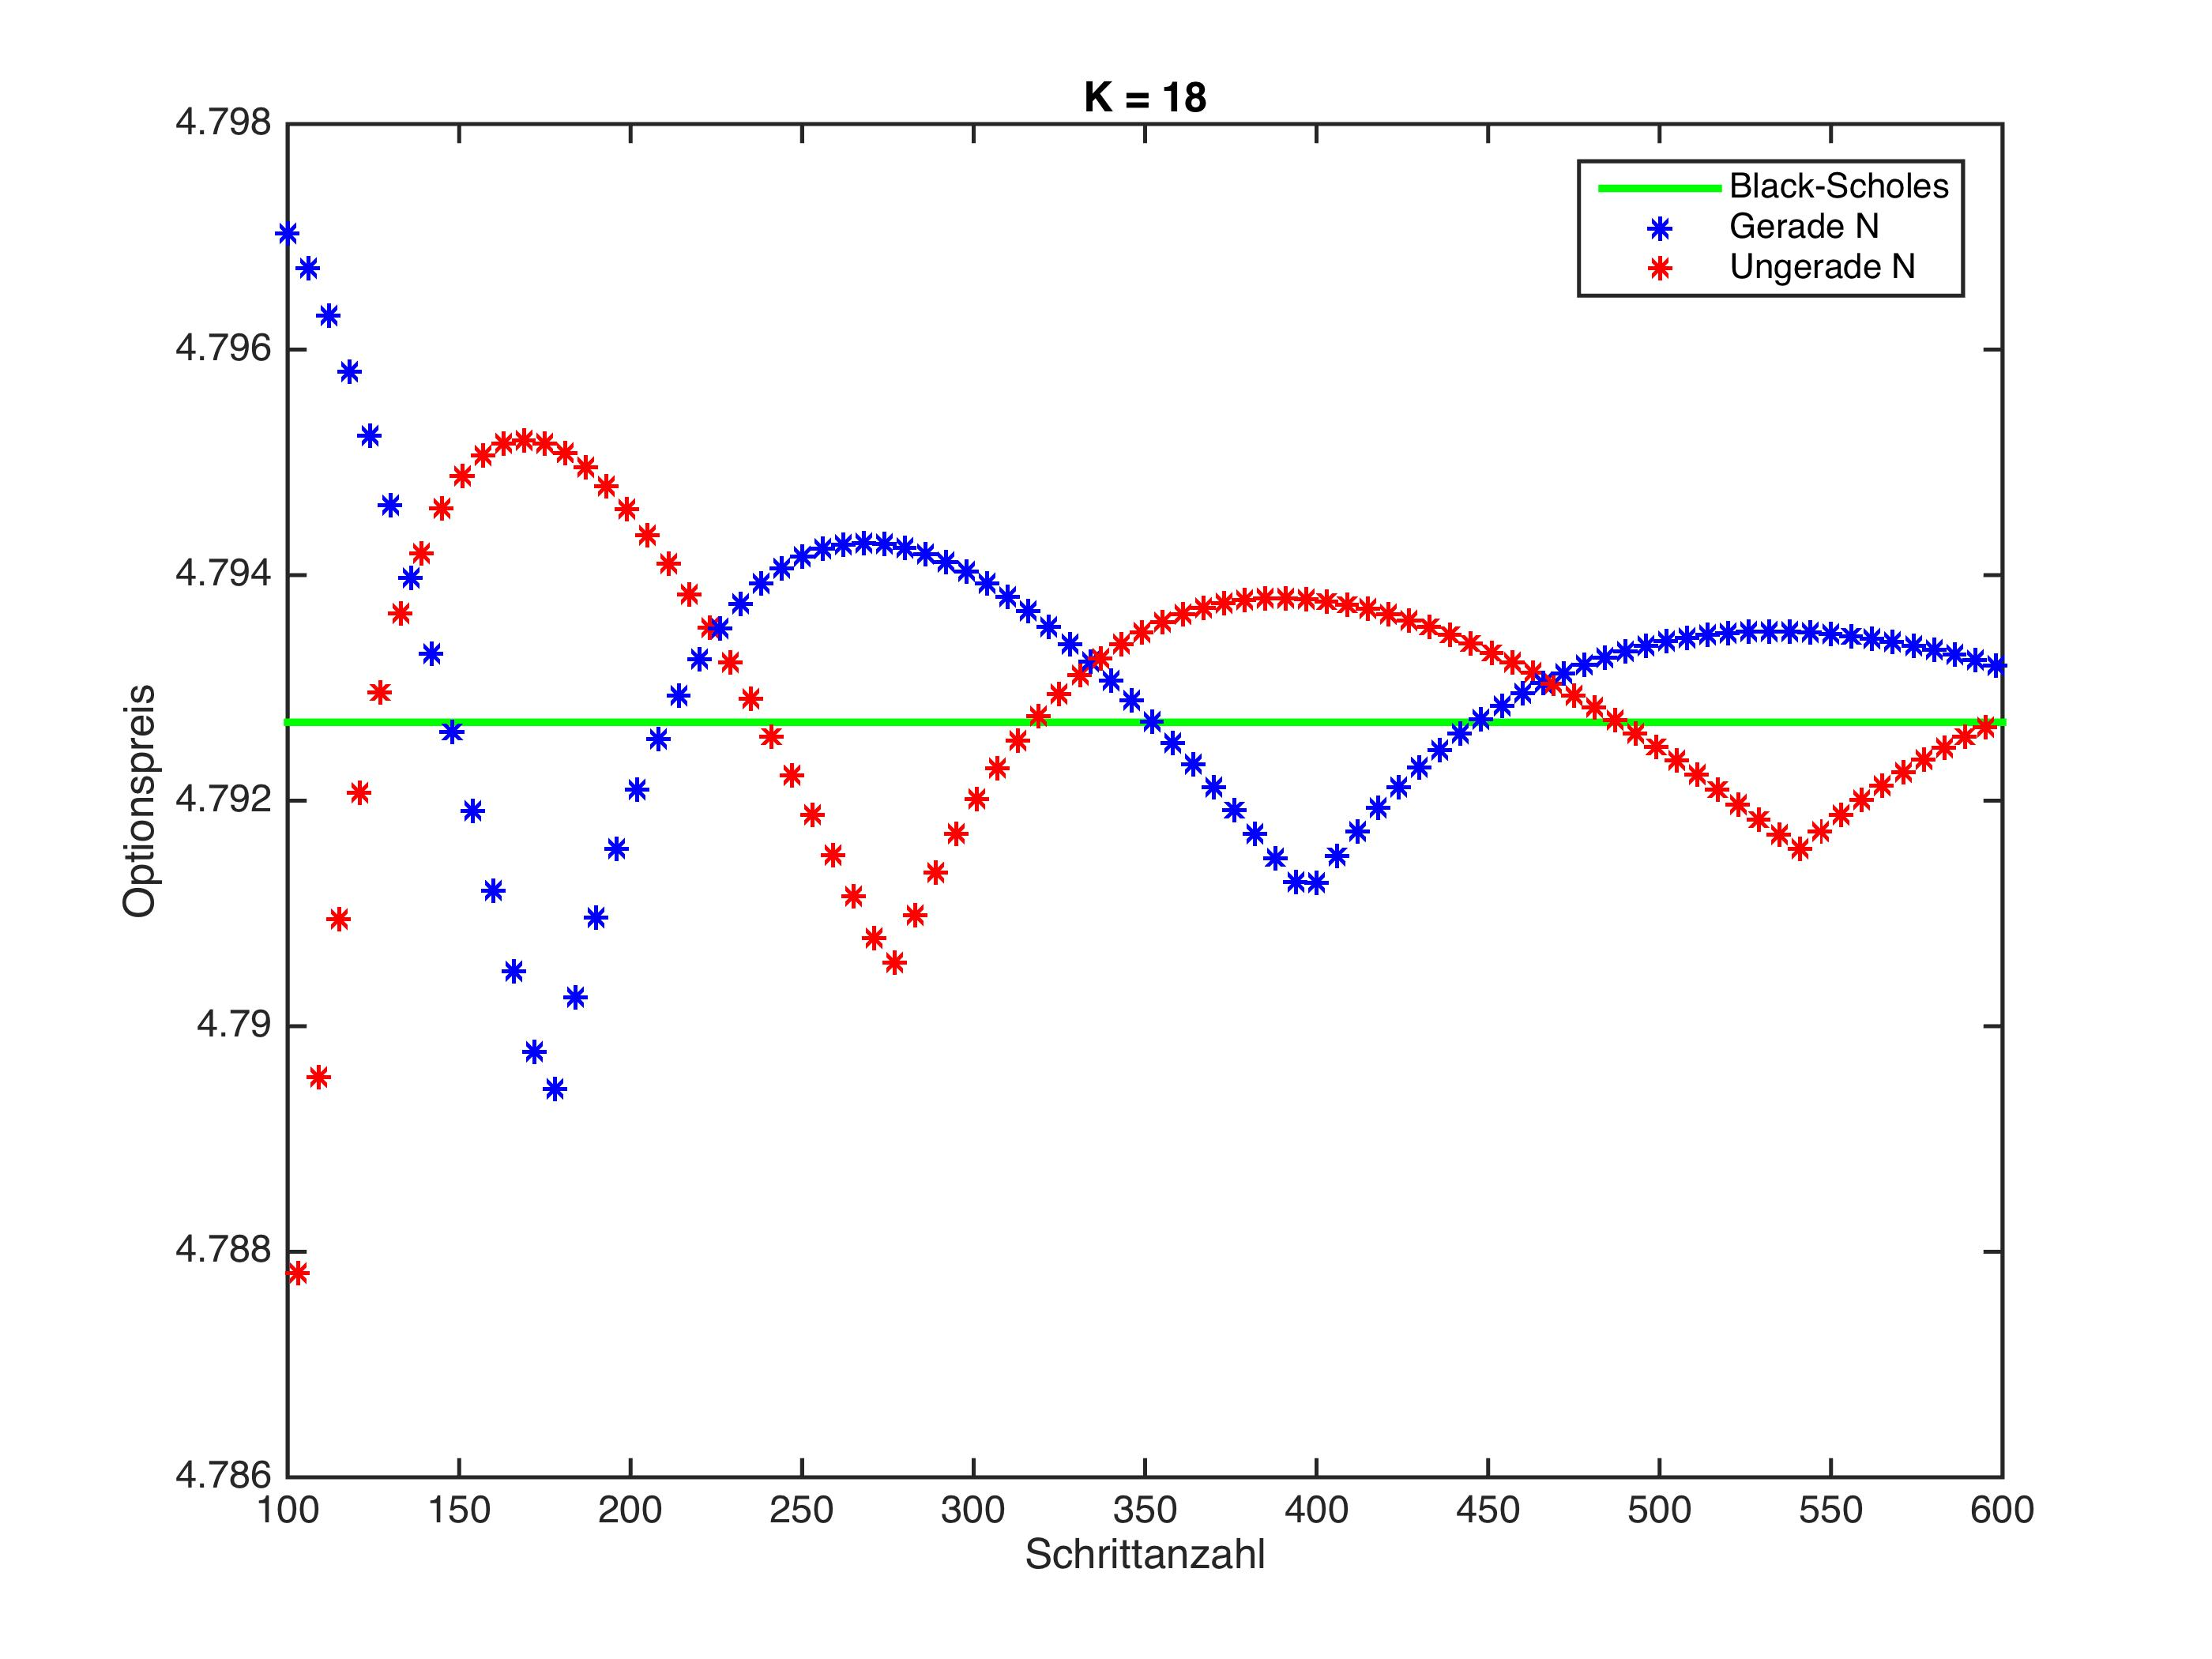
\includegraphics[width=0.45\textwidth]{KonvergenzCall18.jpg}
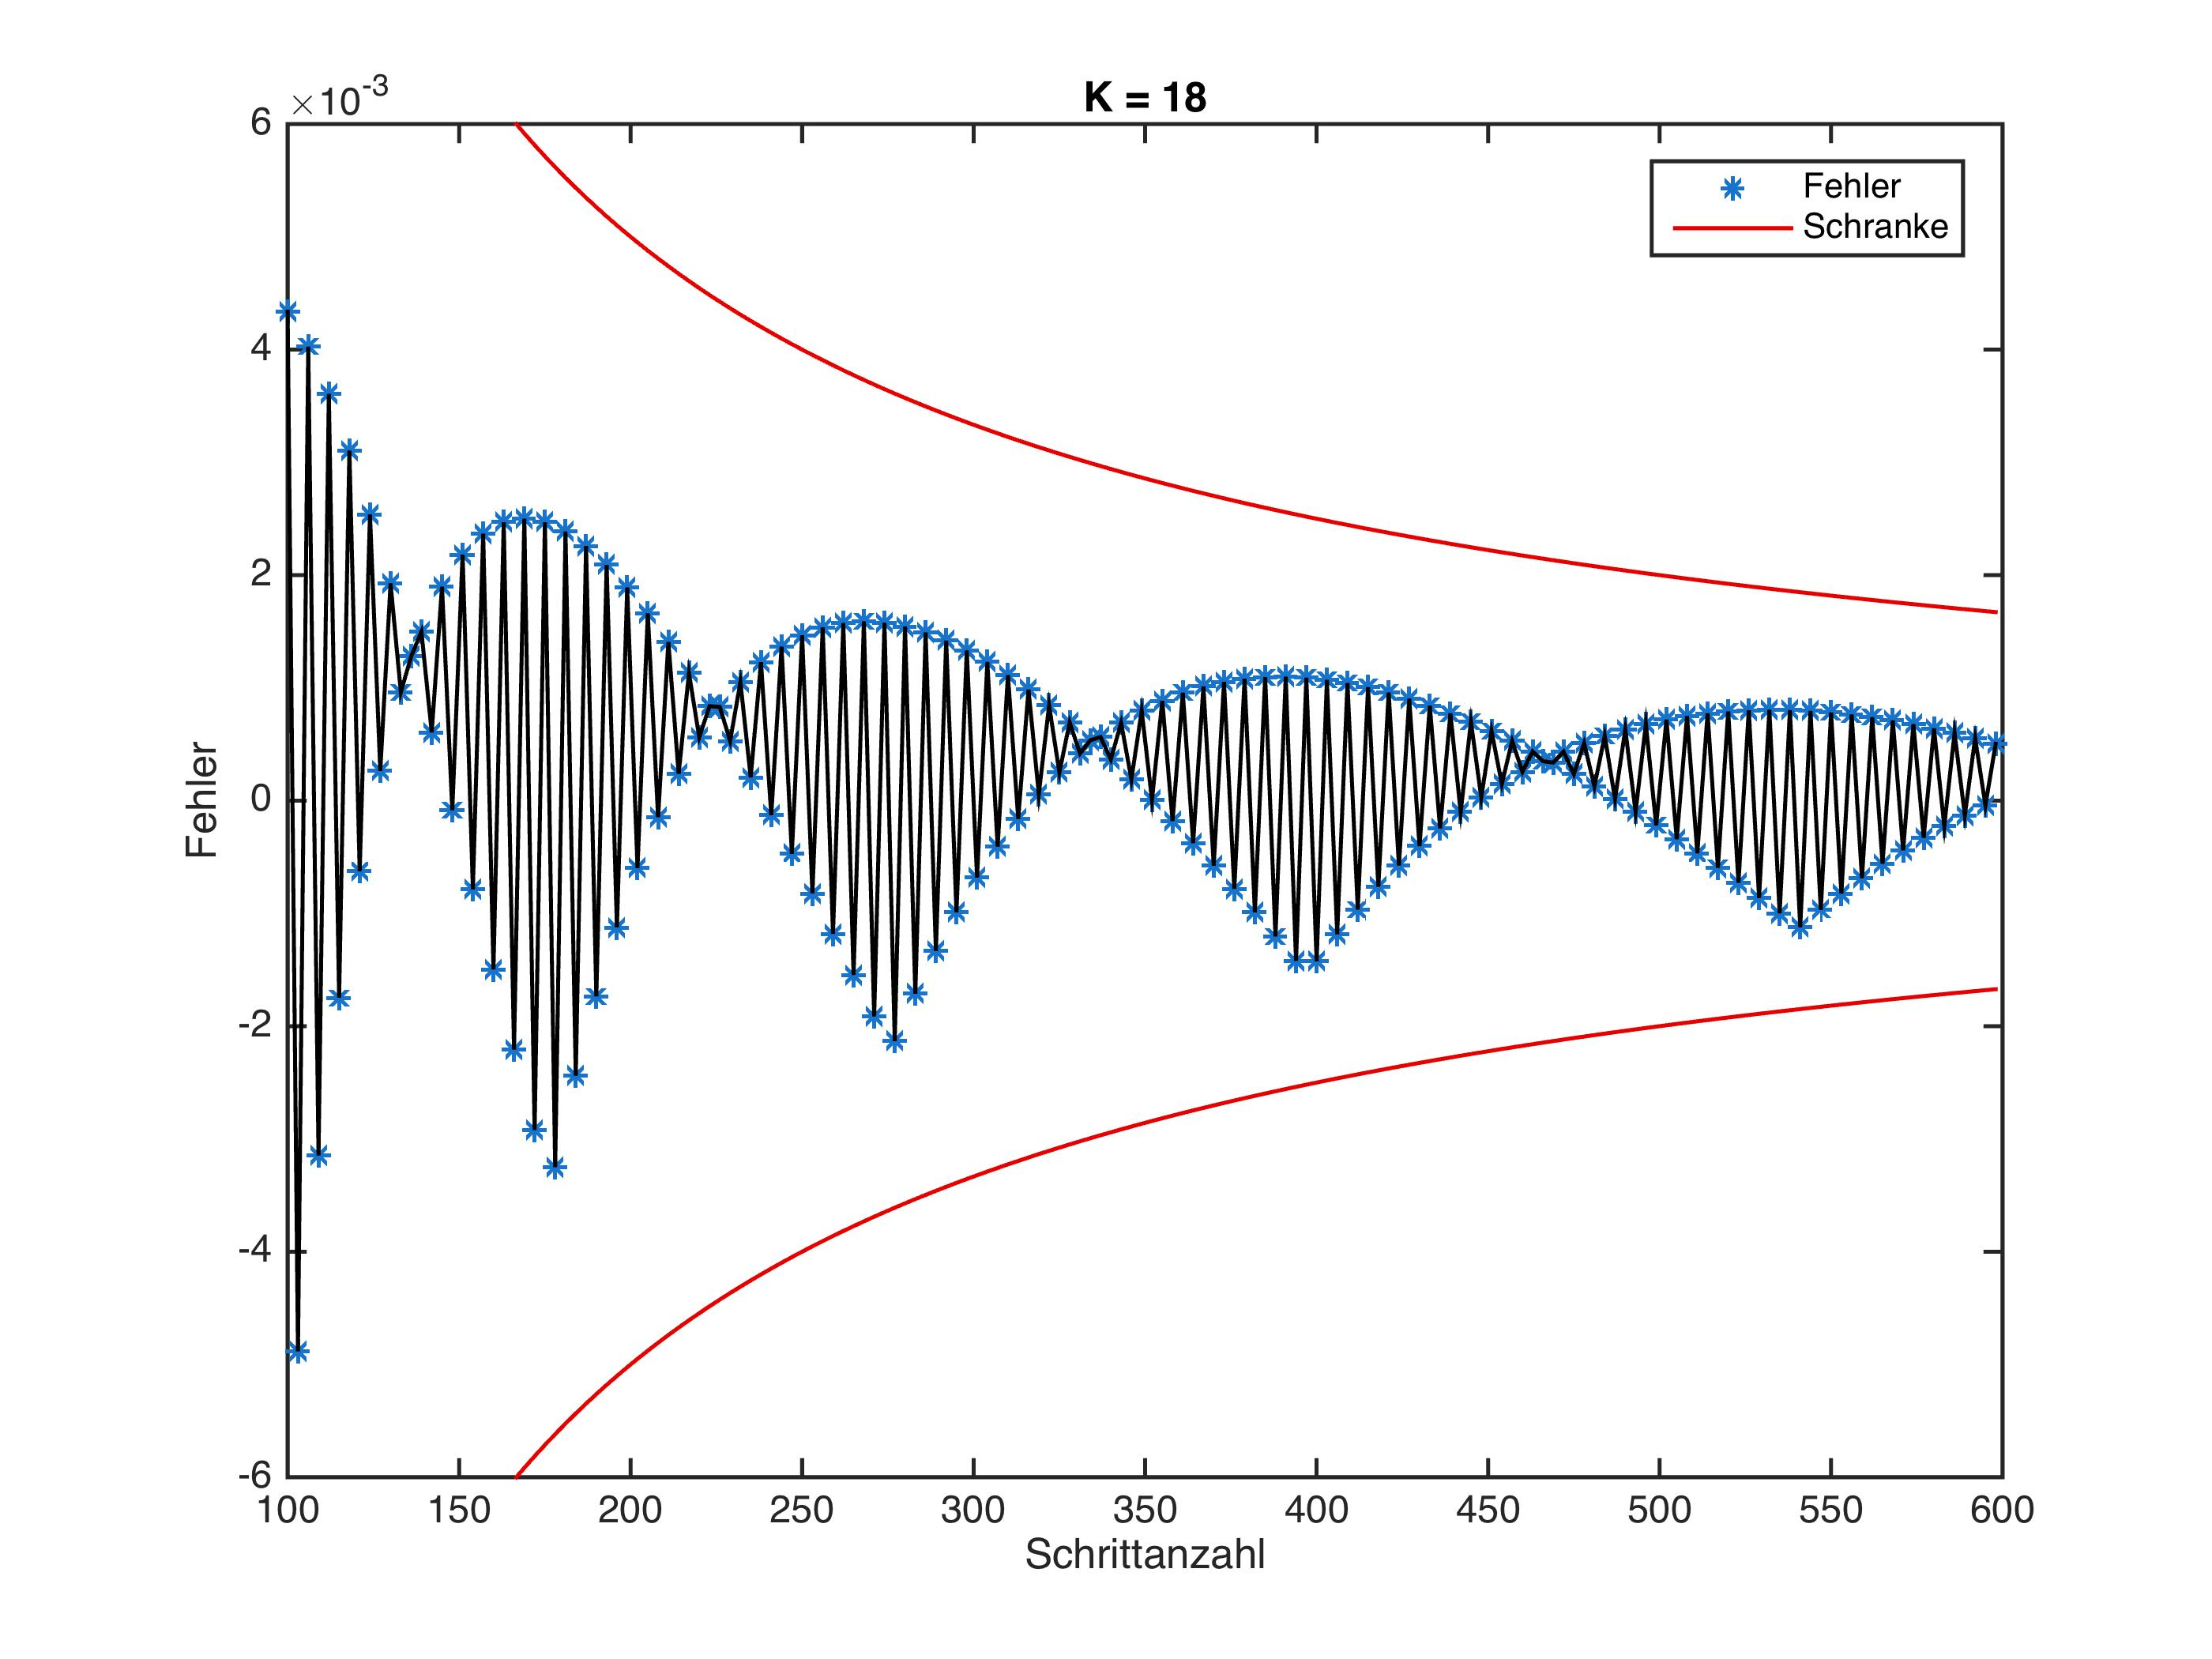
\includegraphics[width=0.45\textwidth]{FehlerCall18.jpg} \\
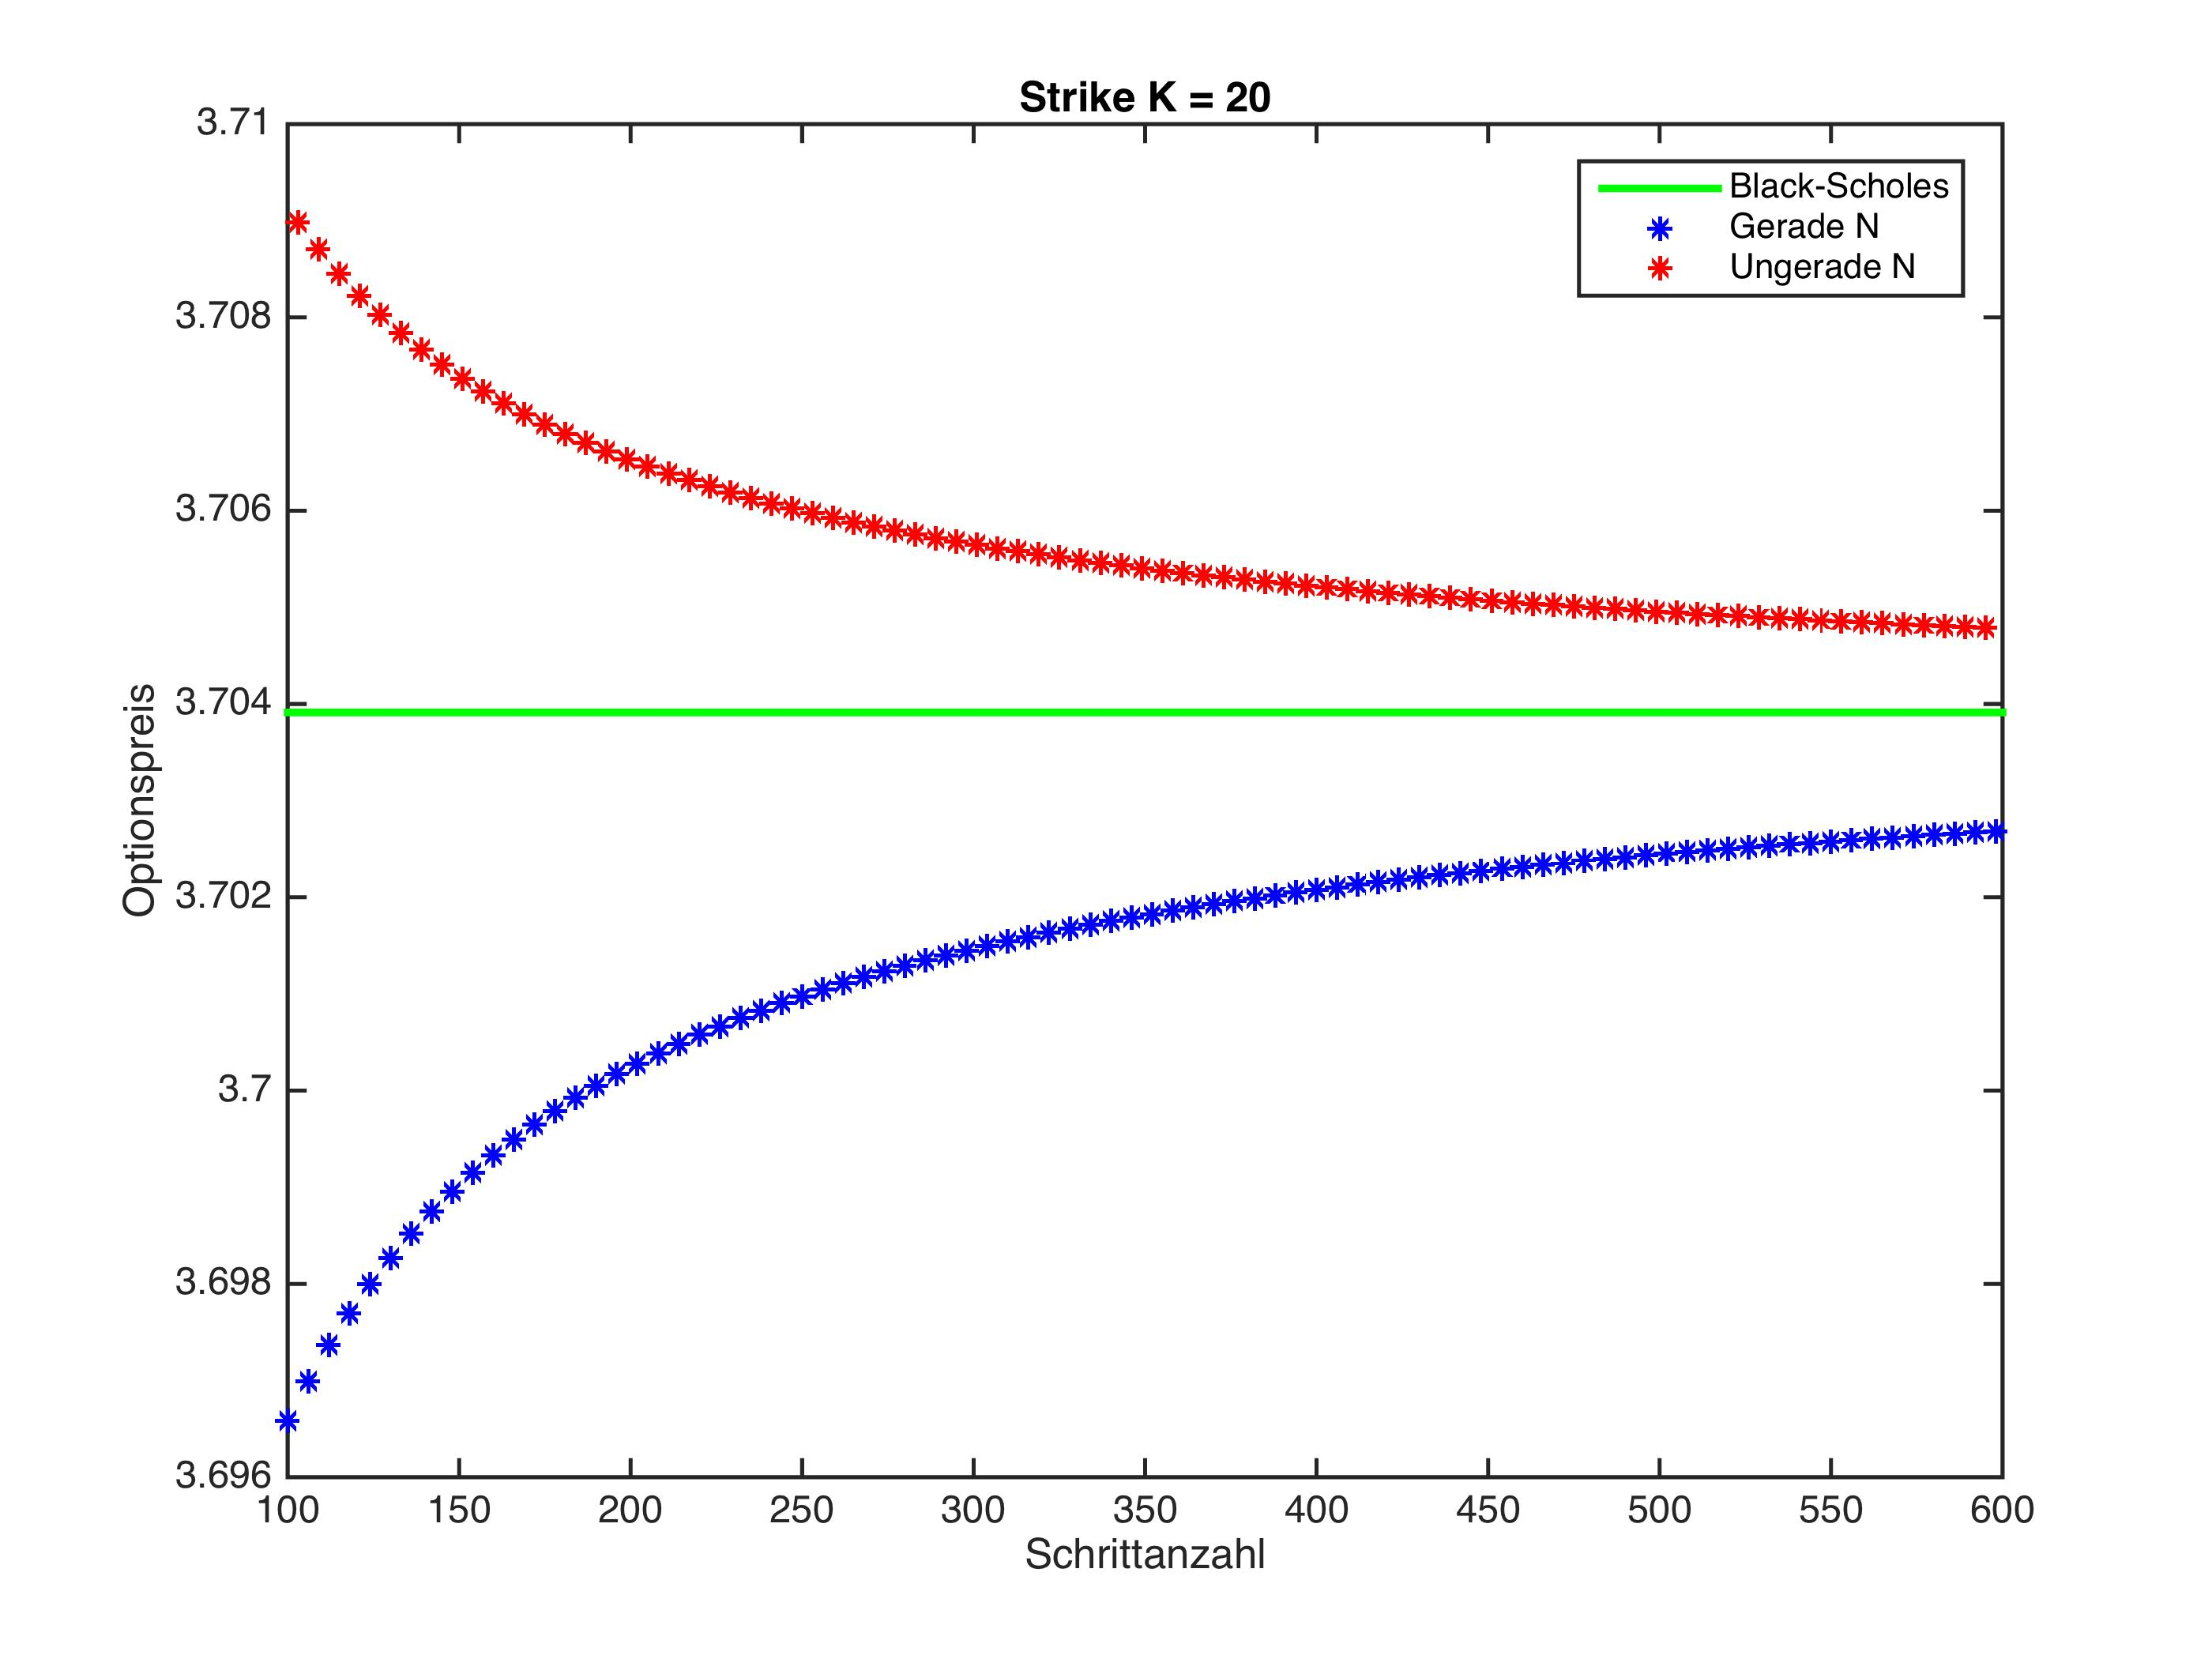
\includegraphics[width=0.45\textwidth]{KonvergenzCall20.jpg}
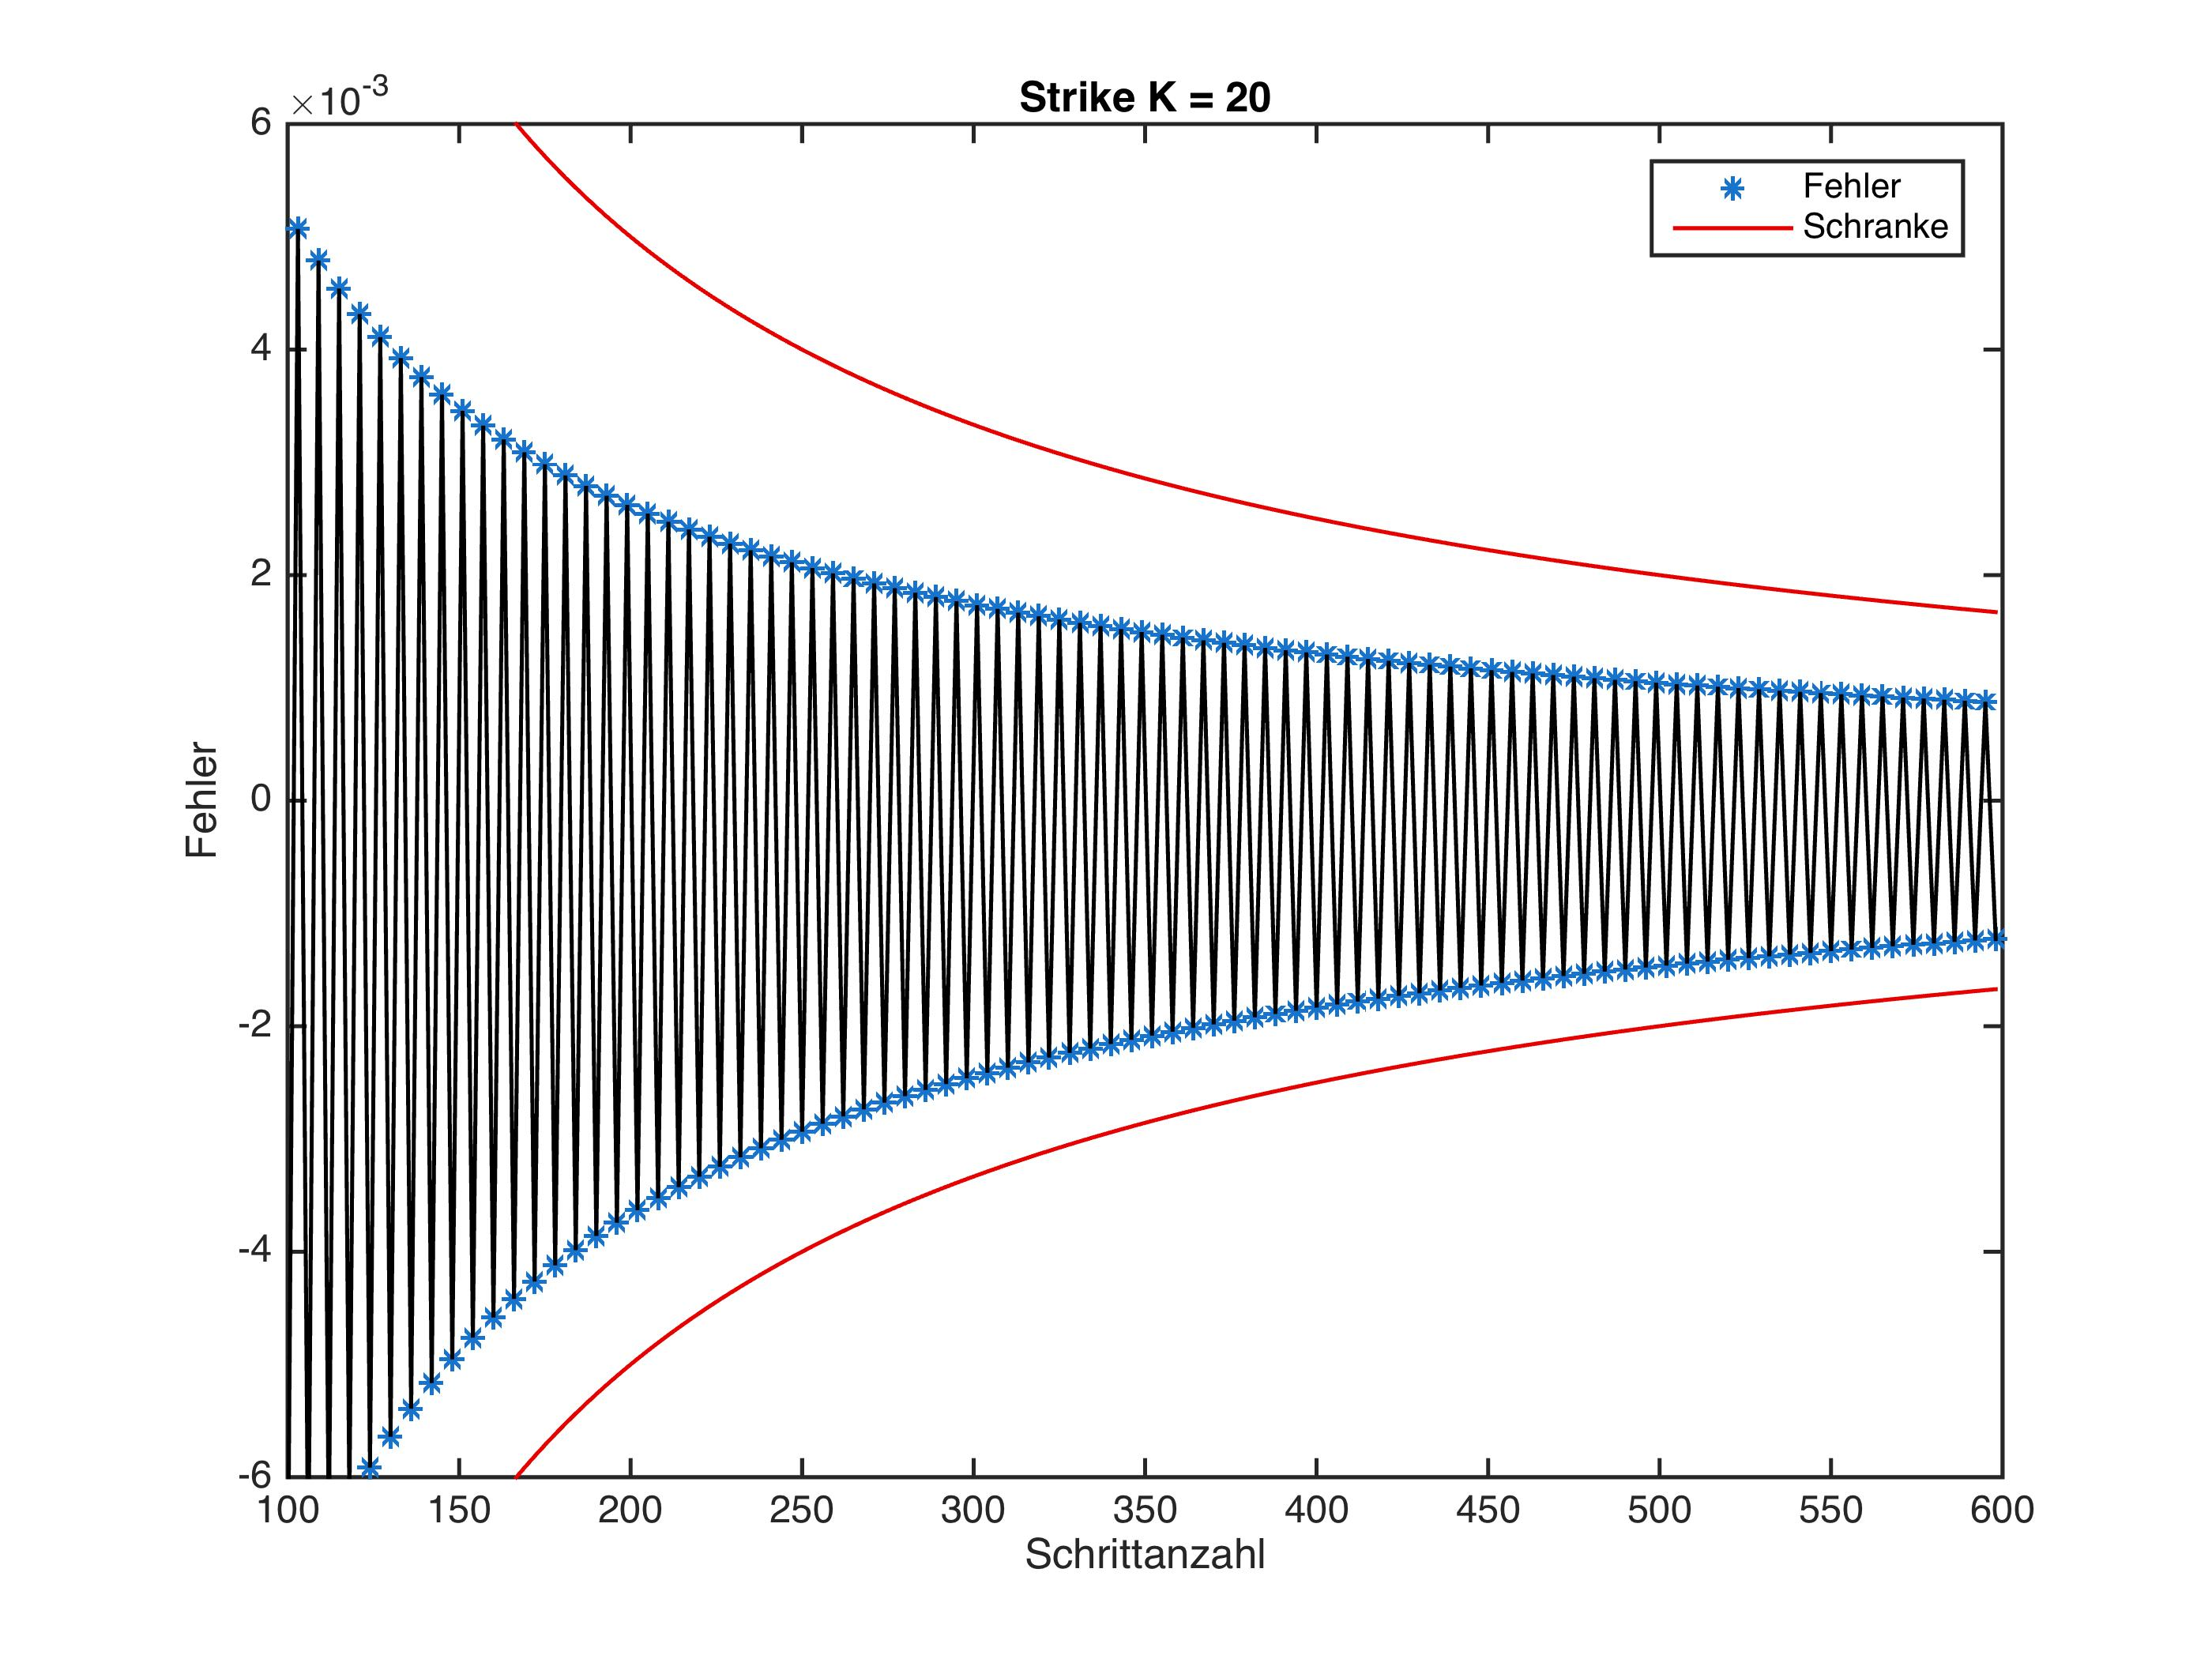
\includegraphics[width=0.45\textwidth]{FehlerCall20.jpg}
\caption{Konvergenz und Fehlerdarstellung für eine Europäische Call-Option mit $K=18$ bzw. $K=20$, $S_0=20$, $r = 0.1$, $\sigma = 0.35$ und $T=1$. Die Fehlerschranke ist $\frac{1}{N}$.}
\end{figure}\\
Was sofort auffällt, ist die unterschiedliche Konvergenz für die verschiedenen $K$. Während wir für $K=20$ eine jeweils monotone Konvergenz für gerade und ungerade Schrittanzahlen, sieht man für $K=18$ eine Art \glqq sprunghafte\grqq\, Konvergenz. Da $u_n$ und $d_n$ gegen $1$ konvergieren, konzentrieren sich immer mehr finale Knoten des Binomialbaums um $S_0$. 
\begin{figure}[h]
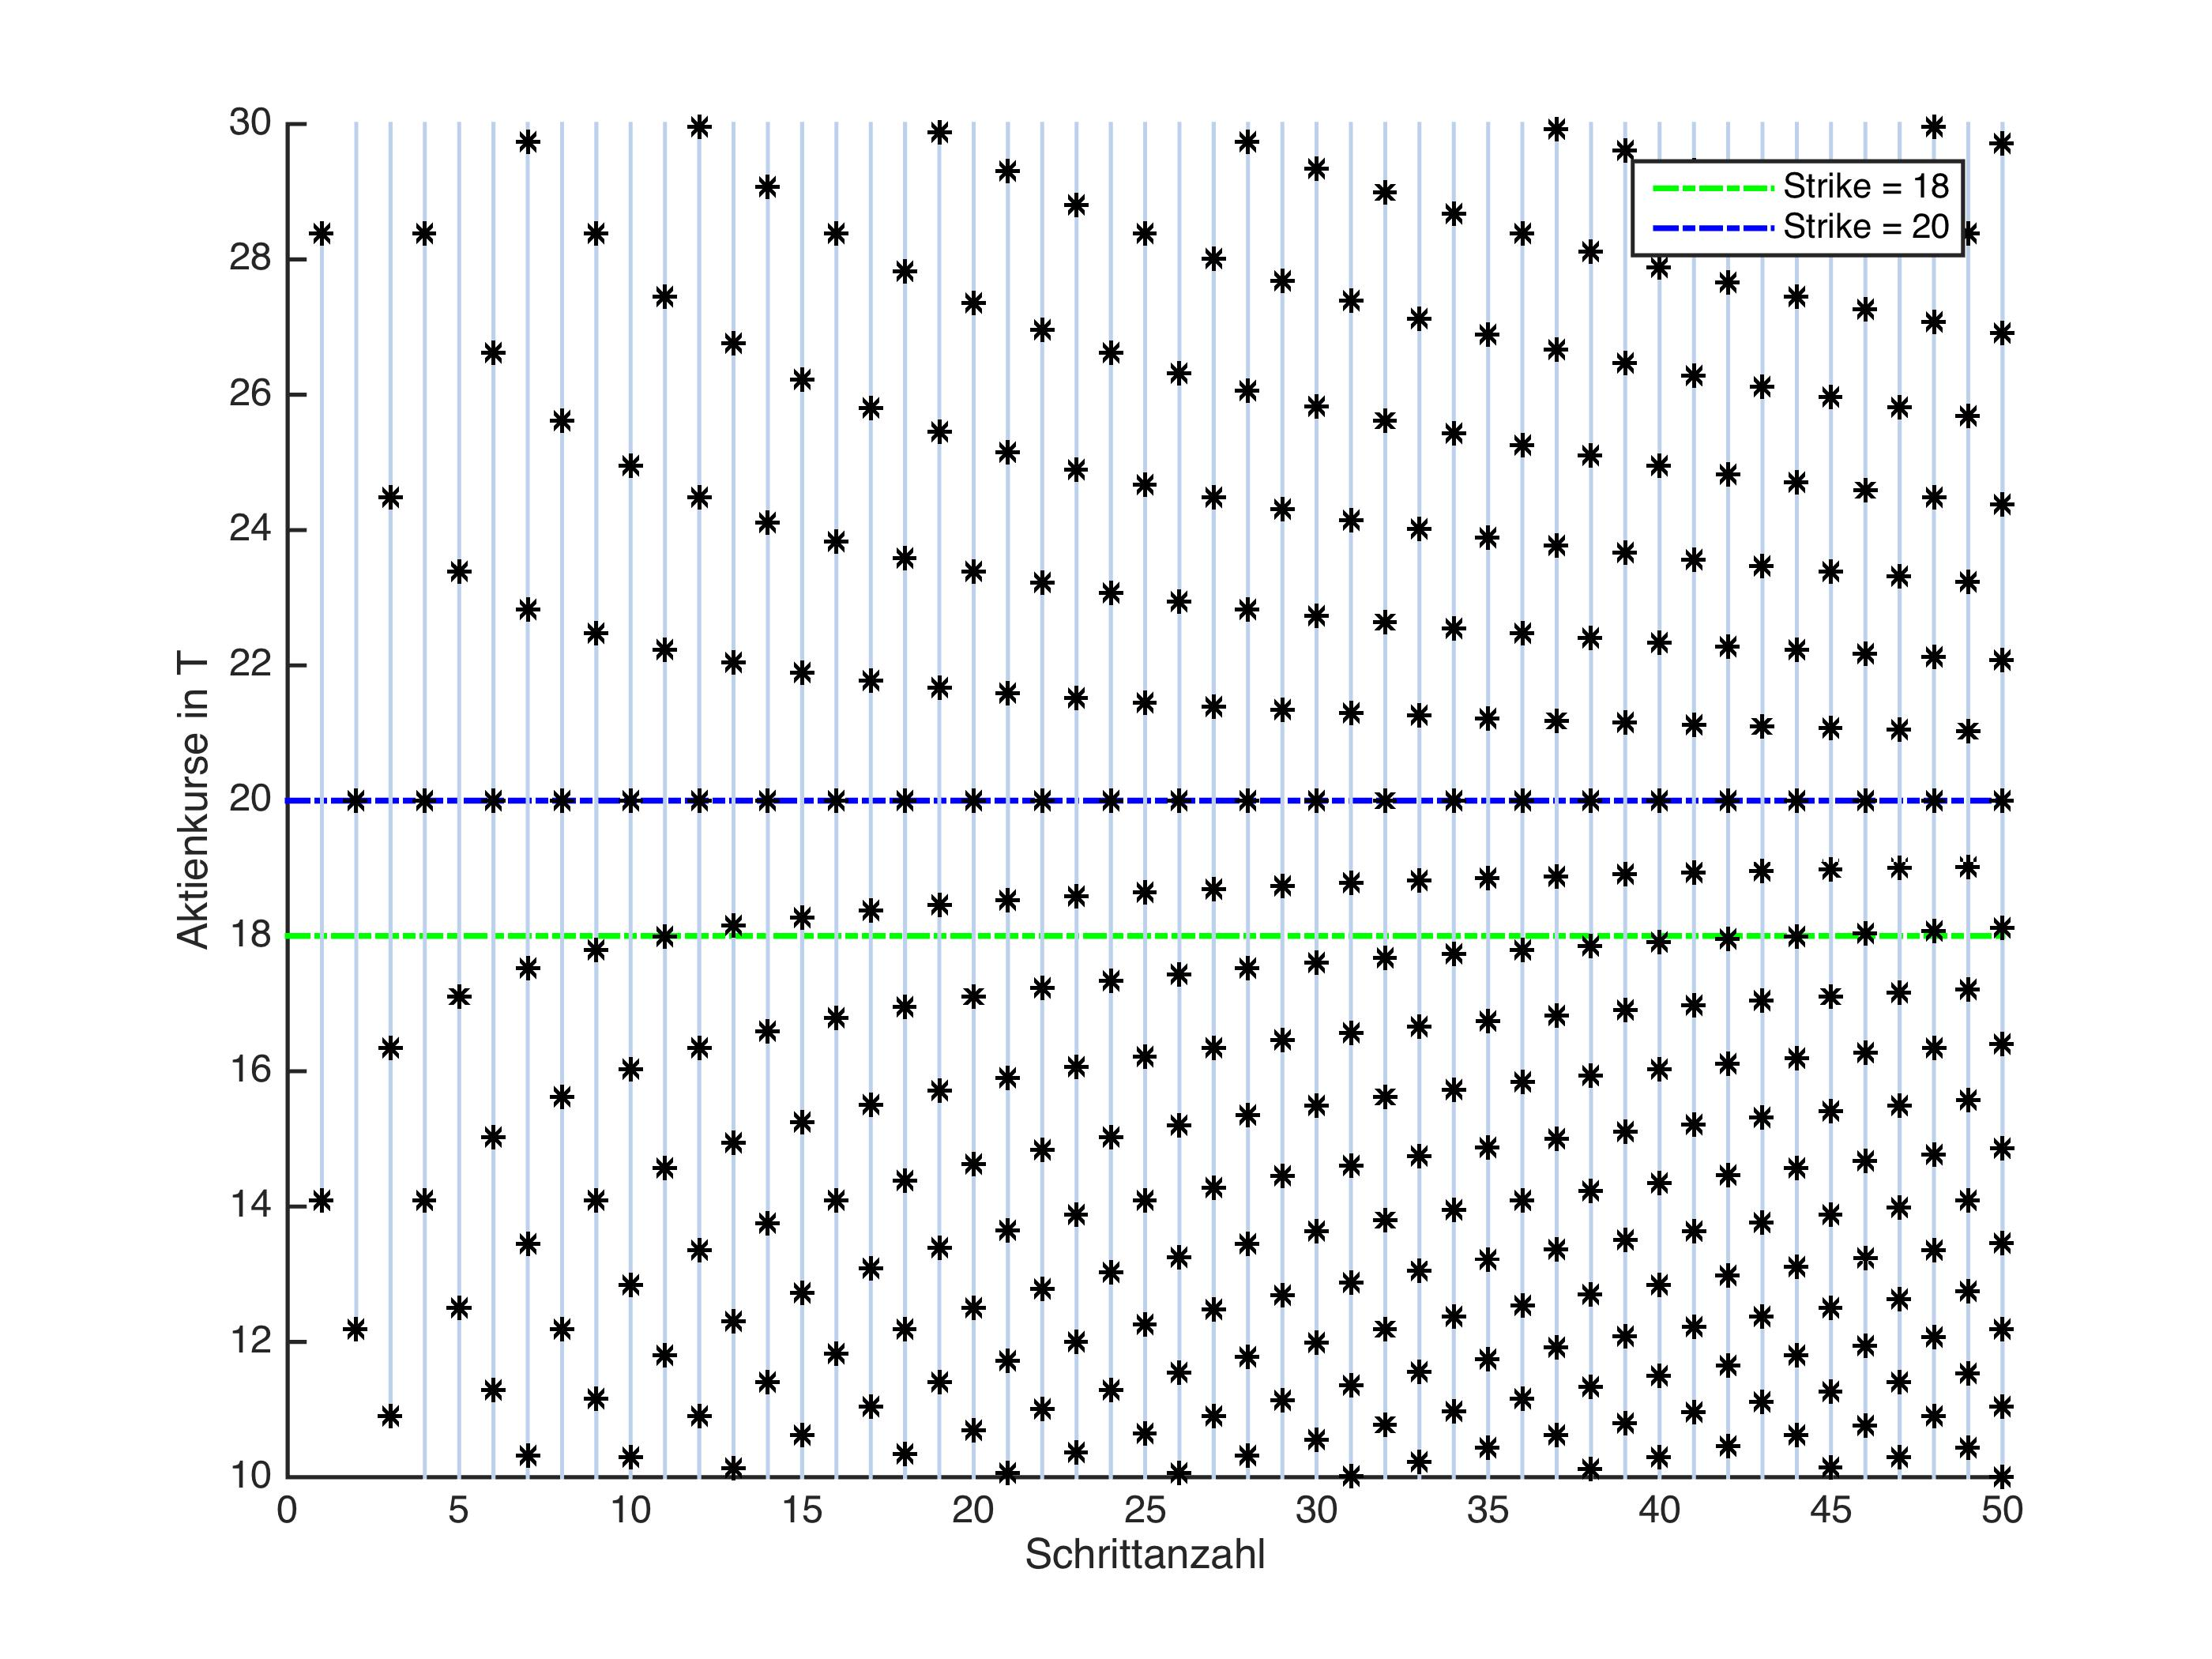
\includegraphics[width=0.9\textwidth]{Verjuengung.jpg}
\caption{Verjüngung der Endknoten in $T$ mit steigender Schrittanzahl.}
\end{figure}

Durch diese Verjüngung alterniert der Abstand des Strike Price $K=18$ zum nächsten Knoten im Endzeitpunkt $T$, wodurch die Sprünge in der Konvergenz erklärt werden \cite{LeisenReimer}. Je größer dabei der Abstand ist, desto mehr wird die Option überbewertet. Wenn $K=S_0$, so liegt wegen $u\cdot d = 1$ der Strike Price für gerade $N$ genau auf einem finalen Knoten und für ungerade $N$ genau zwischen zwei Knoten, was die jeweils monotone Konvergenz für $K=20$ erklärt.


%%%%%%%%% BLACK SCHOLES BEISPIELE %%%%%%%%%%%%%%%%%%%%%%%
\newpage
\section{Black-Scholes-Modell}
\label{BSP:BSModell}
Im Folgenden sind jeweils die Werte einer Put- und einer Call-Option im Vergleich zwischen Europäischer und Amerikanischer Version geplottet. 
\begin{figure}[h]
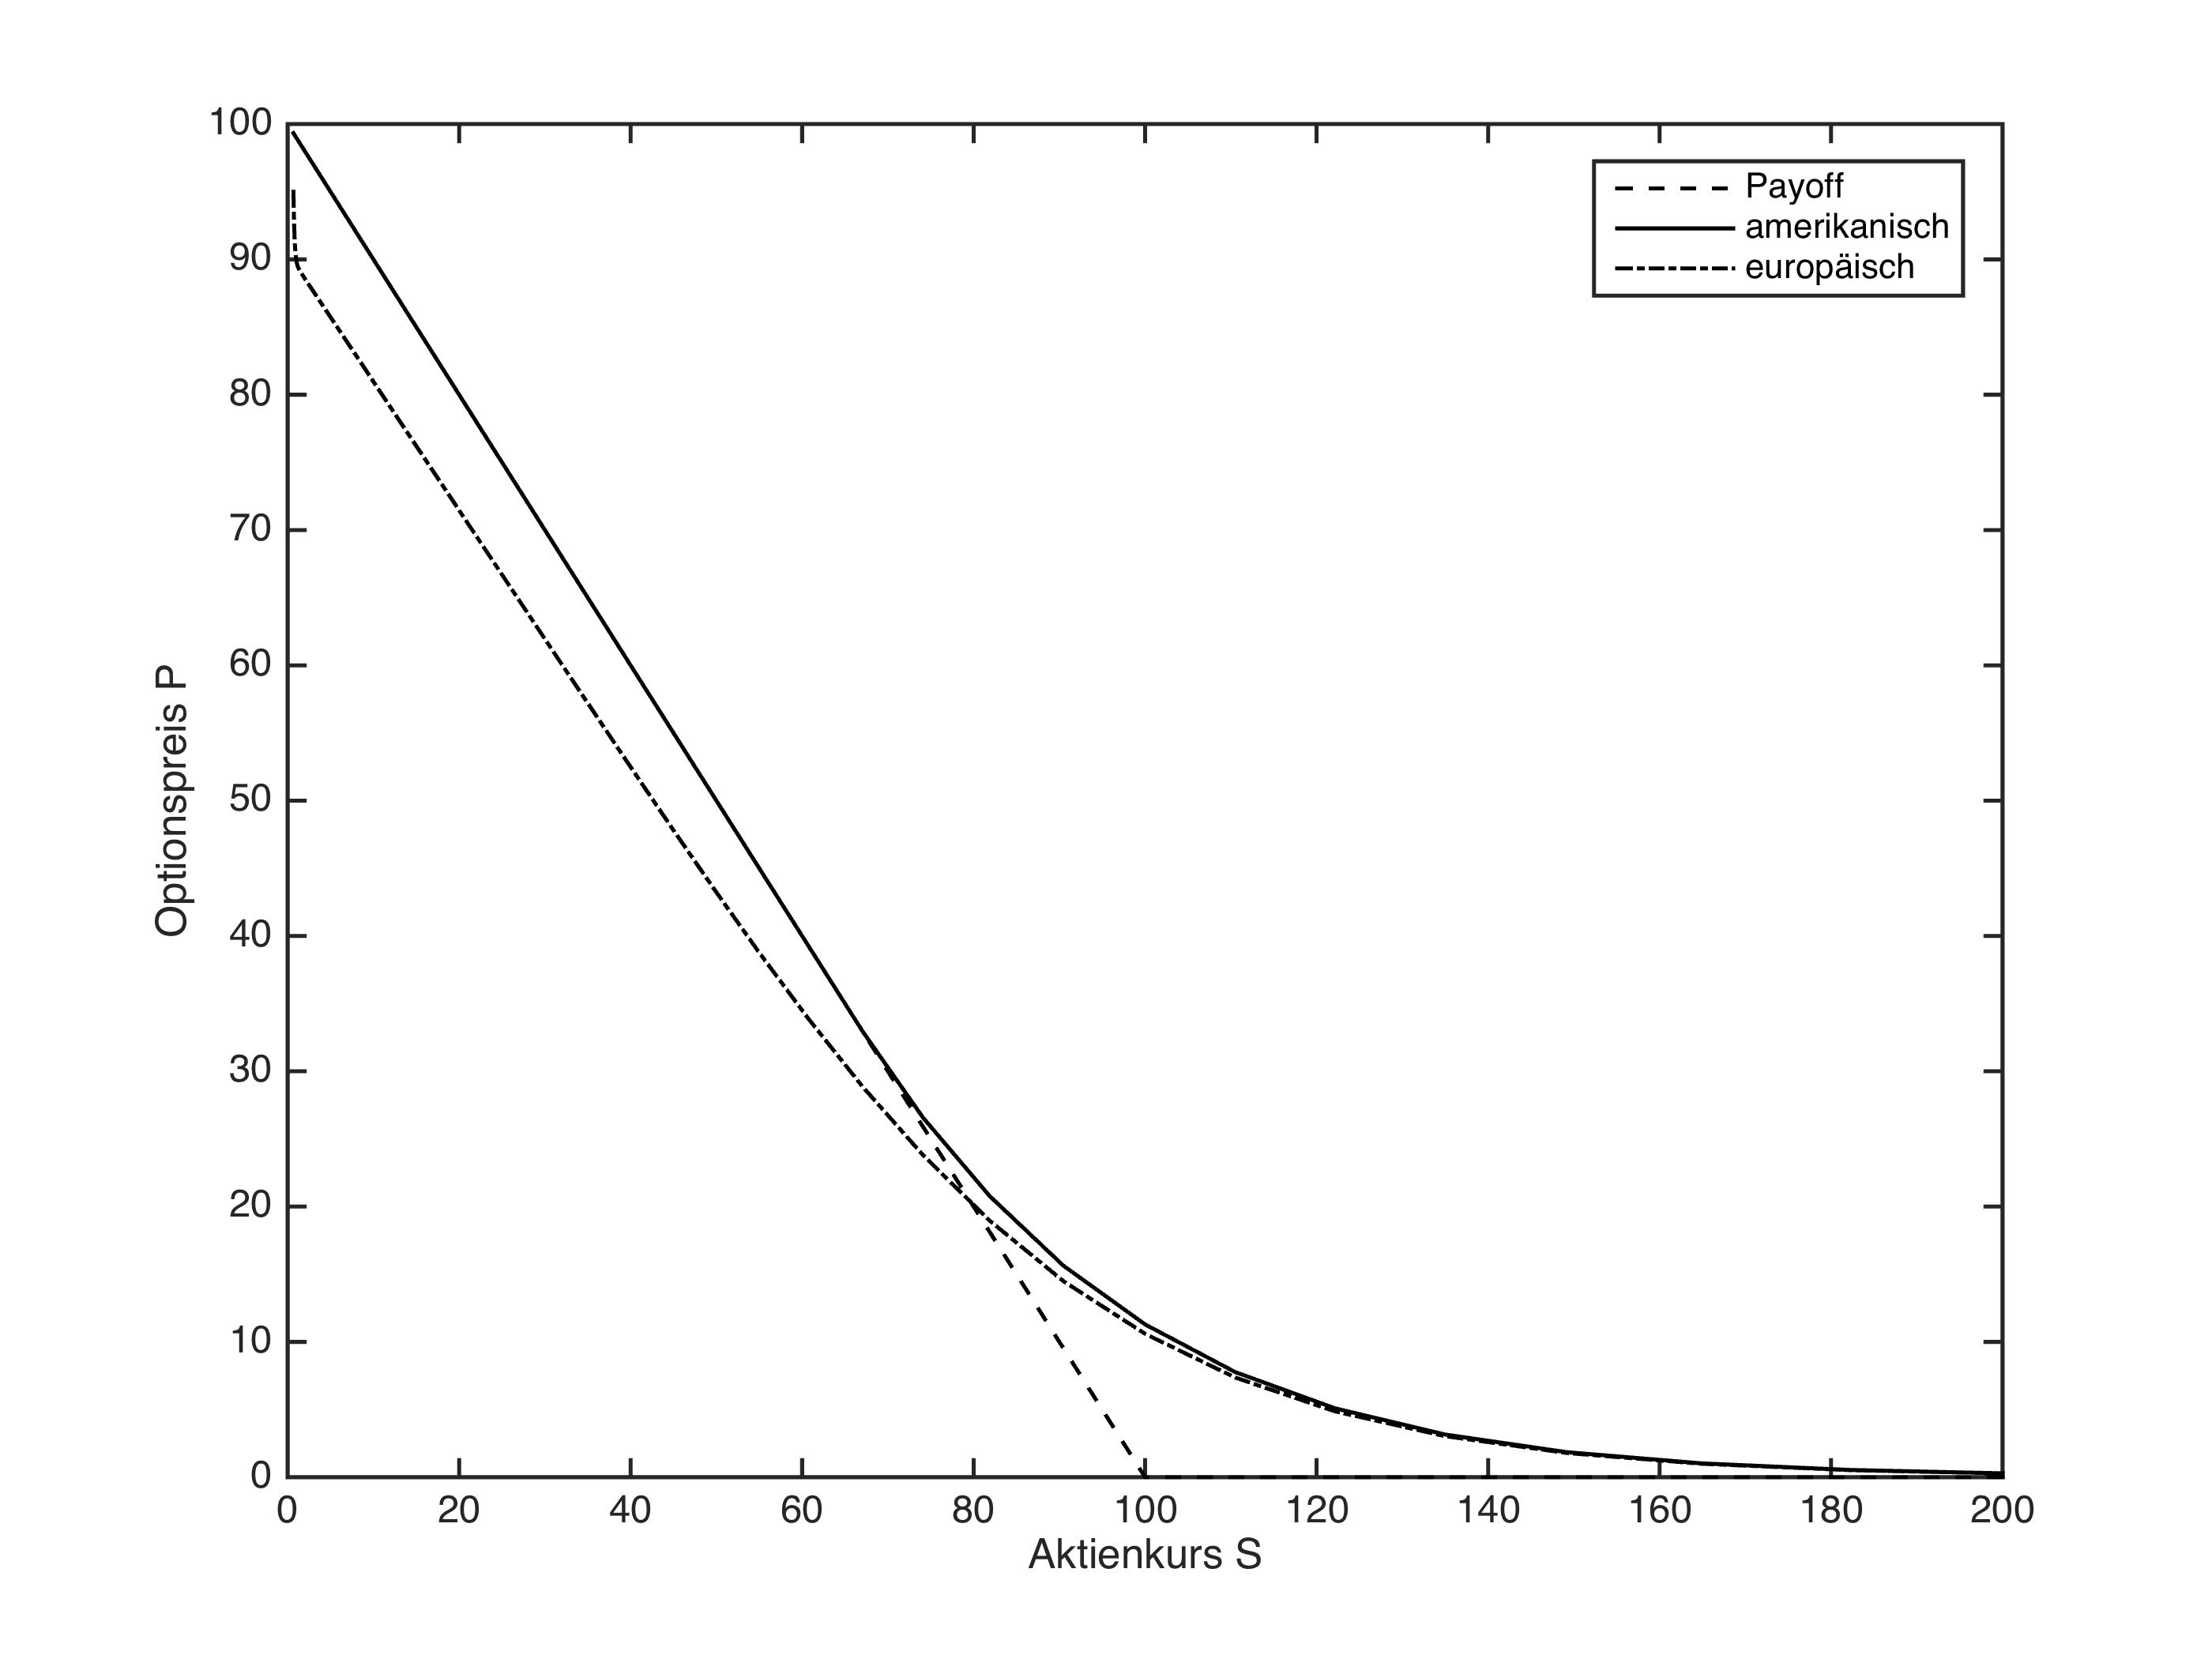
\includegraphics[width=0.9\textwidth]{PlotPutOption.jpg}
\caption{Wert einer Europäischen und einer Amerikanischen Put-Option mit $r = 0.1$, $\sigma^2 = 0.35$, $T=1$ und $D_0 = 0.05$. Berechnet durch Diskretisierung der Wärmeleitungsgleichung mit $a=5$, $M=5$ und $N=100$.}
\end{figure}
Man sieht direkt, dass der Wert der Amerikanischen Option immer größer ist als der der Europäischen. Es ist zu erkennen, dass sich die Optionswerte nicht nur in den Aktienkursen, zu denen eine Ausübung sinnvoll wäre, unterscheiden, sondern auch danach bzw. davor. Dies erscheint auch plausibel, da es für einen Aktienkurs nahe der Ausübungsgrenze wahrscheinlich ist, dass vom frühzeitigen Ausübungsrecht der Amerikanischen Option gebraucht gemacht wird. Diese Grenze, den im Komplementaritätsproblem (\ref{BS:LKP1})-(\ref{BS:LKP3}) implizit formulierten freien Randwert $S_f(t)$, kann man im Schaubild der Optionswerte nur schwer ablesen, allderdings lässt er sich innerhalb der Matlab Funktion durch Vergleich der Lösung $V(S_0,0)$ mit $\Lambda(S_0)$ mit geringem Aufwand ausgeben. Es gilt $S_f^p(0)\approx 74.0818$ für die Put-Option und $S_f^c(0) \approx 201.3753$. Die Approximation von $S_f^c$ ist allerdings kritisch zu betrachten, da die Gitterpunkte durch die gewählte Approximation für $S>K$ einen sehr großen Abstand haben. 
\begin{figure}[h]
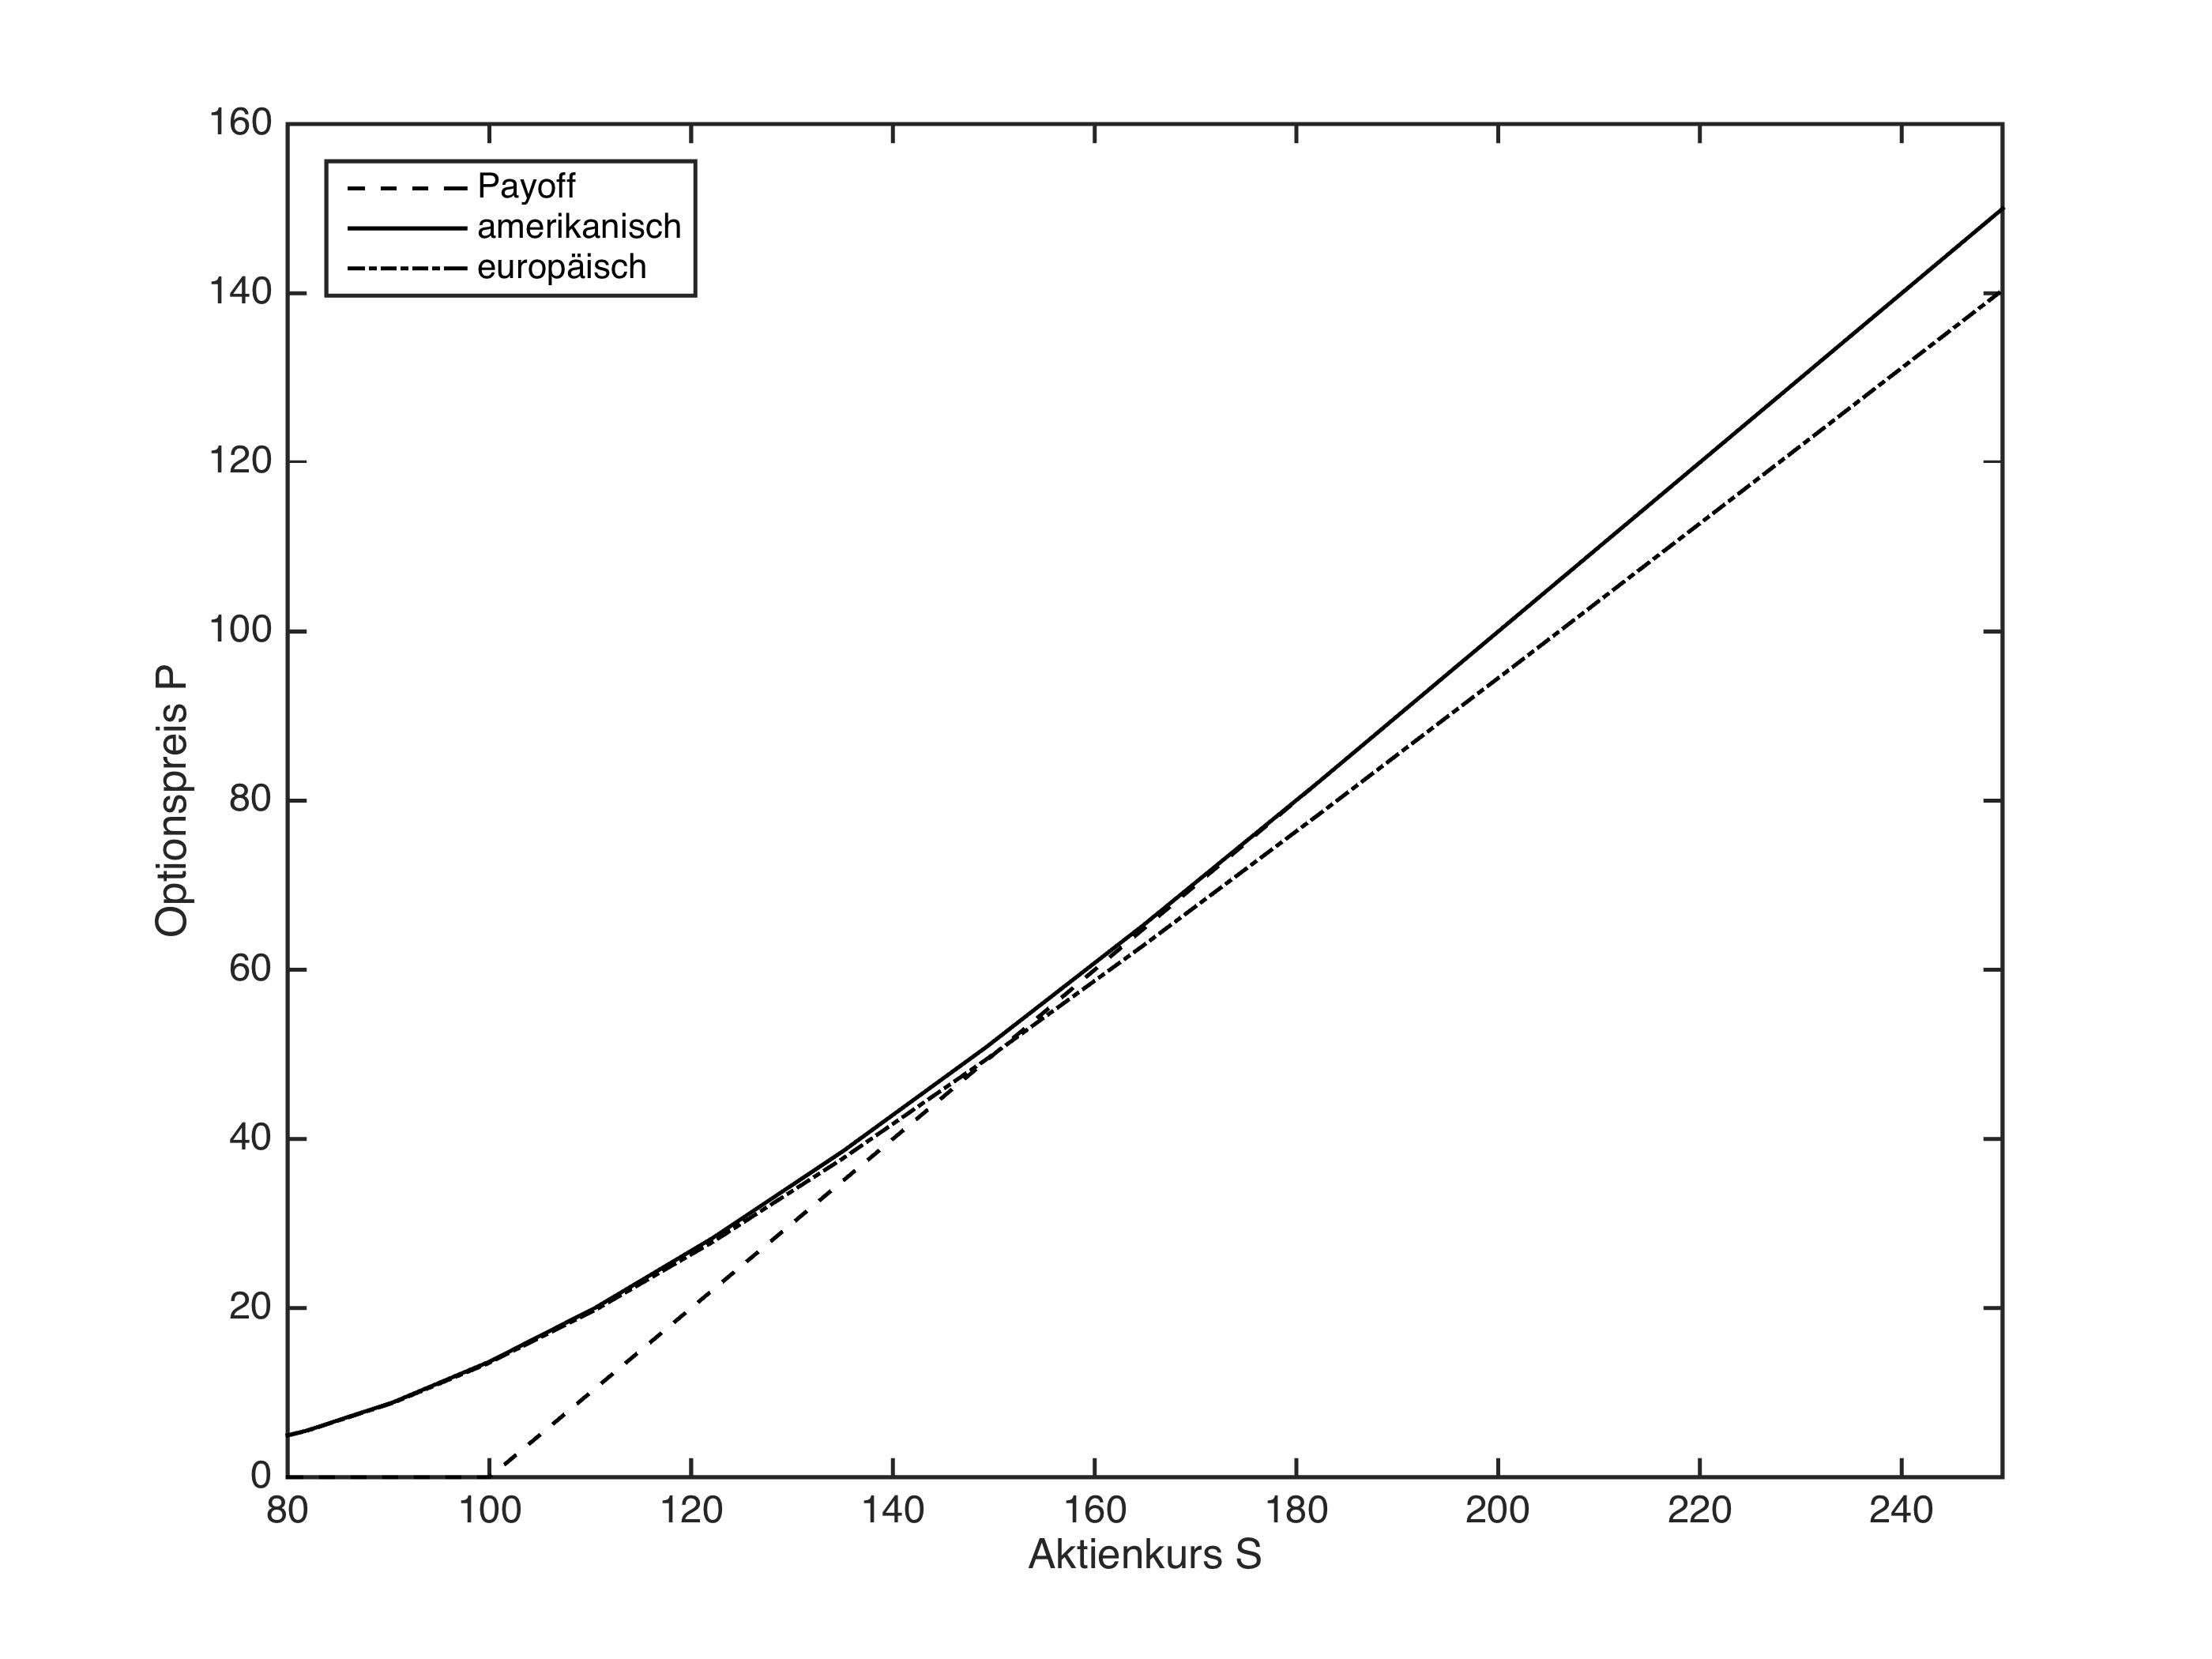
\includegraphics[width=0.9\textwidth]{PlotCallOption.jpg}
\caption{Wert einer Europäischen und einer Amerikanischen Call-Option mit $r = 0.1$, $\sigma^2 = 0.35$, $T=1$ und $D_0 = 0.08$. Berechnet durch Diskretisierung der Wärmeleitungsgleichung mit $a=5$, $M=5$ und $N=100$.}
\end{figure}
Möglichkeiten, die Approximation zu verbessern wären zum Einen eine Erhöhung der Schrittanzahl (was aber den Rechenaufwand und damit die Laufzeit stark erhöht), zum Anderen mithilfe eines aus dem Plot abgelesenen approximativen $S_f^c$ eine verbesserte Wahl des Gitters. Man kann dann zu gleicher Anzahl an Gitterpunkten die Diskretisierung z.B. nur auf $\left[-a,k\cdot a\right]$ (für geeignetes $k\in \left(0,1\right]$) durchführen und erhält damit eine feinere Darstellung für $K\leq S \leq S_f^c$. Mit $k=0.2$ erhalten wir $S_f^c \approx 185.8928$, was eine bessere Approximation an den \glqq wahren\grqq \, Randwert $\tilde S_f^c = 181.7387$ (berechnet mit $N=10\,000$ Gitterpunkten auf $\left[-a,0.2\cdot a\right]$) liefert.

%In der folgenden Abbildung lassen sich sowohl der in $t$ fallende freie Randwert $S_f(t)$, also auch die
%\begin{figure}[h]
%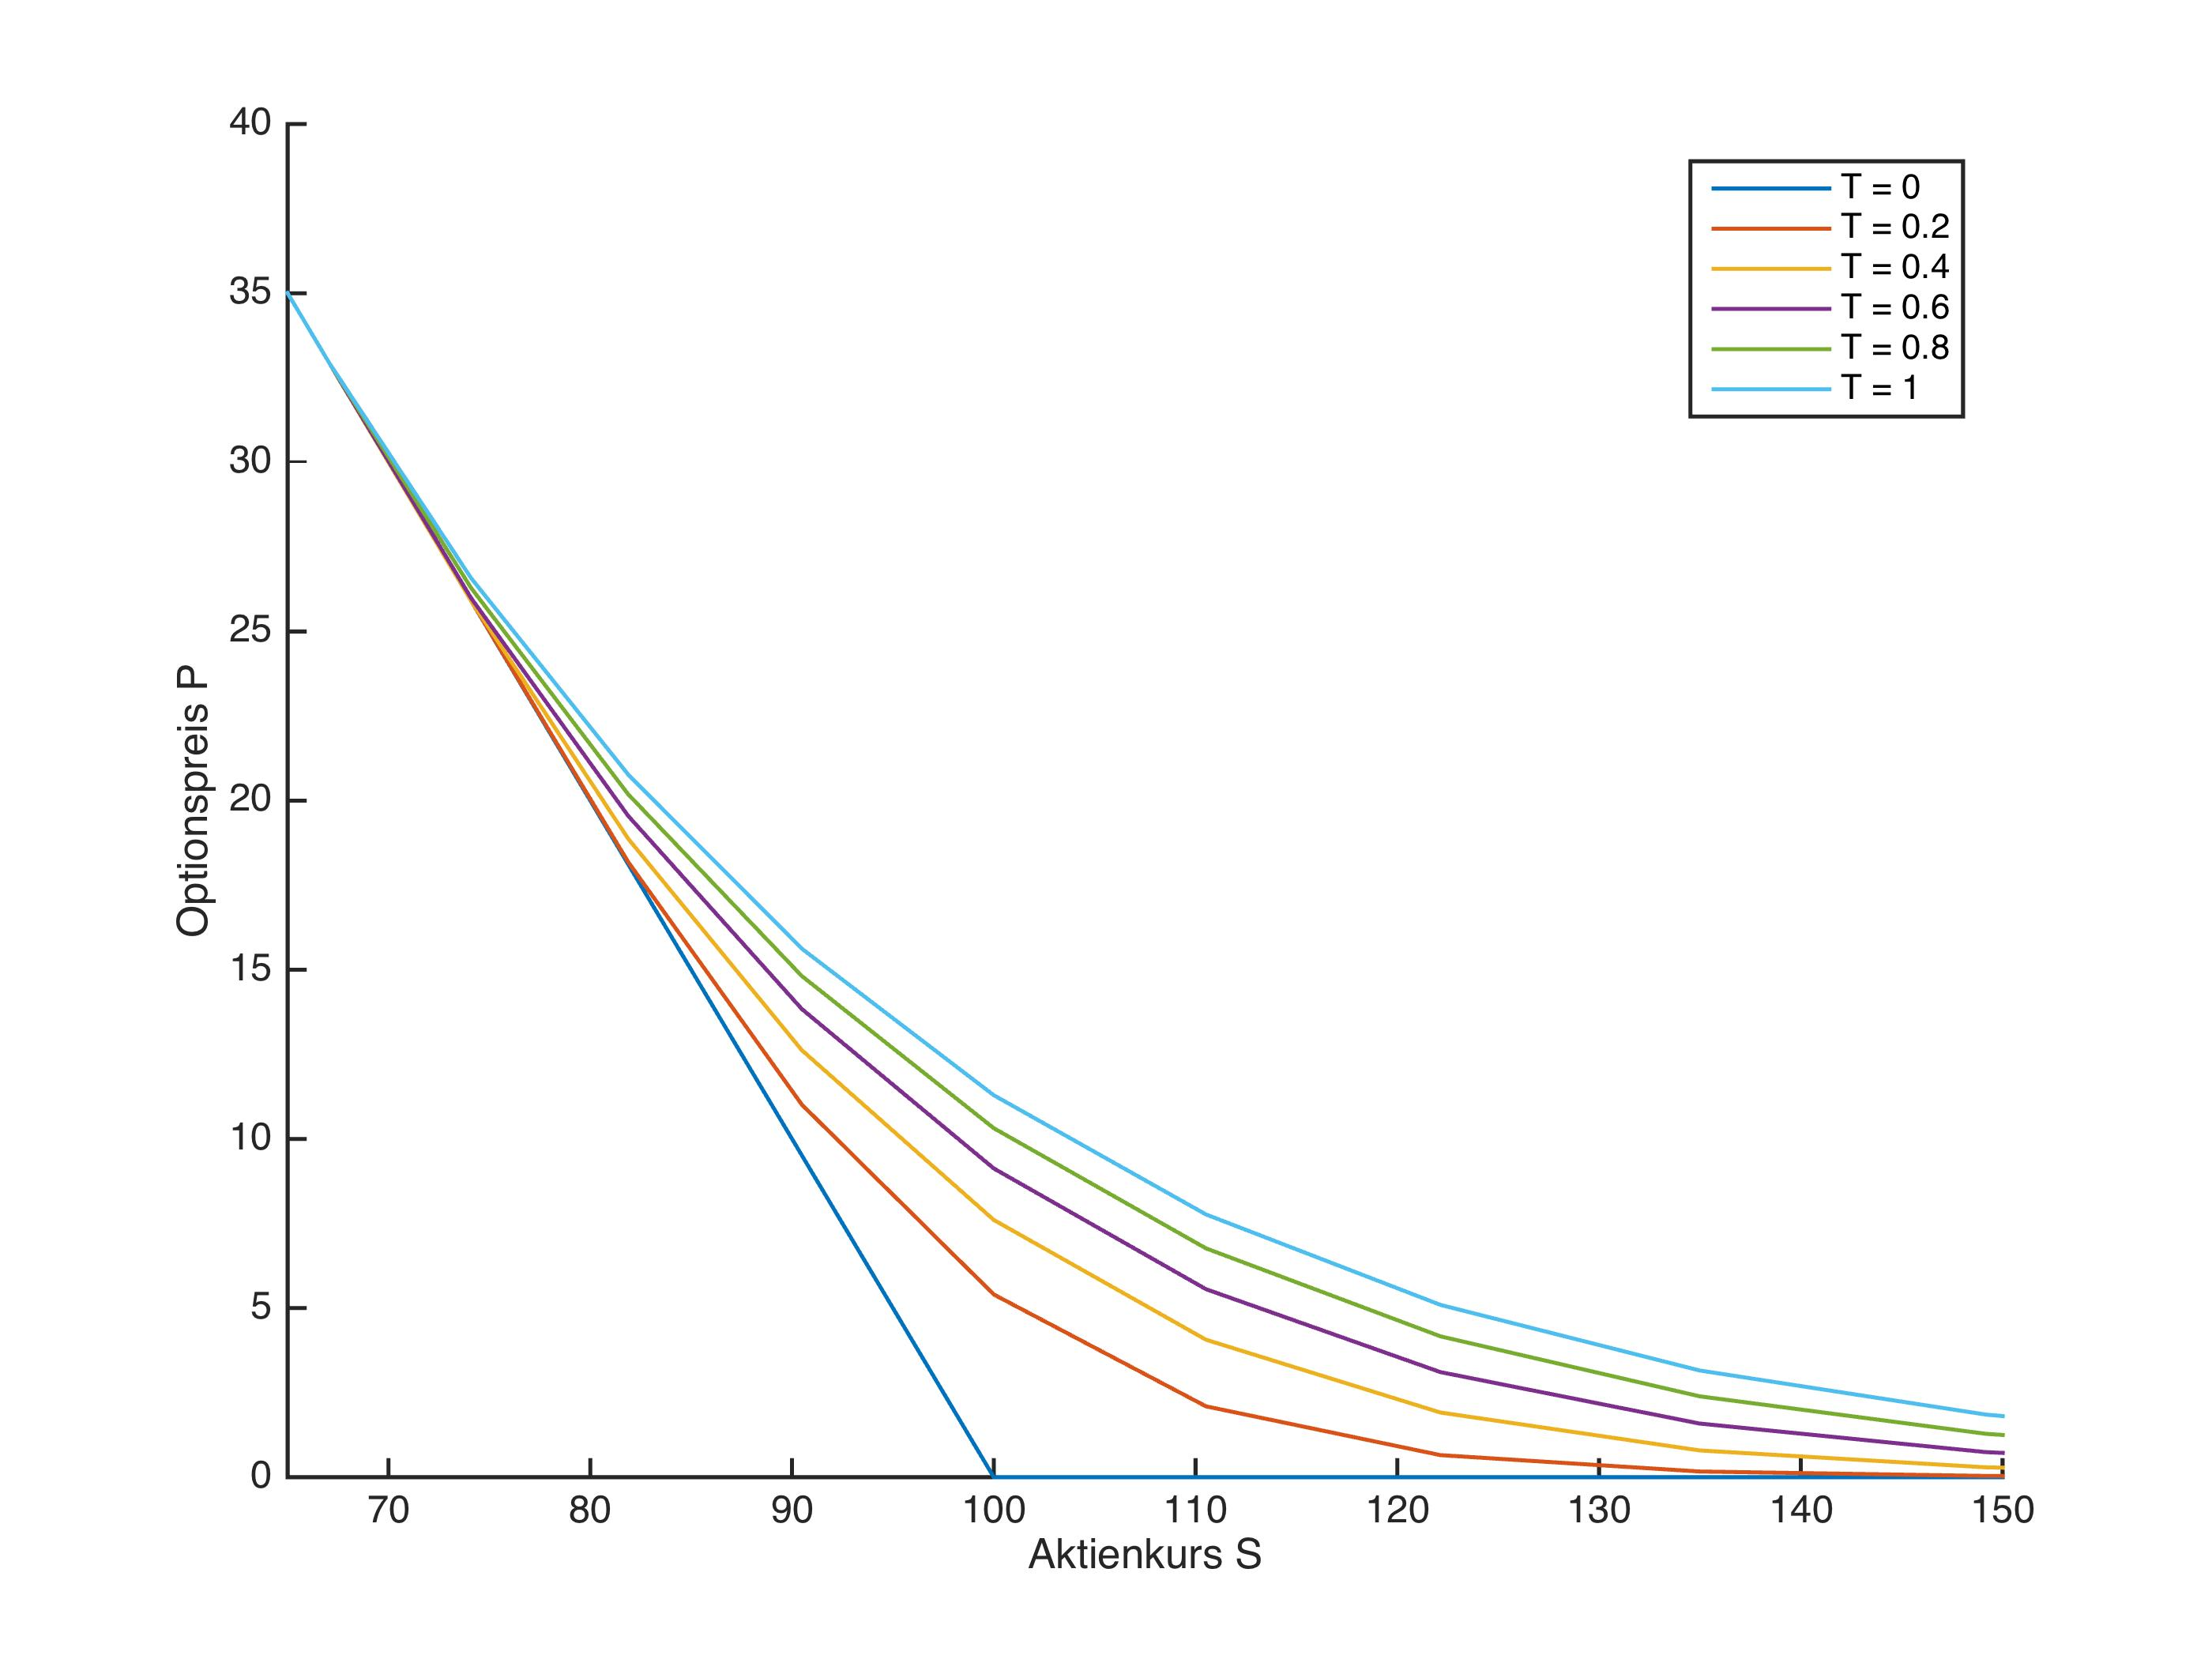
\includegraphics[width=0.9\textwidth]{AmerikanischeZeitverlauf.jpg}
%\caption{Zeitlicher Verlauf einer Amerikanischen Put-Option mit $r = 0.1$, $\sigma^2 = 0.35$, $T=1$ und $D_0 = 0.08$. Berechnet durch Diskretisierung der Wärmeleitungsgleichung mit $a=5$, $M=5$ und $N=100$.}
%\end{figure}




\appendix 

\addtocontents{toc}{\protect\setcounter{tocdepth}{1}}

\chapter{Anhang} 

%%%%%%%%%%%%%%%%%%%%%%%%%%%%%%%%%%%%%%%%%%%%%%%%%%%%%%%%%%%%%%%%%%%
\section{Verweise}                    %%%%%%%%%%%%%%%%%%%%%%%%%%%%%
%%%%%%%%%%%%%%%%%%%%%%%%%%%%%%%%%%%%%%%%%%%%%%%%%%%%%%%%%%%%%%%%%%%


%%%%% Plot der Auszahlungsfunktion der Optionen %%%%%%%%%%%%%%%%%%%%%%%%%%%%%%%%%%%
\subsection{Plot der Auszahlungsfunktionen \ref{GL:payoffCall} und \ref{GL:payoffPut} \label{Anhang:PlotPayoff}}
\begin{figure}[h]
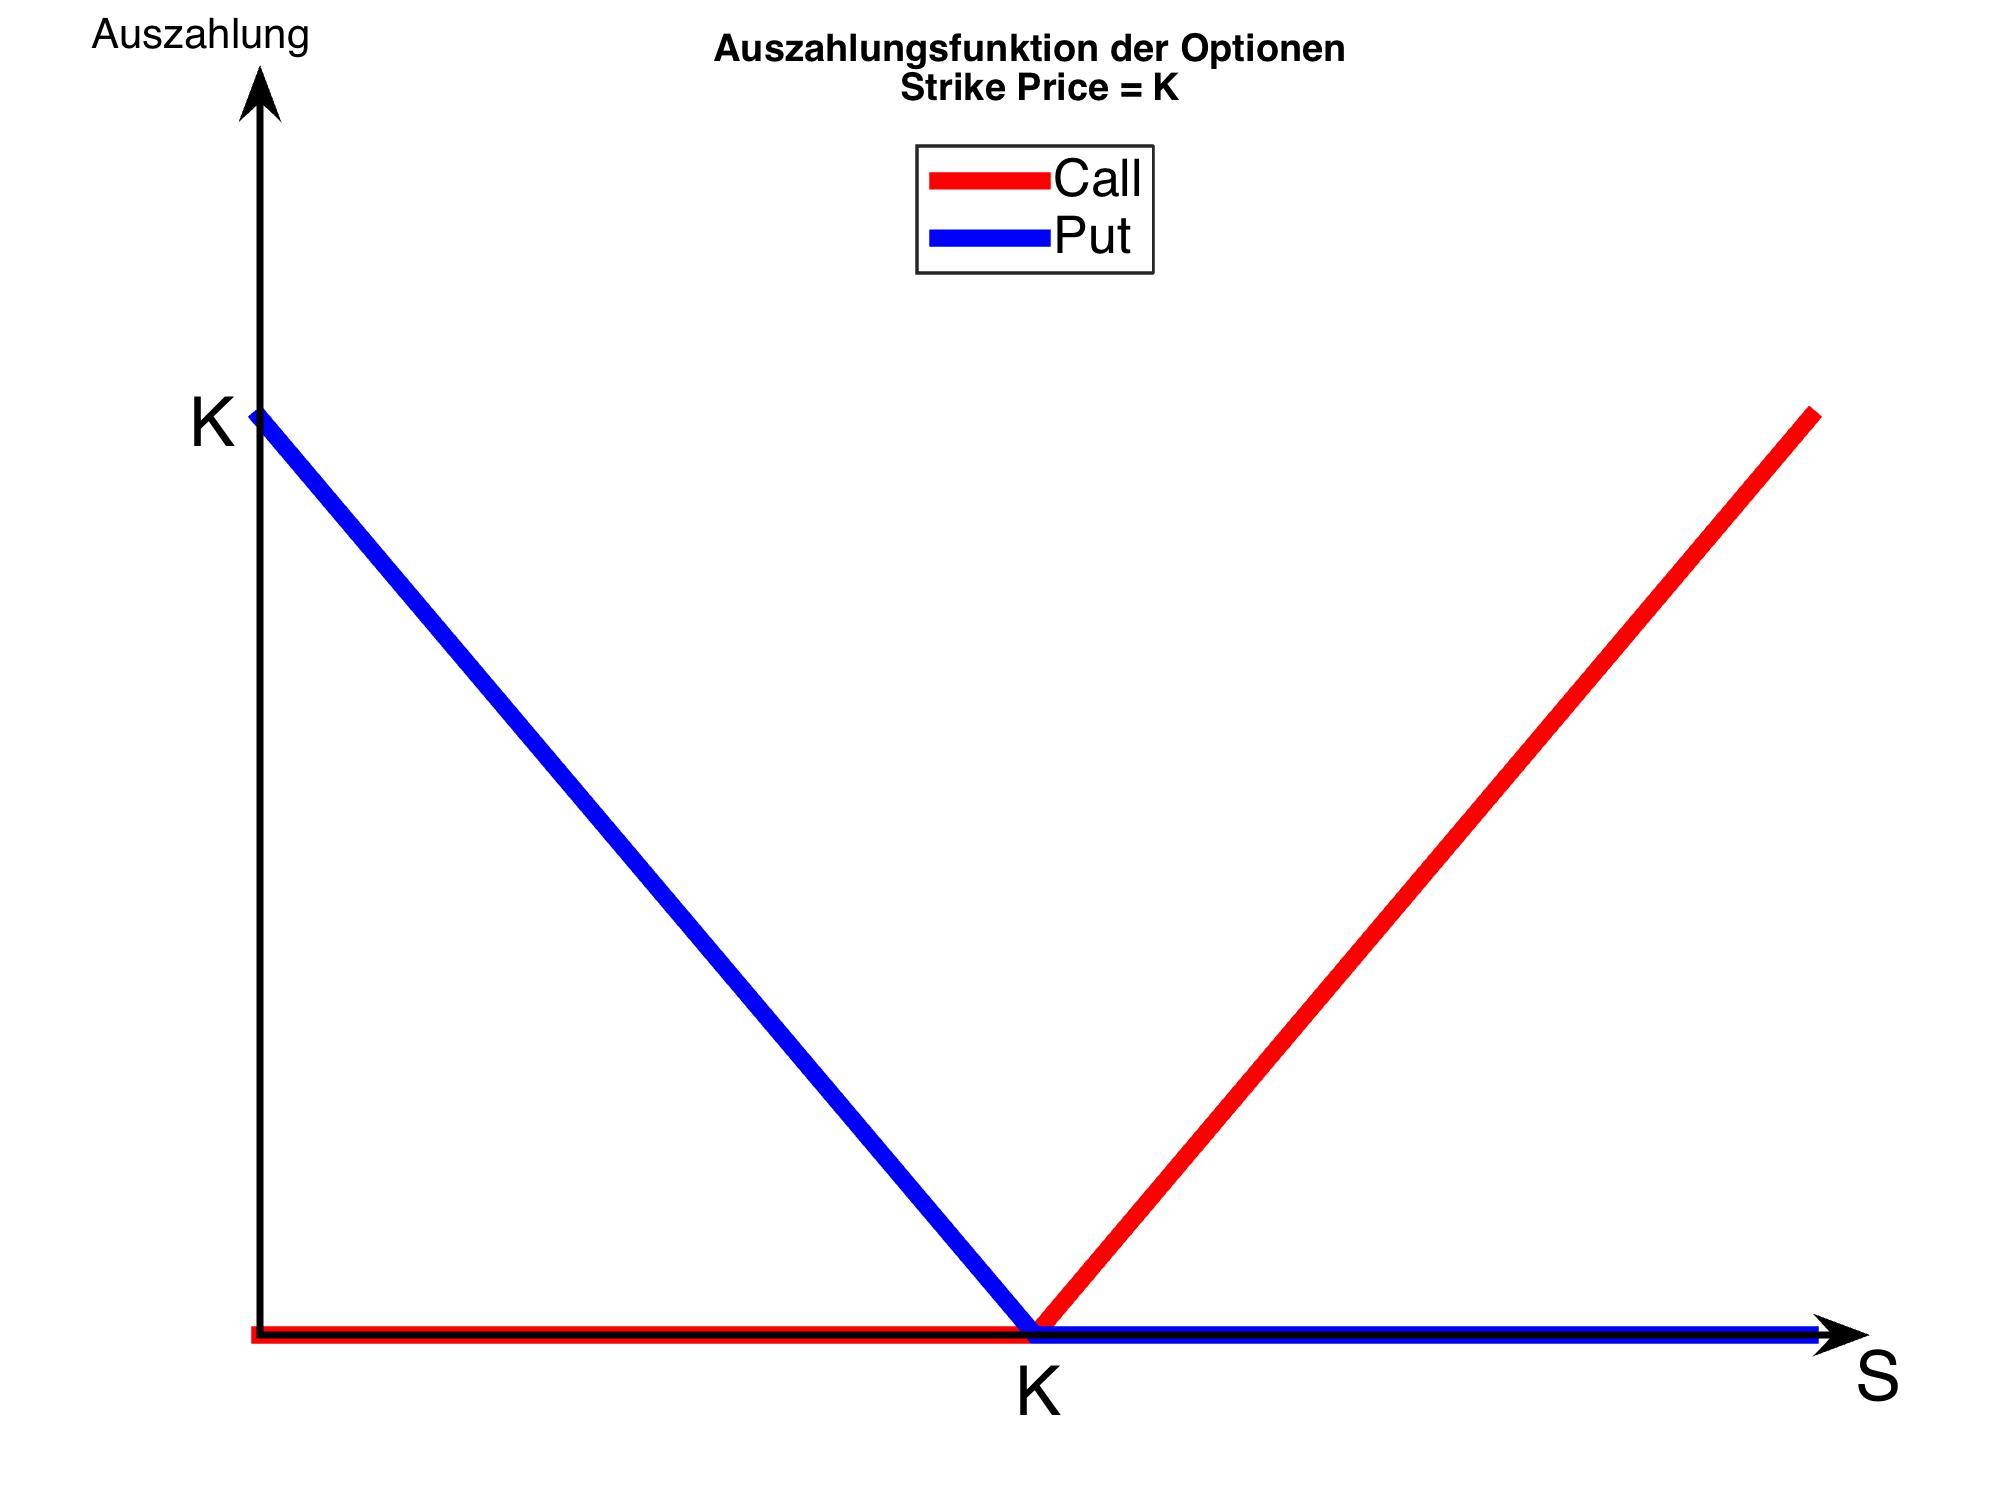
\includegraphics[width=1\textwidth]{PayoffOptionen.jpg}
\caption{Auszahlungsfunktionen einer Call- und Put-Option}
\end{figure}


%%%%% Lösung des Gleichungssystems der Duplikationsstrategie %%%%%%%%%%%%%%%%%%%%%%
\subsection{Lösung des Gleichungssystems \ref{Bin:gleichungssystem} }
\label{Anhang:LGS}
In Matrixform geschrieben ergibt sich aus (\ref{Bin:gleichungssystem}):
\begin{equation*} \begin{pmatrix}
    e^{r\Delta t} & uS \\
    e^{r\Delta t} & dS \\
\end{pmatrix} 
\begin{pmatrix}
    c_1 \\
    c_2 \\
\end{pmatrix} = 
\begin{pmatrix}
    C_u \\
    C_d \\
\end{pmatrix}
\end{equation*}
Dessen Lösung sich ergibt als
\begin{equation*}
\begin{pmatrix}
    c_1 \\
    c_2 \\
\end{pmatrix} =
\frac{1}{e^{r\Delta t}S\left(d-u\right)}
\begin{pmatrix}
    dS &  -uS \\
    -e^{r\Delta t} & e^{r\Delta t} \\
\end{pmatrix}
\begin{pmatrix}
    C_u \\
    C_d \\
\end{pmatrix} = 
\begin{pmatrix}
\frac{S\left(dC_u - uC_d\right)}{e^{r\Delta t}S\left(d-u\right)} \\
\frac{e^{r\Delta t}\left(C_d-C_u\right)}{e^{r\Delta t}S\left(d-u\right)}
\end{pmatrix}=
\begin{pmatrix}
    \frac{uC_d - dC_u}{e^{r\Delta t}(u-d)} \\
    \frac{C_u - C_d}{S(u-d)} \\
\end{pmatrix}
\end{equation*}

%%%%%%%%%%% Lösung des Gleichungssystems für die neue Wahl der Parameter %%%%%%%%%%%%%%
\subsection{Lösung des Gleichungssystems (\ref{BIN:GS1})-(\ref{BIN:GS2})}
\label{Anhang:GSParameter}

Auflösen von (\ref{BIN:GS1}) nach $p$ liefert:
\begin{equation*}
p = \frac{\left(r-\frac{1}{2}\sigma^2\right)\Delta t - ln(d)}{ln\left(\frac{u}{d}\right)}
\end{equation*}
Mit der Zusatzbedingung $d = \nicefrac{1}{u}$ und Einsetzen in (\ref{BIN:GS2}) folgt:
\begin{eqnarray*}
\sigma^2\Delta t & = & ln\left(\frac{u}{d}\right)^2\frac{\left(r-\frac{1}{2}\sigma^2\right)\Delta t - ln(d)}{ln\left(\frac{u}{d}\right)}\left(\frac{ln\left(\frac{u}{d}\right)-\left(r-\frac{1}{2}\sigma^2\right)\Delta t + ln(d)}{ln\left(\frac{u}{d}\right)}\right) \\
& = & \left(\left(r-\frac{1}{2}\sigma^2\right)\Delta t - ln(d)\right)\left(ln(u) - \left(r-\frac{1}{2}\sigma^2\right)\Delta t\right) \\
& = & -ln(u)ln(d) - \left(r-\frac{1}{2}\sigma^2\right)(\Delta t)^2 + \underbrace{(ln(u)+ln(d))}_{=0}\left(r-\frac{1}{2}\sigma^2\right)\Delta t \\
& = & ln(u)^2 + \mathcal{O}\left((\Delta t)^2\right)
\end{eqnarray*}
Unter Vernachlässigung des $\left(\Delta t\right)^2$-Termes also
\begin{equation*}
u = e^{\sigma\sqrt{\Delta t}} \text{ und } d = e^{-\sigma\sqrt{\Delta t}}
\end{equation*}
Sowie
\begin{equation*}
p = \frac{\left(r-\frac{1}{2}\sigma^2\right)\Delta t + \sigma\sqrt{\Delta t}}{2\sigma\sqrt{\Delta t}} =\frac{1}{2} + \frac{1}{2}\left(r-\frac{1}{2}\sigma^2\right)\frac{\sqrt{\Delta t}}{\sigma} 
\end{equation*}






%%%%% Taylorentwicklung für altes p %%%%%%%%%%%%%%%%%%%%%% 
\subsection{Wahl des Parameter p in (\ref{BIN:1PeriodenCall}) und (\ref{BIN:parameter})}
\label{Anhang:pundp'}
Sei $p_1 = \frac{e^{r\Delta t} - d}{u-d}$ (aus (\ref{BIN:1PeriodenCall})) und $p_2 = \frac{1}{2} + \frac{1}{2}\left(r-\frac{1}{2}\sigma^2\right)\frac{\sqrt{\Delta t}}{\sigma}$ (aus \ref{BIN:parameter})).
Da $u = e^{\sigma\sqrt{\Delta t}}$ und $d = e^{-\sigma\sqrt{\Delta t}}$, ist $p_1$ eine Funktion von $\Delta t$ und eine Taylorentwicklung liefert:
\begin{eqnarray*}
p_1 & = & \frac{\left(1+r\Delta t\right) - \left(1 - \sigma\sqrt{\Delta t} + \frac{1}{2}\sigma^2\Delta t\right) +  \mathcal{O}\left(\left(\Delta t\right)^{\nicefrac{3}{2}}\right)}{\left(1 + \sigma\sqrt{\Delta t} + \frac{1}{2}\left(\sigma\sqrt{\Delta t}\right)^2\right)- \left(1 - \sigma\sqrt{\Delta t} + \frac{1}{2}\left(\sigma\sqrt{\Delta t}\right)^2\right) + \mathcal{O}\left(\left(\Delta t\right)^{\nicefrac{3}{2}}\right)} \\
  & = & \frac{\sigma + \left(r-\frac{1}{2}\sigma^2\right)\sqrt{\Delta t} +  \mathcal{O}(\Delta t)}{2\sigma + \mathcal{O}(\Delta t)} \\
  %& = & \frac{1}{2 + \mathcal{O}(\Delta t)} + \frac{\left(r-\frac{1}{2}\sigma^2\right)}{2\sigma + \mathcal{O}(\Delta t)} \\
  %& = & \underbrace{\frac{1}{2} + \frac{1}{2}\left(r-\frac{1}{2}\sigma^2\right)\frac{\sqrt{\Delta t}}{\sigma}}_{= p'} +\,\mathcal{O}(\Delta t)
\end{eqnarray*}
Und damit
\begin{equation*}
\lim_{\Delta t \to 0} p_1 =  \lim_{\Delta t \to 0} p_2 = \frac{1}{2} \\
\end{equation*}

%%%%%%%%%%% TAYLORENTWICKLUNG FÜR p'%%%%%%%%%%%%%%%%%%%%%%%%%%%%%%%%%%%%%
\subsection{Grenzwert von $\frac{2p' - 1}{\sqrt{\Delta t}}$ in Satz \ref{BIN:konvergenzCallOption}}
\label{Anhang:Taylorp'} 
Mit $p' = pue^{-r\Delta t}$ gilt:
\begin{eqnarray*}
\frac{2p'-1}{\sqrt{\Delta t}} & = & \frac{2pue^{-r\Delta t}-1}{\sqrt{\Delta t}} \\
 & = & \frac{2\left(\frac{1}{2} + \frac{1}{2}\left(r-\frac{1}{2}\sigma^2\right)\frac{\sqrt{\Delta t}}{\sigma}\right)ue^{-r\Delta t}-1}{\sqrt{\Delta t}} \\
 & = & \left(r-\frac{1}{2}\sigma^2\right)\frac{1}{\sigma}e^{\sigma\sqrt{\Delta t}-r\Delta t} + \frac{e^{\sigma\sqrt{\Delta t}-r\Delta t} - 1}{\sqrt{\Delta t}} \\
 & \overset{\tiny Taylor}{=} & \left(r-\frac{1}{2}\sigma^2\right)\frac{1}{\sigma}\underbrace{e^{\sigma\sqrt{\Delta t}-r\Delta t}}_{\to 1} + \frac{1+\left(\sigma\sqrt{\Delta t} - r\Delta t\right) + \mathcal{O}(\Delta t) - 1}{\sqrt{\Delta t}} \\
 & \to & \frac{r}{\sigma} - \frac{\sigma}{2} + \sigma \\
 & = & \frac{r}{\sigma} + \frac{\sigma}{2} 
\end{eqnarray*}


%%%%%%%%%%%% Lösung der Differentialgleichung zum Aktienkurs St %%%%%%%%%
\subsection{Herleitung des Aktienkurses \ref{BS:aktienkurs}} \label{Anhang:HerleitungBSAktienkurs}
Mit der Differentialgleichung nach Itô \ref{BS:differentialgleichungAktie} ergeben sich der Drift $a = \mu S$ und die Diffusion $b = \sigma S$. Zudem wählen wir $f \in C^{2,1}(\mathbb{R}, \mathbb{R}^+), \; f(x,t) \mapsto ln(x)$. Wir erhalten für die Ableitungen von $f$:
\begin{equation*}
f_t = 0, \quad f_x = \frac{1}{x} \text{ und } f_{xx} = -\frac{1}{x^2} 
\end{equation*}

Damit ergibt sich mit dem Lemma von Itô \ref{GL:itosLemma}:
\begin{eqnarray*}
d\, ln(S(t)) & = & \left(\mu S \frac{1}{S} + \left(\sigma S\right)^2\left(-\frac{1}{S^2}\right)\right)dt + \sigma S\frac{1}{S} dW_s \\
& = & \left(\mu - \frac{1}{2}\sigma^2\right)dt + \sigma dW_s
\end{eqnarray*}
Was äquivalent ist zur Integralschreibweise:
\begin{eqnarray*}
ln(S(t)) & = & ln(S(0)) + \int _0^t \left(\mu - \frac{1}{2}\sigma^2\right)ds + \int _0^t \sigma dW_s \\
& = & ln(S(0)) + \left(\mu - \frac{1}{2}\sigma^2\right)t + \sigma W_t 
\end{eqnarray*}
Wobei für den speziellen Itô-Prozess $W_t$ (mit $ a = 0 $, $ b = 1$ und $f(x,t) = x$) gilt:
\begin{equation*}
W_t = \underbrace{W_0}_{=0} + \int _0^t 1 \, dW_s \Leftrightarrow \int _0^t \sigma dW_s = \sigma W_t 
\end{equation*}
und wir erhalten durch Umformung den Aktienkurs \ref{BS:aktienkurs}:
\begin{equation*}
S(t) = S(0)\,exp\left[ \left( \mu - \tfrac{1}{2}\sigma^2\right)t + \sigma W_t\right]
\end{equation*}



%%%%%%%%%% UMFORMUNGEN ZUR LÖSUNG DER WÄRMELEITUNGSGLEICHUNG %%%%%%%%%%%%%%
\subsection{Umformungen zur Lösung der Wärmeleitungsgleichung in Abschnitt \ref{cha:LoesungWaermeleitungsgleichung}} \label{Anhang:UmformungenWLG}
Ausgehend von
\begin{eqnarray*}
u(x,\tau) & = & \frac{1}{\sqrt{2\pi}}\int _{-\nicefrac{x}{\sqrt{2\tau}}}^{\infty} exp\left(\frac{1}{2}\left(k_0+1\right)\left(x+y\sqrt{2\tau}\right)\right)e^{\nicefrac{-y^2}{2}}dy \\
 &   & - \frac{1}{\sqrt{2\pi}}\int _{-\nicefrac{x}{\sqrt{2\tau}}}^{\infty} exp\left(\frac{1}{2}\left(k_0-1\right)\left(x+y\sqrt{2\tau}\right)\right)e^{\nicefrac{-y^2}{2}}dy 
\end{eqnarray*}
gilt
\begin{eqnarray*}
& & \frac{1}{\sqrt{2\pi}}\int _{-\nicefrac{x}{\sqrt{2\tau}}}^{\infty} exp\left(\frac{1}{2}\left(k_0\pm 1\right)\left(x+y\sqrt{2\tau}\right)\right)e^{\nicefrac{-y^2}{2}}dy \\
& = & \frac{exp\left(\frac{1}{2}\left(k_0\pm 1\right)x\right)}{\sqrt{2\pi}} \int _{-\nicefrac{x}{\sqrt{2\tau}}}^{\infty} exp\left(\frac{1}{2}\left(k_0+1\right)y\sqrt{2\tau}-\frac{y^2}{2}\right)dy \\
& = & \frac{exp\left(\frac{1}{2}\left(k_0\pm 1\right)x\right)}{\sqrt{2\pi}} \int _{-\nicefrac{x}{\sqrt{2\tau}}}^{\infty} exp\left(\frac{1}{4}\left(k_0 \pm 1\right)^2\tau -\frac{1}{2}\left(y-\frac{1}{2}\left(k_0\pm 1\right)\sqrt{2\tau}\right)^2\right)dy \\
& = & \frac{exp\left(\frac{1}{2}\left(k_0\pm 1\right)x + \frac{1}{4}\left(k_0 \pm 1\right)^2\tau\right)}{\sqrt{2\pi}} \int _{-\nicefrac{x}{\sqrt{2\tau}}}^{\infty} exp\left(-\frac{1}{2}\left(y-\frac{1}{2}\left(k_0\pm 1\right)\sqrt{2\tau}\right)^2\right)dy \\
& = & \frac{exp\left(\frac{1}{2}\left(k_0\pm 1\right)x + \frac{1}{4}\left(k_0 \pm 1\right)^2\tau\right)}{\sqrt{2\pi}} \int _{-\nicefrac{x}{\sqrt{2\tau}}-\frac{1}{2}\left(k_0\pm 1\right)\sqrt{2\tau}}^{\infty} exp\left(-\frac{1}{2}y^2\right)dy 
\end{eqnarray*}
Jetzt gilt für die untere Integralgrenze mit Rücktransformation in die ursprünglichen Variablen $S$, $K$, $r$, $D_0$, $\sigma$, $T$ und $t$:
\begin{eqnarray*}
-\frac{x}{\sqrt{2\tau}}-\frac{1}{2}\left(k_0\pm 1\right)\sqrt{2\tau} & = & \frac{-ln\left(\nicefrac{S}{K}\right)}{\sqrt{\sigma^2(T-t)}} - \frac{1}{2}\left(\frac{2\left(r-D_0\right)}{\sigma^2} \pm 1\right)\sqrt{2\sigma^2(T-t)} \\
& = & \frac{-ln\left(\nicefrac{S}{K}\right) -\frac{1}{2}\left(\frac{2\left(r-D_0\right)\pm\sigma^2}{\sigma^2}\right)\sigma^2(T-t)}{\sqrt{\sigma^2(T-t)}} \\
& = & \frac{-ln\left(\nicefrac{S}{K}\right) -\left(\left(r-D_0\right)\pm\frac{1}{2}\sigma^2\right)\left(T-t\right)}{\sigma\sqrt{(T-t)}} \\
& = & - d_{\nicefrac{1}{2}}
\end{eqnarray*}
und damit 
\begin{eqnarray*}
& & exp\left(\frac{1}{2}\left(k_0\pm 1\right)x + \frac{1}{4}\left(k_0 \pm 1\right)^2\tau\right)\frac{1}{\sqrt{2\pi}} \int _{-\nicefrac{x}{\sqrt{2\tau}}-\frac{1}{2}\left(k_0\pm 1\right)\sqrt{2\tau}}^{\infty} exp\left(-\frac{1}{2}y^2\right)dy \\
& = & exp\left(\tfrac{1}{2}\left(k_0 \pm 1\right)x + \tfrac{1}{4}\left(k_0 \pm 1\right)^2\tau\right)\left(1-\Phi\left(-d_{\nicefrac{1}{2}}\right)\right)\\
& = & exp\left(\tfrac{1}{2}\left(k_0 \pm 1\right)x + \tfrac{1}{4}\left(k_0 \pm 1\right)^2\tau\right)\Phi\left(d_{\nicefrac{1}{2}}\right)
\end{eqnarray*} 



%%%%%%%%%%
\newpage%%
%%%%%%%%%%%%%%%%%%%%%%%%%%%%%%%%%%%%%%%%%%%%%%%%%%%%%%%%%%%%%%%%%%%%%%%%%%
\section{MATLAB Programme}                 %%%%%%%%%%%%%%%%%%%%%%%%%%%%%%%
%%%%%%%%%%%%%%%%%%%%%%%%%%%%%%%%%%%%%%%%%%%%%%%%%%%%%%%%%%%%%%%%%%%%%%%%%%

%%%%%%%%%%%%%%%%%%%%%%%%%%%%%%%%%%%%%%%%%%%%
\subsection{Programme zu Kapitel 3} %%%%%%%%BinbaumEuro
\label{Anhang:ProgrammeKapitel3}    %%%%%%%%
%%%%%%%%%%%%%%%%%%%%%%%%%%%%%%%%%%%%%%%%%%%%
\lstinputlisting[breaklines=true,caption = {MATLAB Funktion zur Berechnung europäischer Optionen},label = BinbaumEuro,captionpos=b]{Matlab/BinbaumEuro.m}

\lstinputlisting[breaklines=true,caption = {MATLAB Funktion zur Berechnung einer Amerikanischen Put-Option},label = BinbaumAPut,captionpos=b]{Matlab/BinbaumAPut.m}



%%%%%%%%%%%%%%%%%%%%%%%%%%%%%%%%%%%%%%%%%%%%
\subsection{Programm zu Kapitel 4}  %%%%%%%%AmericanPut
\label{Anhang:ProgrammKapitel4}     %%%%%%%%
%%%%%%%%%%%%%%%%%%%%%%%%%%%%%%%%%%%%%%%%%%%%
\lstinputlisting[breaklines=true,label=AmericanPut,captionpos=b,caption={MATLAB Funktion zur Bewertung einer Amerikanischen Put-Option.}]{Matlab/AmericanPut.m}
Falls wir in der Funktion \ref{AmericanPut} das $f$ der Nebenbedingung (Zeile 14) zu 
\begin{lstlisting}[numbers=none]
f(:,j) = exp(0.5*(k0-1)*x + (0.25*(k0-1)^2+k)*(j-1)*s*ones(1,N+1))'.*max(0,exp(x)-1)';
\end{lstlisting}
sowie die Reihenfolge der Gleichungssysteme zu $Gv=b$ gefolgt von $G^Tu=v$ ändern, bewerten wir eine Amerikanische Call-Option.

Und wenn man jeweils die Kontrolle der Nebenbedingung in Zeile 49 weglässt, bewertet man die entsprechende Europäische Option.




% Einbinden aller Bücher 
\nocite{*}
\bibliography{bibliographie}

% Eidesstattliche Erklärung
\addchap{Eidesstattliche Erklärung}
Ich, \autor, Matrikel-Nr.\ \matrikelnr, versichere hiermit, dass ich meine Bachelorarbeit mit dem Thema
\begin{quote}
\textit{\titel} \textit{\untertitel}
\end{quote}
selbständig verfasst und keine anderen als die angegebenen Quellen und Hilfsmittel benutzt habe, wobei ich alle wörtlichen und sinngemäßen Zitate als solche gekennzeichnet habe. Die Arbeit wurde bisher keiner anderen Prüfungsbehörde vorgelegt und auch nicht veröffentlicht.

\vspace{1.2cm}
\ort, den \today

\vspace{1cm}
\rule[-0.2cm]{8cm}{0.5pt}

\textsc{\autor} 

\end{document}







